% Thanks to Project GutenMark
% Source: http://www.sandroid.org/GutenMark/wasftp.GutenMark/MarkedTexts/

%% LyX 1.3 created this file.  For more info, see http://www.lyx.org/.
%% Do not edit unless you really know what you are doing.
\documentclass[12pt,english]{book}
\usepackage{newcent}
\usepackage[T1]{fontenc}
\usepackage[latin1]{inputenc}
\usepackage{geometry}
\geometry{verbose,paperwidth=5.5in,paperheight=8.5in,tmargin=1in,bmargin=1in,lmargin=1in,rmargin=1in}
\setcounter{secnumdepth}{3}
\setcounter{tocdepth}{3}
\usepackage{graphicx}

\makeatletter

%%%%%%%%%%%%%%%%%%%%%%%%%%%%%% LyX specific LaTeX commands.
\newcommand{\noun}[1]{\textsc{#1}}

\usepackage{babel}
\makeatother
\begin{document}
\sloppy

\evensidemargin = -0.25in

\oddsidemargin = 0.25in

\hyphenation{Sher-lock}

\pagestyle{empty}

\newcommand{\mdsh}[1]{\mbox{#1}\linebreak[1]}

\date{}

\raggedbottom


\title{A Study in Scarlet}


\author{Sir Arthur Conan Doyle\\
{\normalsize Illustrations by Richard Gutschmidt}}

\maketitle
\vspace*{\stretch{1}}

\noindent This public-domain (U.S.) text was prepared directly from
an 1887 edition, and care has been taken to duplicate the original
exactly, including typographical and punctuation vagaries. Thanks
to Randolph Cox for providing the book for etexting. Etext prepared
by Roger Squires <rsquires@unm.edu>.

\bigskip{}
\noindent The resulting Project Gutenberg edition ({}``study10'')
was converted to \LaTeX{} using \textbf{GutenMark} software and re-edited
(mainly formatting) by Ron Burkey. A footnote lacking in the Project
Gutenberg edition was also restored. Report problems to <info@birdsproject.org>.
Since the intent of this edition was easy readability, extensive notes
concerning preparaton of the etext that appeared in the Project Gutenberg
edition (described above) were removed. Refer to the Project Gutenberg
edition if you are interested in these details.

\begin{description}
\item [B~12/13/02]Proofing completed.
\item [C~12/31/02]Added illustrations, from the 1902 Robert Lutz Verlag
(German) edition, as archived at bakerstreet221b.de.
\item [D~06/13/03]\LaTeX{} mdashes corrected.
\end{description}
\vspace{\stretch{1}}

\frontmatter

\pagestyle{myheadings} {\footnotesize \tableofcontents{}}\newpage


\mainmatter



\part*{PART I.\protect \\
{\normalsize (}\textit{\normalsize Being a reprint from the reminiscences
of} \noun{\normalsize John H.\ Watson, M.D.}{\normalsize ,} \textit{\normalsize late
of the Army Medical Department.}{\normalsize )}}

\addcontentsline{toc}{part}{PART I}

\markboth{A STUDY IN SCARLET}{PART I}


\chapter*{\raggedright CHAPTER I. MR.\ SHERLOCK HOLMES.}



\addcontentsline{toc}{chapter}{CHAPTER I. MR.\ SHERLOCK HOLMES.}

\markboth{A STUDY IN SCARLET}{CHAPTER I}

In the year 1878 I took my degree of Doctor of Medicine of the University
of London, and proceeded to Netley to go through the course prescribed
for surgeons in the army. Having completed my studies there, I was
duly attached to the Fifth Northumberland Fusiliers as Assistant Surgeon.
The regiment was stationed in India at the time, and before I could
join it, the second Afghan war had broken out. On landing at Bombay,
I learned that my corps had advanced through the passes, and was already
deep in the enemy's country. I followed, however, with many other
officers who were in the same situation as myself, and succeeded in
reaching Candahar in safety, where I found my regiment, and at once
entered upon my new duties.

The campaign brought honours and promotion to many, but for me it
had nothing but misfortune and disaster. I was removed from my brigade
and attached to the Berkshires, with whom I served at the fatal battle
of Maiwand. There I was struck on the shoulder by a Jezail bullet,
which shattered the bone and grazed the subclavian artery. %
\begin{figure}[htbp]
\noindent \begin{center}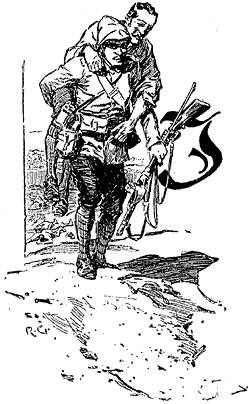
\includegraphics{images/study10-stud-01.png}\end{center}

\noindent \begin{center}\noun{I should have fallen into the hands
of the murderous Ghazis had it not been for the devotion and courage
shown by Murray, my orderly.}\end{center}
\end{figure}
I should have fallen into the hands of the murderous Ghazis had it
not been for the devotion and courage shown by Murray, my orderly,
who threw me across a pack-horse, and succeeded in bringing me safely
to the British lines.

Worn with pain, and weak from the prolonged hardships which I had
undergone, I was removed, with a great train of wounded sufferers,
to the base hospital at Peshawar. Here I rallied, and had already
improved so far as to be able to walk about the wards, and even to
bask a little upon the verandah, when I was struck down by enteric
fever, that curse of our Indian possessions. For months my life was
despaired of, and when at last I came to myself and became convalescent,
I was so weak and emaciated that a medical board determined that not
a day should be lost in sending me back to England. I was dispatched,
accordingly, in the troopship {}``Orontes,'' and landed a month
later on Portsmouth jetty, with my health irretrievably ruined, but
with permission from a paternal government to spend the next nine
months in attempting to improve it.

I had neither kith nor kin in England, and was therefore as free as
air\mdsh{---}or as free as an income of eleven shillings and sixpence
a day will permit a man to be. Under such circumstances, I naturally
gravitated to London, that great cesspool into which all the loungers
and idlers of the Empire are irresistibly drained. There I stayed
for some time at a private hotel in the Strand, leading a comfortless,
meaningless existence, and spending such money as I had, considerably
more freely than I ought. So alarming did the state of my finances
become, that I soon realized that I must either leave the metropolis
and rusticate somewhere in the country, or that I must make a complete
alteration in my style of living. Choosing the latter alternative,
I began by making up my mind to leave the hotel, and to take up my
quarters in some less pretentious and less expensive domicile.

On the very day that I had come to this conclusion, I was standing
at the Criterion Bar, when some one tapped me on the shoulder, and
turning round I recognized young Stamford, who had been a dresser
under me at Barts. The sight of a friendly face in the great wilderness
of London is a pleasant thing indeed to a lonely man. In old days
Stamford had never been a particular crony of mine, but now I hailed
him with enthusiasm, and he, in his turn, appeared to be delighted
to see me. In the exuberance of my joy, I asked him to lunch with
me at the Holborn, and we started off together in a hansom.

{}``Whatever have you been doing with yourself, Watson?'' he asked
in undisguised wonder, as we rattled through the crowded London streets.
{}``You are as thin as a lath and as brown as a nut.''

I gave him a short sketch of my adventures, and had hardly concluded
it by the time that we reached our destination.

{}``Poor devil!'' he said, commiseratingly, after he had listened
to my misfortunes. {}``What are you up to now?''

{}``Looking for lodgings.'' I answered. {}``Trying to solve the
problem as to whether it is possible to get comfortable rooms at a
reasonable price.''

{}``That's a strange thing,'' remarked my companion; {}``you are
the second man to-day that has used that expression to me.''

{}``And who was the first?'' I asked.

{}``A fellow who is working at the chemical laboratory up at the
hospital. He was bemoaning himself this morning because he could not
get someone to go halves with him in some nice rooms which he had
found, and which were too much for his purse.''

{}``By Jove!'' I cried, {}``if he really wants someone to share
the rooms and the expense, I am the very man for him. I should prefer
having a partner to being alone.''

Young Stamford looked rather strangely at me over his wine-glass.
{}``You don't know Sherlock Holmes yet,'' he said; {}``perhaps
you would not care for him as a constant companion.''

{}``Why, what is there against him?''

{}``Oh, I didn't say there was anything against him. He is a little
queer in his ideas\mdsh{---}an enthusiast in some branches of science.
As far as I know he is a decent fellow enough.''

{}``A medical student, I suppose?'' said I.

{}``No\mdsh{---}I have no idea what he intends to go in for. I believe
he is well up in anatomy, and he is a first-class chemist; but, as
far as I know, he has never taken out any systematic medical classes.
His studies are very desultory and eccentric, but he has amassed a
lot of out-of-the way knowledge which would astonish his professors.''

{}``Did you never ask him what he was going in for?'' I asked.

{}``No; he is not a man that it is easy to draw out, though he can
be communicative enough when the fancy seizes him.''

{}``I should like to meet him,'' I said. {}``If I am to lodge with
anyone, I should prefer a man of studious and quiet habits. I am not
strong enough yet to stand much noise or excitement. I had enough
of both in Afghanistan to last me for the remainder of my natural
existence. How could I meet this friend of yours?''

{}``He is sure to be at the laboratory,'' returned my companion.
{}``He either avoids the place for weeks, or else he works there
from morning to night. If you like, we shall drive round together
after luncheon.''

{}``Certainly,'' I answered, and the conversation drifted away into
other channels.

As we made our way to the hospital after leaving the Holborn, Stamford
gave me a few more particulars about the gentleman whom I proposed
to take as a fellow-lodger.

{}``You mustn't blame me if you don't get on with him,'' he said;
{}``I know nothing more of him than I have learned from meeting him
occasionally in the laboratory. You proposed this arrangement, so
you must not hold me responsible.''

{}``If we don't get on it will be easy to part company,'' I answered.
{}``It seems to me, Stamford,'' I added, looking hard at my companion,
{}``that you have some reason for washing your hands of the matter.
Is this fellow's temper so formidable, or what is it? Don't be mealy-mouthed
about it.''

{}``It is not easy to express the inexpressible,'' he answered with
a laugh. {}``Holmes is a little too scientific for my tastes\mdsh{---}it
approaches to cold-bloodedness. I could imagine his giving a friend
a little pinch of the latest vegetable alkaloid, not out of malevolence,
you understand, but simply out of a spirit of inquiry in order to
have an accurate idea of the effects. To do him justice, I think that
he would take it himself with the same readiness. He appears to have
a passion for definite and exact knowledge.''

{}``Very right too.''

{}``Yes, but it may be pushed to excess. When it comes to beating
the subjects in the dissecting-rooms with a stick, it is certainly
taking rather a bizarre shape.''

{}``Beating the subjects!''

{}``Yes, to verify how far bruises may be produced after death. I
saw him at it with my own eyes.''

{}``And yet you say he is not a medical student?''

{}``No. Heaven knows what the objects of his studies are. But here
we are, and you must form your own impressions about him.'' As he
spoke, we turned down a narrow lane and passed through a small side-door,
which opened into a wing of the great hospital. It was familiar ground
to me, and I needed no guiding as we ascended the bleak stone staircase
and made our way down the long corridor with its vista of whitewashed
wall and dun-coloured doors. Near the further end a low arched passage
branched away from it and led to the chemical laboratory.

This was a lofty chamber, lined and littered with countless bottles.
Broad, low tables were scattered about, which bristled with retorts,
test-tubes, and little Bunsen lamps, with their blue flickering flames.
There was only one student in the room, who was bending over a distant
table absorbed in his work. At the sound of our steps he glanced round
and sprang to his feet with a cry of pleasure. %
\begin{figure}[htbp]
\noindent \begin{center}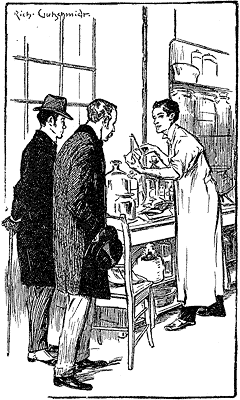
\includegraphics{images/study10-stud-02.png}\end{center}

\noindent \begin{center}\noun{{}``I've found it! I've found it,''
he shouted to my companion.}\end{center}
\end{figure}
{}``I've found it! I've found it,'' he shouted to my companion,
running towards us with a test-tube in his hand. {}``I have found
a re-agent which is precipitated by h\ae moglobin, and by nothing
else.'' Had he discovered a gold mine, greater delight could not
have shone upon his features.

{}``Dr.\ Watson, Mr.\ Sherlock Holmes,'' said Stamford, introducing
us.

{}``How are you?'' he said cordially, gripping my hand with a strength
for which I should hardly have given him credit. {}``You have been
in Afghanistan, I perceive.''

{}``How on earth did you know that?'' I asked in astonishment.

{}``Never mind,'' said he, chuckling to himself. {}``The question
now is about h\ae moglobin. No doubt you see the significance of
this discovery of mine?''

{}``It is interesting, chemically, no doubt,'' I answered, {}``but
practically\mdsh{---}''

{}``Why, man, it is the most practical medico-legal discovery for
years. Don't you see that it gives us an infallible test for blood
stains. Come over here now!'' He seized me by the coat-sleeve in
his eagerness, and drew me over to the table at which he had been
working. {}``Let us have some fresh blood,'' he said, digging a
long bodkin into his finger, and drawing off the resulting drop of
blood in a chemical pipette. {}``Now, I add this small quantity of
blood to a litre of water. You perceive that the resulting mixture
has the appearance of pure water. The proportion of blood cannot be
more than one in a million. I have no doubt, however, that we shall
be able to obtain the characteristic reaction.'' As he spoke, he
threw into the vessel a few white crystals, and then added some drops
of a transparent fluid. In an instant the contents assumed a dull
mahogany colour, and a brownish dust was precipitated to the bottom
of the glass jar.

{}``Ha! ha!'' he cried, clapping his hands, and looking as delighted
as a child with a new toy. {}``What do you think of that?''

{}``It seems to be a very delicate test,'' I remarked.

{}``Beautiful! beautiful! The old Guiacum test was very clumsy and
uncertain. So is the microscopic examination for blood corpuscles.
The latter is valueless if the stains are a few hours old. Now, this
appears to act as well whether the blood is old or new. Had this test
been invented, there are hundreds of men now walking the earth who
would long ago have paid the penalty of their crimes.''

{}``Indeed!'' I murmured.

{}``Criminal cases are continually hinging upon that one point. A
man is suspected of a crime months perhaps after it has been committed.
His linen or clothes are examined, and brownish stains discovered
upon them. Are they blood stains, or mud stains, or rust stains, or
fruit stains, or what are they? That is a question which has puzzled
many an expert, and why? Because there was no reliable test. Now we
have the Sherlock Holmes' test, and there will no longer be any difficulty.''

His eyes fairly glittered as he spoke, and he put his hand over his
heart and bowed as if to some applauding crowd conjured up by his
imagination.

{}``You are to be congratulated,'' I remarked, considerably surprised
at his enthusiasm.

{}``There was the case of Von Bischoff at Frankfort last year. He
would certainly have been hung had this test been in existence. Then
there was Mason of Bradford, and the notorious Muller, and Lefevre
of Montpellier, and Samson of new Orleans. I could name a score of
cases in which it would have been decisive.''

{}``You seem to be a walking calendar of crime,'' said Stamford
with a laugh. {}``You might start a paper on those lines. Call it
the `Police News of the Past.'''

{}``Very interesting reading it might be made, too,'' remarked Sherlock
Holmes, sticking a small piece of plaster over the prick on his finger.
{}``I have to be careful,'' he continued, turning to me with a smile,
{}``for I dabble with poisons a good deal.'' He held out his hand
as he spoke, and I noticed that it was all mottled over with similar
pieces of plaster, and discoloured with strong acids.

{}``We came here on business,'' said Stamford, sitting down on a
high three-legged stool, and pushing another one in my direction with
his foot. {}``My friend here wants to take diggings, and as you were
complaining that you could get no one to go halves with you, I thought
that I had better bring you together.''

Sherlock Holmes seemed delighted at the idea of sharing his rooms
with me. {}``I have my eye on a suite in Baker Street,'' he said,
{}``which would suit us down to the ground. You don't mind the smell
of strong tobacco, I hope?''

{}``I always smoke `ship's' myself,'' I answered.

{}``That's good enough. I generally have chemicals about, and occasionally
do experiments. Would that annoy you?''

{}``By no means.''

{}``Let me see\mdsh{---}what are my other shortcomings. I get in
the dumps at times, and don't open my mouth for days on end. You must
not think I am sulky when I do that. Just let me alone, and I'll soon
be right. What have you to confess now? It's just as well for two
fellows to know the worst of one another before they begin to live
together.''

I laughed at this cross-examination. {}``I keep a bull pup,'' I
said, {}``and I object to rows because my nerves are shaken, and
I get up at all sorts of ungodly hours, and I am extremely lazy. I
have another set of vices when I'm well, but those are the principal
ones at present.''

{}``Do you include violin-playing in your category of rows?'' he
asked, anxiously.

{}``It depends on the player,'' I answered. {}``A well-played violin
is a treat for the gods\mdsh{---}a badly-played one\mdsh{---}''

{}``Oh, that's all right,'' he cried, with a merry laugh. {}``I
think we may consider the thing as settled\mdsh{---}that is, if the
rooms are agreeable to you.''

{}``When shall we see them?''

{}``Call for me here at noon to-morrow, and we'll go together and
settle everything,'' he answered.

{}``All right\mdsh{---}noon exactly,'' said I, shaking his hand.

We left him working among his chemicals, and we walked together towards
my hotel.

{}``By the way,'' I asked suddenly, stopping and turning upon Stamford,
{}``how the deuce did he know that I had come from Afghanistan?''

My companion smiled an enigmatical smile. {}``That's just his little
peculiarity,'' he said. {}``A good many people have wanted to know
how he finds things out.''

{}``Oh!\ a mystery is it?''\ I cried, rubbing my hands. {}``This
is very piquant. I am much obliged to you for bringing us together.\ 
`The proper study of mankind is man,' you know.''

{}``You must study him, then,'' Stamford said, as he bade me good-bye.
{}``You'll find him a knotty problem, though. I'll wager he learns
more about you than you about him. Good-bye.''

{}``Good-bye,'' I answered, and strolled on to my hotel, considerably
interested in my new acquaintance.


\chapter*{\raggedright CHAPTER II. THE SCIENCE OF DEDUCTION.}

\addcontentsline{toc}{chapter}{CHAPTER II. THE SCIENCE OF\\
DEDUCTION. }

\markboth{A STUDY IN SCARLET}{CHAPTER II}

We met next day as he had arranged, and inspected the rooms at No.\ \noun{221b},
Baker Street, of which he had spoken at our meeting. They consisted
of a couple of comfortable bed-rooms and a single large airy sitting-room,
cheerfully furnished, and illuminated by two broad windows. So desirable
in every way were the apartments, and so moderate did the terms seem
when divided between us, that the bargain was concluded upon the spot,
and we at once entered into possession. That very evening I moved
my things round from the hotel, and on the following morning Sherlock
Holmes followed me with several boxes and portmanteaus. For a day
or two we were busily employed in unpacking and laying out our property
to the best advantage. That done, we gradually began to settle down
and to accommodate ourselves to our new surroundings.

Holmes was certainly not a difficult man to live with. He was quiet
in his ways, and his habits were regular. It was rare for him to be
up after ten at night, and he had invariably breakfasted and gone
out before I rose in the morning. Sometimes he spent his day at the
chemical laboratory, sometimes in the dissecting-rooms, and occasionally
in long walks, which appeared to take him into the lowest portions
of the City. Nothing could exceed his energy when the working fit
was upon him; but now and again a reaction would seize him, and for
days on end he would lie upon the sofa in the sitting-room, hardly
uttering a word or moving a muscle from morning to night. On these
occasions I have noticed such a dreamy, vacant expression in his eyes,
that I might have suspected him of being addicted to the use of some
narcotic, had not the temperance and cleanliness of his whole life
forbidden such a notion.

As the weeks went by, my interest in him and my curiosity as to his
aims in life, gradually deepened and increased. His very person and
appearance were such as to strike the attention of the most casual
observer. In height he was rather over six feet, and so excessively
lean that he seemed to be considerably taller. His eyes were sharp
and piercing, save during those intervals of torpor to which I have
alluded; and his thin, hawk-like nose gave his whole expression an
air of alertness and decision. His chin, too, had the prominence and
squareness which mark the man of determination. His hands were invariably
blotted with ink and stained with chemicals, yet he was possessed
of extraordinary delicacy of touch, as I frequently had occasion to
observe when I watched him manipulating his fragile philosophical
instruments.

The reader may set me down as a hopeless busybody, when I confess
how much this man stimulated my curiosity, and how often I endeavoured
to break through the reticence which he showed on all that concerned
himself. Before pronouncing judgment, however, be it remembered, how
objectless was my life, and how little there was to engage my attention.
My health forbade me from venturing out unless the weather was exceptionally
genial, and I had no friends who would call upon me and break the
monotony of my daily existence. Under these circumstances, I eagerly
hailed the little mystery which hung around my companion, and spent
much of my time in endeavouring to unravel it.

He was not studying medicine. He had himself, in reply to a question,
confirmed Stamford's opinion upon that point. Neither did he appear
to have pursued any course of reading which might fit him for a degree
in science or any other recognized portal which would give him an
entrance into the learned world. Yet his zeal for certain studies
was remarkable, and within eccentric limits his knowledge was so extraordinarily
ample and minute that his observations have fairly astounded me. Surely
no man would work so hard or attain such precise information unless
he had some definite end in view. Desultory readers are seldom remarkable
for the exactness of their learning. No man burdens his mind with
small matters unless he has some very good reason for doing so.

His ignorance was as remarkable as his knowledge. Of contemporary
literature, philosophy and politics he appeared to know next to nothing.
Upon my quoting Thomas Carlyle, he inquired in the naivest way who
he might be and what he had done. My surprise reached a climax, however,
when I found incidentally that he was ignorant of the Copernican Theory
and of the composition of the Solar System. That any civilized human
being in this nineteenth century should not be aware that the earth
travelled round the sun appeared to be to me such an extraordinary
fact that I could hardly realize it.

{}``You appear to be astonished,'' he said, smiling at my expression
of surprise. {}``Now that I do know it I shall do my best to forget
it.''

{}``To forget it!''

{}``You see,'' he explained, {}``I consider that a man's brain
originally is like a little empty attic, and you have to stock it
with such furniture as you choose. A fool takes in all the lumber
of every sort that he comes across, so that the knowledge which might
be useful to him gets crowded out, or at best is jumbled up with a
lot of other things so that he has a difficulty in laying his hands
upon it. Now the skilful workman is very careful indeed as to what
he takes into his brain-attic. He will have nothing but the tools
which may help him in doing his work, but of these he has a large
assortment, and all in the most perfect order. It is a mistake to
think that that little room has elastic walls and can distend to any
extent. Depend upon it there comes a time when for every addition
of knowledge you forget something that you knew before. It is of the
highest importance, therefore, not to have useless facts elbowing
out the useful ones.''

{}``But the Solar System!''\ I protested.

{}``What the deuce is it to me?''\ he interrupted impatiently;
{}``you say that we go round the sun. If we went round the moon it
would not make a pennyworth of difference to me or to my work.''

I was on the point of asking him what that work might be, but something
in his manner showed me that the question would be an unwelcome one.
I pondered over our short conversation, however, and endeavoured to
draw my deductions from it. He said that he would acquire no knowledge
which did not bear upon his object. Therefore all the knowledge which
he possessed was such as would be useful to him. I enumerated in my
own mind all the various points upon which he had shown me that he
was exceptionally well-informed. I even took a pencil and jotted them
down. I could not help smiling at the document when I had completed
it. It ran in this way\mdsh{---}

\bigskip{}
\begin{center}\emph{SHERLOCK HOLMES\mdsh{---}his limits.}\end{center}

\begin{enumerate}
\item Knowledge of Literature.\mdsh{---}Nil.
\item Philosophy.\mdsh{---}Nil.
\item Astronomy.\mdsh{---}Nil.
\item Politics.\mdsh{---}Feeble.
\item Botany.\mdsh{---}Variable. Well up in belladonna, opium, and poisons
generally. Knows nothing of practical gardening.
\item Geology.\mdsh{---}Practical, but limited. Tells at a glance different
soils from each other. After walks has shown me splashes upon his
trousers, and told me by their colour and consistence in what part
of London he had received them.
\item Chemistry.\mdsh{---}Profound. 
\item Anatomy.\mdsh{---}Accurate, but unsystematic. 
\item Sensational Literature.\mdsh{---}Immense. He appears to know every
detail of every horror perpetrated in the century.
\item Plays the violin well.
\item Is an expert singlestick player, boxer, and swordsman. 
\item Has a good practical knowledge of British law.
\end{enumerate}
When I had got so far in my list I threw it into the fire in despair.
{}``If I can only find what the fellow is driving at by reconciling
all these accomplishments, and discovering a calling which needs them
all,'' I said to myself, {}``I may as well give up the attempt at
once.''

I see that I have alluded above to his powers upon the violin. These
were very remarkable, but as eccentric as all his other accomplishments.
That he could play pieces, and difficult pieces, I knew well, because
at my request he has played me some of Mendelssohn's Lieder, and other
favourites. When left to himself, however, he would seldom produce
any music or attempt any recognized air. %
\begin{figure}[htbp]
\noindent \begin{center}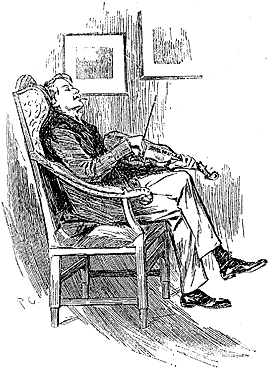
\includegraphics{images/study10-stud-03.png}\end{center}

\noindent \begin{center}\noun{Leaning back in his arm-chair of an
evening, he would close his eyes and scrape carelessly at the fiddle
which was thrown across his knee.}\end{center}
\end{figure}
Leaning back in his arm-chair of an evening, he would close his eyes
and scrape carelessly at the fiddle which was thrown across his knee.
Sometimes the chords were sonorous and melancholy. Occasionally they
were fantastic and cheerful. Clearly they reflected the thoughts which
possessed him, but whether the music aided those thoughts, or whether
the playing was simply the result of a whim or fancy was more than
I could determine. I might have rebelled against these exasperating
solos had it not been that he usually terminated them by playing in
quick succession a whole series of my favourite airs as a slight compensation
for the trial upon my patience.

During the first week or so we had no callers, and I had begun to
think that my companion was as friendless a man as I was myself. Presently,
however, I found that he had many acquaintances, and those in the
most different classes of society. There was one little sallow rat-faced,
dark-eyed fellow who was introduced to me as Mr.\ Lestrade, and who
came three or four times in a single week. One morning a young girl
called, fashionably dressed, and stayed for half an hour or more.
The same afternoon brought a grey-headed, seedy visitor, looking like
a Jew pedlar, who appeared to me to be much excited, and who was closely
followed by a slip-shod elderly woman. On another occasion an old
white-haired gentleman had an interview with my companion; and on
another a railway porter in his velveteen uniform. When any of these
nondescript individuals put in an appearance, Sherlock Holmes used
to beg for the use of the sitting-room, and I would retire to my bed-room.
He always apologized to me for putting me to this inconvenience. {}``I
have to use this room as a place of business,'' he said, {}``and
these people are my clients.'' Again I had an opportunity of asking
him a point blank question, and again my delicacy prevented me from
forcing another man to confide in me. I imagined at the time that
he had some strong reason for not alluding to it, but he soon dispelled
the idea by coming round to the subject of his own accord.

It was upon the 4th of March, as I have good reason to remember, that
I rose somewhat earlier than usual, and found that Sherlock Holmes
had not yet finished his breakfast. The landlady had become so accustomed
to my late habits that my place had not been laid nor my coffee prepared.
With the unreasonable petulance of mankind I rang the bell and gave
a curt intimation that I was ready. Then I picked up a magazine from
the table and attempted to while away the time with it, while my companion
munched silently at his toast. One of the articles had a pencil mark
at the heading, and I naturally began to run my eye through it.

Its somewhat ambitious title was {}``The Book of Life,'' and it
attempted to show how much an observant man might learn by an accurate
and systematic examination of all that came in his way. It struck
me as being a remarkable mixture of shrewdness and of absurdity. The
reasoning was close and intense, but the deductions appeared to me
to be far-fetched and exaggerated. The writer claimed by a momentary
expression, a twitch of a muscle or a glance of an eye, to fathom
a man's inmost thoughts. Deceit, according to him, was an impossibility
in the case of one trained to observation and analysis. His conclusions
were as infallible as so many propositions of Euclid. So startling
would his results appear to the uninitiated that until they learned
the processes by which he had arrived at them they might well consider
him as a necromancer.

{}``From a drop of water,'' said the writer, {}``a logician could
infer the possibility of an Atlantic or a Niagara without having seen
or heard of one or the other. So all life is a great chain, the nature
of which is known whenever we are shown a single link of it. Like
all other arts, the Science of Deduction and Analysis is one which
can only be acquired by long and patient study nor is life long enough
to allow any mortal to attain the highest possible perfection in it.
Before turning to those moral and mental aspects of the matter which
present the greatest difficulties, let the enquirer begin by mastering
more elementary problems. Let him, on meeting a fellow-mortal, learn
at a glance to distinguish the history of the man, and the trade or
profession to which he belongs. Puerile as such an exercise may seem,
it sharpens the faculties of observation, and teaches one where to
look and what to look for. By a man's finger nails, by his coat-sleeve,
by his boot, by his trouser knees, by the callosities of his forefinger
and thumb, by his expression, by his shirt cuffs\mdsh{---}by each
of these things a man's calling is plainly revealed. That all united
should fail to enlighten the competent enquirer in any case is almost
inconceivable.''

{}``What ineffable twaddle!'' I cried, slapping the magazine down
on the table, {}``I never read such rubbish in my life.''

{}``What is it?'' asked Sherlock Holmes.

{}``Why, this article,'' I said, pointing at it with my egg spoon
as I sat down to my breakfast. {}``I see that you have read it since
you have marked it. I don't deny that it is smartly written. It irritates
me though. It is evidently the theory of some arm-chair lounger who
evolves all these neat little paradoxes in the seclusion of his own
study. It is not practical. I should like to see him clapped down
in a third class carriage on the Underground, and asked to give the
trades of all his fellow-travellers. I would lay a thousand to one
against him.''

{}``You would lose your money,'' Sherlock Holmes remarked calmly.
{}``As for the article I wrote it myself.''

{}``You!''

{}``Yes, I have a turn both for observation and for deduction. The
theories which I have expressed there, and which appear to you to
be so chimerical are really extremely practical\mdsh{---}so practical
that I depend upon them for my bread and cheese.''

{}``And how?'' I asked involuntarily.

{}``Well, I have a trade of my own. I suppose I am the only one in
the world. I'm a consulting detective, if you can understand what
that is. Here in London we have lots of Government detectives and
lots of private ones. When these fellows are at fault they come to
me, and I manage to put them on the right scent. They lay all the
evidence before me, and I am generally able, by the help of my knowledge
of the history of crime, to set them straight. There is a strong family
resemblance about misdeeds, and if you have all the details of a thousand
at your finger ends, it is odd if you can't unravel the thousand and
first. Lestrade is a well-known detective. He got himself into a fog
recently over a forgery case, and that was what brought him here.''

{}``And these other people?''

{}``They are mostly sent on by private inquiry agencies. They are
all people who are in trouble about something, and want a little enlightening.
I listen to their story, they listen to my comments, and then I pocket
my fee.''

{}``But do you mean to say,'' I said, {}``that without leaving
your room you can unravel some knot which other men can make nothing
of, although they have seen every detail for themselves?''

{}``Quite so. I have a kind of intuition that way. Now and again
a case turns up which is a little more complex. Then I have to bustle
about and see things with my own eyes. You see I have a lot of special
knowledge which I apply to the problem, and which facilitates matters
wonderfully. Those rules of deduction laid down in that article which
aroused your scorn, are invaluable to me in practical work. Observation
with me is second nature. You appeared to be surprised when I told
you, on our first meeting, that you had come from Afghanistan.''

{}``You were told, no doubt.''

{}``Nothing of the sort. I \textit{knew} you came from Afghanistan.
From long habit the train of thoughts ran so swiftly through my mind,
that I arrived at the conclusion without being conscious of intermediate
steps. There were such steps, however. The train of reasoning ran,
`Here is a gentleman of a medical type, but with the air of a military
man. Clearly an army doctor, then. He has just come from the tropics,
for his face is dark, and that is not the natural tint of his skin,
for his wrists are fair. He has undergone hardship and sickness, as
his haggard face says clearly. His left arm has been injured. He holds
it in a stiff and unnatural manner. Where in the tropics could an
English army doctor have seen much hardship and got his arm wounded?
Clearly in Afghanistan.' The whole train of thought did not occupy
a second. I then remarked that you came from Afghanistan, and you
were astonished.''

{}``It is simple enough as you explain it,'' I said, smiling. {}``You
remind me of Edgar Allen Poe's Dupin. I had no idea that such individuals
did exist outside of stories.''

Sherlock Holmes rose and lit his pipe. {}``No doubt you think that
you are complimenting me in comparing me to Dupin,'' he observed.
{}``Now, in my opinion, Dupin was a very inferior fellow. That trick
of his of breaking in on his friends' thoughts with an apropos remark
after a quarter of an hour's silence is really very showy and superficial.
He had some analytical genius, no doubt; but he was by no means such
a phenomenon as Poe appeared to imagine.''

{}``Have you read Gaboriau's works?'' I asked. {}``Does Lecoq come
up to your idea of a detective?''

Sherlock Holmes sniffed sardonically. {}``Lecoq was a miserable bungler,''
he said, in an angry voice; {}``he had only one thing to recommend
him, and that was his energy. That book made me positively ill. The
question was how to identify an unknown prisoner. I could have done
it in twenty-four hours. Lecoq took six months or so. It might be
made a text-book for detectives to teach them what to avoid.''

I felt rather indignant at having two characters whom I had admired
treated in this cavalier style. I walked over to the window, and stood
looking out into the busy street. {}``This fellow may be very clever,''
I said to myself, {}``but he is certainly very conceited.''

{}``There are no crimes and no criminals in these days,'' he said,
querulously. {}``What is the use of having brains in our profession.
I know well that I have it in me to make my name famous. No man lives
or has ever lived who has brought the same amount of study and of
natural talent to the detection of crime which I have done. And what
is the result? There is no crime to detect, or, at most, some bungling
villany with a motive so transparent that even a Scotland Yard official
can see through it.''

I was still annoyed at his bumptious style of conversation. I thought
it best to change the topic.

{}``I wonder what that fellow is looking for?''\ I asked, pointing
to a stalwart, plainly-dressed individual who was walking slowly down
the other side of the street, looking anxiously at the numbers. He
had a large blue envelope in his hand, and was evidently the bearer
of a message.

{}``You mean the retired sergeant of Marines,'' said Sherlock Holmes.

{}``Brag and bounce!''\ thought I to myself. {}``He knows that
I cannot verify his guess.''

The thought had hardly passed through my mind when the man whom we
were watching caught sight of the number on our door, and ran rapidly
across the roadway. We heard a loud knock, a deep voice below, and
heavy steps ascending the stair.

%
\begin{figure}[htbp]
\noindent \begin{center}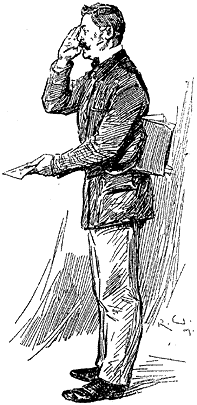
\includegraphics{images/study10-stud-04.png}\end{center}

\noindent \begin{center}\noun{{}``For Mr.\ Sherlock Holmes,''
he said.}\end{center}
\end{figure}
{}``For Mr.\ Sherlock Holmes,'' he said, stepping into the room
and handing my friend the letter.

Here was an opportunity of taking the conceit out of him. He little
thought of this when he made that random shot. {}``May I ask, my
lad,'' I said, in the blandest voice, {}``what your trade may be?''

{}``Commissionaire, sir,'' he said, gruffly. {}``Uniform away for
repairs.''

{}``And you were?'' I asked, with a slightly malicious glance at
my companion.

{}``A sergeant, sir, Royal Marine Light Infantry, sir. No answer?
Right, sir.''

He clicked his heels together, raised his hand in a salute, and was
gone.


\chapter*{\raggedright CHAPTER III. THE LAURISTON GARDEN MYSTERY}

\addcontentsline{toc}{chapter}{CHAPTER III. THE LAURISTON\\
GARDEN MYSTERY}

\markboth{A STUDY IN SCARLET}{CHAPTER III}

I confess that I was considerably startled by this fresh proof of
the practical nature of my companion's theories. My respect for his
powers of analysis increased wondrously. There still remained some
lurking suspicion in my mind, however, that the whole thing was a
pre-arranged episode, intended to dazzle me, though what earthly object
he could have in taking me in was past my comprehension. When I looked
at him he had finished reading the note, and his eyes had assumed
the vacant, lack-lustre expression which showed mental abstraction.

{}``How in the world did you deduce that?'' I asked.

{}``Deduce what?'' said he, petulantly.

{}``Why, that he was a retired sergeant of Marines.''

{}``I have no time for trifles,'' he answered, brusquely; then with
a smile, {}``Excuse my rudeness. You broke the thread of my thoughts;
but perhaps it is as well. So you actually were not able to see that
that man was a sergeant of Marines?''

{}``No, indeed.''

{}``It was easier to know it than to explain why I knew it. If you
were asked to prove that two and two made four, you might find some
difficulty, and yet you are quite sure of the fact. Even across the
street I could see a great blue anchor tattooed on the back of the
fellow's hand. That smacked of the sea. He had a military carriage,
however, and regulation side whiskers. There we have the marine. He
was a man with some amount of self-importance and a certain air of
command. You must have observed the way in which he held his head
and swung his cane. A steady, respectable, middle-aged man, too, on
the face of him\mdsh{---}all facts which led me to believe that he
had been a sergeant.''

{}``Wonderful!'' I ejaculated.

{}``Commonplace,'' said Holmes, though I thought from his expression
that he was pleased at my evident surprise and admiration. {}``I
said just now that there were no criminals. It appears that I am wrong\mdsh{---}look
at this!'' He threw me over the note which the commissionaire had
brought.

{}``Why,'' I cried, as I cast my eye over it, {}``this is terrible!''

{}``It does seem to be a little out of the common,'' he remarked,
calmly. {}``Would you mind reading it to me aloud?''

This is the letter which I read to him\mdsh{---}

\begin{quotation}
\noindent {}``\noun{My dear }\\
\noun{Mr.\ Sherlock Holmes},\mdsh{---}

{}``There has been a bad business during the night at 3, Lauriston
Gardens, off the Brixton Road. Our man on the beat saw a light there
about two in the morning, and as the house was an empty one, suspected
that something was amiss. He found the door open, and in the front
room, which is bare of furniture, discovered the body of a gentleman,
well dressed, and having cards in his pocket bearing the name of `Enoch
J.\ Drebber, Cleveland, Ohio, U.S.A.' There had been no robbery,
nor is there any evidence as to how the man met his death. There are
marks of blood in the room, but there is no wound upon his person.
We are at a loss as to how he came into the empty house; indeed, the
whole affair is a puzzler. If you can come round to the house any
time before twelve, you will find me there. I have left everything
\textit{in statu quo} until I hear from you. If you are unable to
come I shall give you fuller details, and would esteem it a great
kindness if you would favour me with your opinion. Yours faithfully, 

\begin{flushright}{}``\noun{Tobias Gregson}.''\end{flushright}
\end{quotation}
{}``Gregson is the smartest of the Scotland Yarders,'' my friend
remarked; {}``he and Lestrade are the pick of a bad lot. They are
both quick and energetic, but conventional\mdsh{---}shockingly so.
They have their knives into one another, too. They are as jealous
as a pair of professional beauties. There will be some fun over this
case if they are both put upon the scent.''

I was amazed at the calm way in which he rippled on. {}``Surely there
is not a moment to be lost,'' I cried, {}``shall I go and order
you a cab?''

{}``I'm not sure about whether I shall go. I am the most incurably
lazy devil that ever stood in shoe leather\mdsh{---}that is, when
the fit is on me, for I can be spry enough at times.''

{}``Why, it is just such a chance as you have been longing for.''

{}``My dear fellow, what does it matter to me. Supposing I unravel
the whole matter, you may be sure that Gregson, Lestrade, and Co.\ will
pocket all the credit. That comes of being an unofficial personage.''

{}``But he begs you to help him.''

{}``Yes. He knows that I am his superior, and acknowledges it to
me; but he would cut his tongue out before he would own it to any
third person. However, we may as well go and have a look. I shall
work it out on my own hook. I may have a laugh at them if I have nothing
else. Come on!''

He hustled on his overcoat, and bustled about in a way that showed
that an energetic fit had superseded the apathetic one.

{}``Get your hat,'' he said.

{}``You wish me to come?''

{}``Yes, if you have nothing better to do.'' A minute later we were
both in a hansom, driving furiously for the Brixton Road.

It was a foggy, cloudy morning, and a dun-coloured veil hung over
the house-tops, looking like the reflection of the mud-coloured streets
beneath. My companion was in the best of spirits, and prattled away
about Cremona fiddles, and the difference between a Stradivarius and
an Amati. As for myself, I was silent, for the dull weather and the
melancholy business upon which we were engaged, depressed my spirits.

{}``You don't seem to give much thought to the matter in hand,''
I said at last, interrupting Holmes' musical disquisition.

{}``No data yet,'' he answered. {}``It is a capital mistake to
theorize before you have all the evidence. It biases the judgment.''

{}``You will have your data soon,'' I remarked, pointing with my
finger; {}``this is the Brixton Road, and that is the house, if I
am not very much mistaken.''

{}``So it is. Stop, driver, stop!'' We were still a hundred yards
or so from it, but he insisted upon our alighting, and we finished
our journey upon foot.

Number 3, Lauriston Gardens wore an ill-omened and minatory look.
It was one of four which stood back some little way from the street,
two being occupied and two empty. The latter looked out with three
tiers of vacant melancholy windows, which were blank and dreary, save
that here and there a {}``To Let'' card had developed like a cataract
upon the bleared panes. A small garden sprinkled over with a scattered
eruption of sickly plants separated each of these houses from the
street, and was traversed by a narrow pathway, yellowish in colour,
and consisting apparently of a mixture of clay and of gravel. The
whole place was very sloppy from the rain which had fallen through
the night. The garden was bounded by a three-foot brick wall with
a fringe of wood rails upon the top, and against this wall was leaning
a stalwart police constable, surrounded by a small knot of loafers,
who craned their necks and strained their eyes in the vain hope of
catching some glimpse of the proceedings within.

I had imagined that Sherlock Holmes would at once have hurried into
the house and plunged into a study of the mystery. Nothing appeared
to be further from his intention. With an air of nonchalance which,
under the circumstances, seemed to me to border upon affectation,
he lounged up and down the pavement, and gazed vacantly at the ground,
the sky, the opposite houses and the line of railings. Having finished
his scrutiny, he proceeded slowly down the path, or rather down the
fringe of grass which flanked the path, keeping his eyes riveted upon
the ground. Twice he stopped, and once I saw him smile, and heard
him utter an exclamation of satisfaction. There were many marks of
footsteps upon the wet clayey soil, but since the police had been
coming and going over it, I was unable to see how my companion could
hope to learn anything from it. Still I had had such extraordinary
evidence of the quickness of his perceptive faculties, that I had
no doubt that he could see a great deal which was hidden from me.

At the door of the house we were met by a tall, white-faced, flaxen-haired
man, with a notebook in his hand, who rushed forward and wrung my
companion's hand with effusion. {}``It is indeed kind of you to come,''
he said, {}``I have had everything left untouched.''

{}``Except that!'' my friend answered, pointing at the pathway.
{}``If a herd of buffaloes had passed along there could not be a
greater mess. No doubt, however, you had drawn your own conclusions,
Gregson, before you permitted this.''

{}``I have had so much to do inside the house,'' the detective said
evasively. {}``My colleague, Mr.\ Lestrade, is here. I had relied
upon him to look after this.''

Holmes glanced at me and raised his eyebrows sardonically. {}``With
two such men as yourself and Lestrade upon the ground, there will
not be much for a third party to find out,'' he said.

Gregson rubbed his hands in a self-satisfied way. {}``I think we
have done all that can be done,'' he answered; {}``it's a queer
case though, and I knew your taste for such things.''

{}``You did not come here in a cab?'' asked Sherlock Holmes.

{}``No, sir.''

{}``Nor Lestrade?''

{}``No, sir.''

{}``Then let us go and look at the room.'' With which inconsequent
remark he strode on into the house, followed by Gregson, whose features
expressed his astonishment.

A short passage, bare planked and dusty, led to the kitchen and offices.
Two doors opened out of it to the left and to the right. One of these
had obviously been closed for many weeks. The other belonged to the
dining-room, which was the apartment in which the mysterious affair
had occurred. Holmes walked in, and I followed him with that subdued
feeling at my heart which the presence of death inspires.

It was a large square room, looking all the larger from the absence
of all furniture. A vulgar flaring paper adorned the walls, but it
was blotched in places with mildew, and here and there great strips
had become detached and hung down, exposing the yellow plaster beneath.
Opposite the door was a showy fireplace, surmounted by a mantelpiece
of imitation white marble. On one corner of this was stuck the stump
of a red wax candle. The solitary window was so dirty that the light
was hazy and uncertain, giving a dull grey tinge to everything, which
was intensified by the thick layer of dust which coated the whole
apartment.

%
\begin{figure}[htbp]
\noindent \begin{center}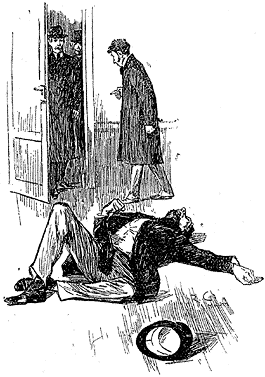
\includegraphics{images/study10-stud-05.png}\end{center}

\noindent \begin{center}\noun{My attention was centred upon the
single grim motionless figure which lay stretched upon the boards.}\end{center}
\end{figure}
All these details I observed afterwards. At present my attention was
centred upon the single grim motionless figure which lay stretched
upon the boards, with vacant sightless eyes staring up at the discoloured
ceiling. It was that of a man about forty-three or forty-four years
of age, middle-sized, broad shouldered, with crisp curling black hair,
and a short stubbly beard. He was dressed in a heavy broadcloth frock
coat and waistcoat, with light-coloured trousers, and immaculate collar
and cuffs. A top hat, well brushed and trim, was placed upon the floor
beside him. His hands were clenched and his arms thrown abroad, while
his lower limbs were interlocked as though his death struggle had
been a grievous one. On his rigid face there stood an expression of
horror, and as it seemed to me, of hatred, such as I have never seen
upon human features. This malignant and terrible contortion, combined
with the low forehead, blunt nose, and prognathous jaw gave the dead
man a singularly simious and ape-like appearance, which was increased
by his writhing, unnatural posture. I have seen death in many forms,
but never has it appeared to me in a more fearsome aspect than in
that dark grimy apartment, which looked out upon one of the main arteries
of suburban London.

Lestrade, lean and ferret-like as ever, was standing by the doorway,
and greeted my companion and myself.

{}``This case will make a stir, sir,'' he remarked. {}``It beats
anything I have seen, and I am no chicken.''

{}``There is no clue?''\ said Gregson.

{}``None at all,'' chimed in Lestrade.

Sherlock Holmes approached the body, and, kneeling down, examined
it intently. {}``You are sure that there is no wound?''\ he asked,
pointing to numerous gouts and splashes of blood which lay all round.

{}``Positive!''\ cried both detectives.

{}``Then, of course, this blood belongs to a second individual\mdsh{---}presumably
the murderer, if murder has been committed. It reminds me of the circumstances
attendant on the death of Van Jansen, in Utrecht, in the year '34.
Do you remember the case, Gregson?''

{}``No, sir.''

{}``Read it up\mdsh{---}you really should. There is nothing new
under the sun. It has all been done before.''

As he spoke, his nimble fingers were flying here, there, and everywhere,
feeling, pressing, unbuttoning, examining, while his eyes wore the
same far-away expression which I have already remarked upon. So swiftly
was the examination made, that one would hardly have guessed the minuteness
with which it was conducted. Finally, he sniffed the dead man's lips,
and then glanced at the soles of his patent leather boots.

{}``He has not been moved at all?''\ he asked.

{}``No more than was necessary for the purposes of our examination.''

{}``You can take him to the mortuary now,'' he said. {}``There
is nothing more to be learned.''

Gregson had a stretcher and four men at hand. At his call they entered
the room, and the stranger was lifted and carried out. As they raised
him, a ring tinkled down and rolled across the floor. Lestrade grabbed
it up and stared at it with mystified eyes.

{}``There's been a woman here,'' he cried. {}``It's a woman's wedding-ring.''

He held it out, as he spoke, upon the palm of his hand. We all gathered
round him and gazed at it. There could be no doubt that that circlet
of plain gold had once adorned the finger of a bride.

{}``This complicates matters,'' said Gregson. {}``Heaven knows,
they were complicated enough before.''

{}``You're sure it doesn't simplify them?'' observed Holmes. {}``There's
nothing to be learned by staring at it. What did you find in his pockets?''

{}``We have it all here,'' said Gregson, pointing to a litter of
objects upon one of the bottom steps of the stairs. {}``A gold watch,
No.\ 97163, by Barraud, of London. Gold Albert chain, very heavy
and solid. Gold ring, with masonic device. Gold pin\mdsh{---}bull-dog's
head, with rubies as eyes. Russian leather card-case, with cards of
Enoch J.\ Drebber of Cleveland, corresponding with the E.\ J.\ D.\ upon
the linen. No purse, but loose money to the extent of seven pounds
thirteen. Pocket edition of Boccaccio's `Decameron,' with name of
Joseph Stangerson upon the fly-leaf. Two letters\mdsh{---}one addressed
to E.\ J.\ Drebber and one to Joseph Stangerson.''

{}``At what address?''

{}``American Exchange, Strand\mdsh{---}to be left till called for.
They are both from the Guion Steamship Company, and refer to the sailing
of their boats from Liverpool. It is clear that this unfortunate man
was about to return to New York.''

{}``Have you made any inquiries as to this man, Stangerson?''

{}``I did it at once, sir,'' said Gregson. {}``I have had advertisements
sent to all the newspapers, and one of my men has gone to the American
Exchange, but he has not returned yet.''

{}``Have you sent to Cleveland?''

{}``We telegraphed this morning.''

{}``How did you word your inquiries?''

{}``We simply detailed the circumstances, and said that we should
be glad of any information which could help us.''

{}``You did not ask for particulars on any point which appeared to
you to be crucial?''

{}``I asked about Stangerson.''

{}``Nothing else? Is there no circumstance on which this whole case
appears to hinge? Will you not telegraph again?''

{}``I have said all I have to say,'' said Gregson, in an offended
voice.

Sherlock Holmes chuckled to himself, and appeared to be about to make
some remark, when Lestrade, who had been in the front room while we
were holding this conversation in the hall, reappeared upon the scene,
rubbing his hands in a pompous and self-satisfied manner.

{}``Mr.\ Gregson,'' he said, {}``I have just made a discovery
of the highest importance, and one which would have been overlooked
had I not made a careful examination of the walls.''

The little man's eyes sparkled as he spoke, and he was evidently in
a state of suppressed exultation at having scored a point against
his colleague.

{}``Come here,'' he said, bustling back into the room, the atmosphere
of which felt clearer since the removal of its ghastly inmate. {}``Now,
stand there!''

He struck a match on his boot and held it up against the wall.

%
\begin{figure}[htbp]
\noindent \begin{center}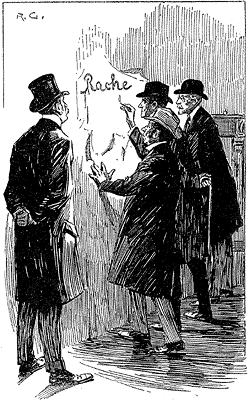
\includegraphics{images/study10-stud-06.png}\end{center}

\noindent \begin{center}\noun{{}``Look at that!'' he said, triumphantly.}\end{center}
\end{figure}
{}``Look at that!'' he said, triumphantly.

I have remarked that the paper had fallen away in parts. In this particular
corner of the room a large piece had peeled off, leaving a yellow
square of coarse plastering. Across this bare space there was scrawled
in blood-red letters a single word---

\noindent \begin{center}RACHE\end{center}

{}

{}``What do you think of that?'' cried the detective, with the air
of a showman exhibiting his show. {}``This was overlooked because
it was in the darkest corner of the room, and no one thought of looking
there. The murderer has written it with his or her own blood. See
this smear where it has trickled down the wall! That disposes of the
idea of suicide anyhow. Why was that corner chosen to write it on?
I will tell you. See that candle on the mantelpiece. It was lit at
the time, and if it was lit this corner would be the brightest instead
of the darkest portion of the wall.''

{}``And what does it mean now that you \textit{have} found it?''\ asked
Gregson in a depreciatory voice.

{}``Mean? Why, it means that the writer was going to put the female
name Rachel, but was disturbed before he or she had time to finish.
You mark my words, when this case comes to be cleared up you will
find that a woman named Rachel has something to do with it. It's all
very well for you to laugh, Mr.\ Sherlock Holmes. You may be very
smart and clever, but the old hound is the best, when all is said
and done.''

{}``I really beg your pardon!''\ said my companion, who had ruffled
the little man's temper by bursting into an explosion of laughter.
{}``You certainly have the credit of being the first of us to find
this out, and, as you say, it bears every mark of having been written
by the other participant in last night's mystery. I have not had time
to examine this room yet, but with your permission I shall do so now.''

As he spoke, he whipped a tape measure and a large round magnifying
glass from his pocket. With these two implements he trotted noiselessly
about the room, sometimes stopping, occasionally kneeling, and once
lying flat upon his face. So engrossed was he with his occupation
that he appeared to have forgotten our presence, for he chattered
away to himself under his breath the whole time, keeping up a running
fire of exclamations, groans, whistles, and little cries suggestive
of encouragement and of hope. As I watched him I was irresistibly
reminded of a pure-blooded well-trained foxhound as it dashes backwards
and forwards through the covert, whining in its eagerness, until it
comes across the lost scent. For twenty minutes or more he continued
his researches, measuring with the most exact care the distance between
marks which were entirely invisible to me, and occasionally applying
his tape to the walls in an equally incomprehensible manner. In one
place he gathered up very carefully a little pile of grey dust from
the floor, and packed it away in an envelope. Finally, he examined
with his glass the word upon the wall, going over every letter of
it with the most minute exactness. This done, he appeared to be satisfied,
for he replaced his tape and his glass in his pocket.

{}``They say that genius is an infinite capacity for taking pains,''
he remarked with a smile. {}``It's a very bad definition, but it
does apply to detective work.''

Gregson and Lestrade had watched the man\oe uvres of their amateur
companion with considerable curiosity and some contempt. They evidently
failed to appreciate the fact, which I had begun to realize, that
Sherlock Holmes' smallest actions were all directed towards some definite
and practical end.

{}``What do you think of it, sir?'' they both asked.

{}``It would be robbing you of the credit of the case if I was to
presume to help you,'' remarked my friend. {}``You are doing so
well now that it would be a pity for anyone to interfere.'' There
was a world of sarcasm in his voice as he spoke. {}``If you will
let me know how your investigations go,'' he continued, {}``I shall
be happy to give you any help I can. In the meantime I should like
to speak to the constable who found the body. Can you give me his
name and address?''

Lestrade glanced at his note-book. {}``John Rance,'' he said. {}``He
is off duty now. You will find him at 46, Audley Court, Kennington
Park Gate.''

Holmes took a note of the address.

{}``Come along, Doctor,'' he said; {}``we shall go and look him
up. I'll tell you one thing which may help you in the case,'' he
continued, turning to the two detectives. {}``There has been murder
done, and the murderer was a man. He was more than six feet high,
was in the prime of life, had small feet for his height, wore coarse,
square-toed boots and smoked a Trichinopoly cigar. He came here with
his victim in a four-wheeled cab, which was drawn by a horse with
three old shoes and one new one on his off fore leg. In all probability
the murderer had a florid face, and the finger-nails of his right
hand were remarkably long. These are only a few indications, but they
may assist you.''

Lestrade and Gregson glanced at each other with an incredulous smile.

{}``If this man was murdered, how was it done?'' asked the former.

{}``Poison,'' said Sherlock Holmes curtly, and strode off. {}``One
other thing, Lestrade,'' he added, turning round at the door: {}```Rache,'
is the German for `revenge;' so don't lose your time looking for Miss
Rachel.''

With which Parthian shot he walked away, leaving the two rivals open-mouthed
behind him.


\chapter*{\raggedright CHAPTER IV. WHAT JOHN RANCE HAD TO TELL.}

\addcontentsline{toc}{chapter}{CHAPTER IV. WHAT JOHN RANCE HAD\\
TO TELL.}

\markboth{A STUDY IN SCARLET}{CHAPTER IV}

It was one o'clock when we left No.\ 3, Lauriston Gardens. Sherlock
Holmes led me to the nearest telegraph office, whence he dispatched
a long telegram. He then hailed a cab, and ordered the driver to take
us to the address given us by Lestrade.

{}``There is nothing like first hand evidence,'' he remarked; {}``as
a matter of fact, my mind is entirely made up upon the case, but still
we may as well learn all that is to be learned.''

{}``You amaze me, Holmes,'' said I. {}``Surely you are not as sure
as you pretend to be of all those particulars which you gave.''

{}``There's no room for a mistake,'' he answered. {}``The very
first thing which I observed on arriving there was that a cab had
made two ruts with its wheels close to the curb. Now, up to last night,
we have had no rain for a week, so that those wheels which left such
a deep impression must have been there during the night. There were
the marks of the horse's hoofs, too, the outline of one of which was
far more clearly cut than that of the other three, showing that that
was a new shoe. Since the cab was there after the rain began, and
was not there at any time during the morning\mdsh{---}I have Gregson's
word for that\mdsh{---}it follows that it must have been there during
the night, and, therefore, that it brought those two individuals to
the house.''

{}``That seems simple enough,'' said I; {}``but how about the other
man's height?''

{}``Why, the height of a man, in nine cases out of ten, can be told
from the length of his stride. It is a simple calculation enough,
though there is no use my boring you with figures. I had this fellow's
stride both on the clay outside and on the dust within. Then I had
a way of checking my calculation. When a man writes on a wall, his
instinct leads him to write about the level of his own eyes. Now that
writing was just over six feet from the ground. It was child's play.''

{}``And his age?'' I asked.

{}``Well, if a man can stride four and a-half feet without the smallest
effort, he can't be quite in the sere and yellow. That was the breadth
of a puddle on the garden walk which he had evidently walked across.
Patent-leather boots had gone round, and Square-toes had hopped over.
There is no mystery about it at all. I am simply applying to ordinary
life a few of those precepts of observation and deduction which I
advocated in that article. Is there anything else that puzzles you?''

{}``The finger nails and the Trichinopoly,'' I suggested.

{}``The writing on the wall was done with a man's forefinger dipped
in blood. My glass allowed me to observe that the plaster was slightly
scratched in doing it, which would not have been the case if the man's
nail had been trimmed. I gathered up some scattered ash from the floor.
It was dark in colour and flakey\mdsh{---}such an ash as is only
made by a Trichinopoly. I have made a special study of cigar ashes\mdsh{---}in
fact, I have written a monograph upon the subject. I flatter myself
that I can distinguish at a glance the ash of any known brand, either
of cigar or of tobacco. It is just in such details that the skilled
detective differs from the Gregson and Lestrade type.''

{}``And the florid face?'' I asked.

{}``Ah, that was a more daring shot, though I have no doubt that
I was right. You must not ask me that at the present state of the
affair.''

I passed my hand over my brow. {}``My head is in a whirl,'' I remarked;
{}``the more one thinks of it the more mysterious it grows. How came
these two men\mdsh{---}if there were two men\mdsh{---}into an empty
house? What has become of the cabman who drove them? How could one
man compel another to take poison? Where did the blood come from?
What was the object of the murderer, since robbery had no part in
it? How came the woman's ring there? Above all, why should the second
man write up the German word RACHE before decamping? I confess that
I cannot see any possible way of reconciling all these facts.''

My companion smiled approvingly.

{}``You sum up the difficulties of the situation succinctly and well,''
he said. {}``There is much that is still obscure, though I have quite
made up my mind on the main facts. As to poor Lestrade's discovery
it was simply a blind intended to put the police upon a wrong track,
by suggesting Socialism and secret societies. It was not done by a
German. The A, if you noticed, was printed somewhat after the German
fashion. Now, a real German invariably prints in the Latin character,
so that we may safely say that this was not written by one, but by
a clumsy imitator who overdid his part. It was simply a ruse to divert
inquiry into a wrong channel. I'm not going to tell you much more
of the case, Doctor. You know a conjuror gets no credit when once
he has explained his trick, and if I show you too much of my method
of working, you will come to the conclusion that I am a very ordinary
individual after all.''

{}``I shall never do that,'' I answered; {}``you have brought detection
as near an exact science as it ever will be brought in this world.''

My companion flushed up with pleasure at my words, and the earnest
way in which I uttered them. I had already observed that he was as
sensitive to flattery on the score of his art as any girl could be
of her beauty.

{}``I'll tell you one other thing,'' he said. {}``Patent leathers
and Square-toes came in the same cab, and they walked down the pathway
together as friendly as possible\mdsh{---}arm-in-arm, in all probability.
When they got inside they walked up and down the room\mdsh{---}or
rather, Patent-leathers stood still while Square-toes walked up and
down. I could read all that in the dust; and I could read that as
he walked he grew more and more excited. That is shown by the increased
length of his strides. He was talking all the while, and working himself
up, no doubt, into a fury. Then the tragedy occurred. I've told you
all I know myself now, for the rest is mere surmise and conjecture.
We have a good working basis, however, on which to start. We must
hurry up, for I want to go to Halle's concert to hear Norman Neruda
this afternoon.''

This conversation had occurred while our cab had been threading its
way through a long succession of dingy streets and dreary by-ways.
In the dingiest and dreariest of them our driver suddenly came to
a stand. {}``That's Audley Court in there,'' he said, pointing to
a narrow slit in the line of dead-coloured brick. {}``You'll find
me here when you come back.''

%
\begin{figure}[htbp]
\noindent \begin{center}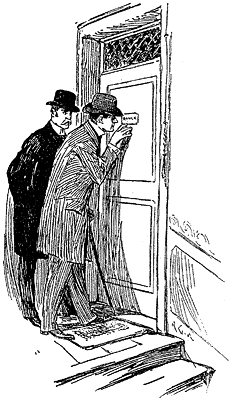
\includegraphics{images/study10-stud-07.png}\end{center}

\noindent \begin{center}\noun{The door was decorated with a small
slip of brass on which the name Rance was engraved.}\end{center}
\end{figure}
Audley Court was not an attractive locality. The narrow passage led
us into a quadrangle paved with flags and lined by sordid dwellings.
We picked our way among groups of dirty children, and through lines
of discoloured linen, until we came to Number 46, the door of which
was decorated with a small slip of brass on which the name Rance was
engraved. On enquiry we found that the constable was in bed, and we
were shown into a little front parlour to await his coming.

He appeared presently, looking a little irritable at being disturbed
in his slumbers. {}``I made my report at the office,'' he said.

Holmes took a half-sovereign from his pocket and played with it pensively.
{}``We thought that we should like to hear it all from your own lips,''
he said.

{}``I shall be most happy to tell you anything I can,'' the constable
answered with his eyes upon the little golden disk.

{}``Just let us hear it all in your own way as it occurred.''

Rance sat down on the horsehair sofa, and knitted his brows as though
determined not to omit anything in his narrative.

{}``I'll tell it ye from the beginning,'' he said. {}``My time
is from ten at night to six in the morning. At eleven there was a
fight at the `White Hart'; but bar that all was quiet enough on the
beat. At one o'clock it began to rain, and I met Harry Murcher\mdsh{---}him
who has the Holland Grove beat\mdsh{---}and we stood together at
the corner of Henrietta Street a-talkin'. Presently\mdsh{---}maybe
about two or a little after\mdsh{---}I thought I would take a look
round and see that all was right down the Brixton Road. It was precious
dirty and lonely. Not a soul did I meet all the way down, though a
cab or two went past me. I was a strollin' down, thinkin' between
ourselves how uncommon handy a four of gin hot would be, when suddenly
the glint of a light caught my eye in the window of that same house.
Now, I knew that them two houses in Lauriston Gardens was empty on
account of him that owns them who won't have the drains seed to, though
the very last tenant what lived in one of them died o' typhoid fever.
I was knocked all in a heap therefore at seeing a light in the window,
and I suspected as something was wrong. When I got to the door\mdsh{---}''

{}``You stopped, and then walked back to the garden gate,'' my companion
interrupted. {}``What did you do that for?''

Rance gave a violent jump, and stared at Sherlock Holmes with the
utmost amazement upon his features.

{}``Why, that's true, sir,'' he said; {}``though how you come to
know it, Heaven only knows. Ye see, when I got up to the door it was
so still and so lonesome, that I thought I'd be none the worse for
some one with me. I ain't afeared of anything on this side o' the
grave; but I thought that maybe it was him that died o' the typhoid
inspecting the drains what killed him. The thought gave me a kind
o' turn, and I walked back to the gate to see if I could see Murcher's
lantern, but there wasn't no sign of him nor of anyone else.''

{}``There was no one in the street?''

{}``Not a livin' soul, sir, nor as much as a dog. Then I pulled myself
together and went back and pushed the door open. All was quiet inside,
so I went into the room where the light was a-burnin'. There was a
candle flickerin' on the mantelpiece\mdsh{---}a red wax one\mdsh{---}and
by its light I saw\mdsh{---}''

{}``Yes, I know all that you saw. You walked round the room several
times, and you knelt down by the body, and then you walked through
and tried the kitchen door, and \mdsh{then\mdsh{---}''}

John Rance sprang to his feet with a frightened face and suspicion
in his eyes. {}``Where was you hid to see all that?''\ he cried.
{}``It seems to me that you knows a deal more than you should.''

Holmes laughed and threw his card across the table to the constable.
{}``Don't get arresting me for the murder,'' he said. {}``I am
one of the hounds and not the wolf; Mr.\ Gregson or Mr.\ Lestrade
will answer for that. Go on, though. What did you do next?''

Rance resumed his seat, without however losing his mystified expression.
{}``I went back to the gate and sounded my whistle. That brought
Murcher and two more to the spot.''

{}``Was the street empty then?''

{}``Well, it was, as far as anybody that could be of any good goes.''

{}``What do you mean?''

%
\begin{figure}[htbp]
\noindent \begin{center}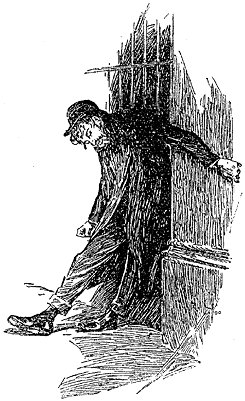
\includegraphics{images/study10-stud-08.png}\end{center}

\noindent \begin{center}\noun{{}``I've seen many a drunk chap in
my time,'' he said, {}``but never anyone so cryin' drunk as that
cove.''}\end{center}
\end{figure}
The constable's features broadened into a grin. {}``I've seen many
a drunk chap in my time,'' he said, {}``but never anyone so cryin'
drunk as that cove. He was at the gate when I came out, a-leanin'
up agin the railings, and a-singin' at the pitch o' his lungs about
Columbine's New-fangled Banner, or some such stuff. He couldn't stand,
far less help.''

{}``What sort of a man was he?'' asked Sherlock Holmes.

John Rance appeared to be somewhat irritated at this digression. {}``He
was an uncommon drunk sort o' man,'' he said. {}``He'd ha' found
hisself in the station if we hadn't been so took up.''

{}``His face\mdsh{---}his dress\mdsh{---}didn't you notice them?''
Holmes broke in impatiently.

{}``I should think I did notice them, seeing that I had to prop him
up\mdsh{---}me and Murcher between us. He was a long chap, with a
red face, the lower part muffled round\mdsh{---}''

{}``That will do,'' cried Holmes. {}``What became of him?''

{}``We'd enough to do without lookin' after him,'' the policeman
said, in an aggrieved voice. {}``I'll wager he found his way home
all right.''

{}``How was he dressed?''

{}``A brown overcoat.''

{}``Had he a whip in his hand?''

{}``A whip\mdsh{---}no.''

{}``He must have left it behind,'' muttered my companion. {}``You
didn't happen to see or hear a cab after that?''

{}``No.''

{}``There's a half-sovereign for you,'' my companion said, standing
up and taking his hat. {}``I am afraid, Rance, that you will never
rise in the force. That head of yours should be for use as well as
ornament. You might have gained your sergeant's stripes last night.
The man whom you held in your hands is the man who holds the clue
of this mystery, and whom we are seeking. There is no use of arguing
about it now; I tell you that it is so. Come along, Doctor.''

We started off for the cab together, leaving our informant incredulous,
but obviously uncomfortable.

{}``The blundering fool,'' Holmes said, bitterly, as we drove back
to our lodgings. {}``Just to think of his having such an incomparable
bit of good luck, and not taking advantage of it.''

{}``I am rather in the dark still. It is true that the description
of this man tallies with your idea of the second party in this mystery.
But why should he come back to the house after leaving it? That is
not the way of criminals.''

{}``The ring, man, the ring: that was what he came back for. If we
have no other way of catching him, we can always bait our line with
the ring. I shall have him, Doctor\mdsh{---}I'll lay you two to one
that I have him. I must thank you for it all. I might not have gone
but for you, and so have missed the finest study I ever came across:
a study in scarlet, eh? Why shouldn't we use a little art jargon.
There's the scarlet thread of murder running through the colourless
skein of life, and our duty is to unravel it, and isolate it, and
expose every inch of it. And now for lunch, and then for Norman Neruda.
Her attack and her bowing are splendid. What's that little thing of
Chopin's she plays so magnificently: Tra-la-la-lira-lira-lay.''

Leaning back in the cab, this amateur bloodhound carolled away like
a lark while I meditated upon the many-sidedness of the human mind.


\chapter*{\raggedright CHAPTER V. OUR ADVERTISEMENT BRINGS A VISITOR.}

\addcontentsline{toc}{chapter}{CHAPTER V. OUR ADVERTISEMENT\\
BRINGS A VISITOR.}

\markboth{A STUDY IN SCARLET}{CHAPTER V}

Our morning's exertions had been too much for my weak health, and
I was tired out in the afternoon. After Holmes' departure for the
concert, I lay down upon the sofa and endeavoured to get a couple
of hours' sleep. It was a useless attempt. My mind had been too much
excited by all that had occurred, and the strangest fancies and surmises
crowded into it. Every time that I closed my eyes I saw before me
the distorted baboon-like countenance of the murdered man. So sinister
was the impression which that face had produced upon me that I found
it difficult to feel anything but gratitude for him who had removed
its owner from the world. If ever human features bespoke vice of the
most malignant type, they were certainly those of Enoch J.\ Drebber,
of Cleveland. Still I recognized that justice must be done, and that
the depravity of the victim was no condonement in the eyes of the
law.

The more I thought of it the more extraordinary did my companion's
hypothesis, that the man had been poisoned, appear. I remembered how
he had sniffed his lips, and had no doubt that he had detected something
which had given rise to the idea. Then, again, if not poison, what
had caused the man's death, since there was neither wound nor marks
of strangulation? But, on the other hand, whose blood was that which
lay so thickly upon the floor? There were no signs of a struggle,
nor had the victim any weapon with which he might have wounded an
antagonist. As long as all these questions were unsolved, I felt that
sleep would be no easy matter, either for Holmes or myself. His quiet
self-confident manner convinced me that he had already formed a theory
which explained all the facts, though what it was I could not for
an instant conjecture.

He was very late in returning\mdsh{---}so late, that I knew that
the concert could not have detained him all the time. Dinner was on
the table before he appeared.

{}``It was magnificent,'' he said, as he took his seat. {}``Do
you remember what Darwin says about music? He claims that the power
of producing and appreciating it existed among the human race long
before the power of speech was arrived at. Perhaps that is why we
are so subtly influenced by it. There are vague memories in our souls
of those misty centuries when the world was in its childhood.''

{}``That's rather a broad idea,'' I remarked.

{}``One's ideas must be as broad as Nature if they are to interpret
Nature,'' he answered. {}``What's the matter? You're not looking
quite yourself. This Brixton Road affair has upset you.''

{}``To tell the truth, it has,'' I said. {}``I ought to be more
case-hardened after my Afghan experiences. I saw my own comrades hacked
to pieces at Maiwand without losing my nerve.''

{}``I can understand. There is a mystery about this which stimulates
the imagination; where there is no imagination there is no horror.
Have you seen the evening paper?''

{}``No.''

{}``It gives a fairly good account of the affair. It does not mention
the fact that when the man was raised up, a woman's wedding ring fell
upon the floor. It is just as well it does not.''

{}``Why?''

{}``Look at this advertisement,'' he answered. {}``I had one sent
to every paper this morning immediately after the affair.''

He threw the paper across to me and I glanced at the place indicated.
It was the first announcement in the {}``Found'' column. {}``In
Brixton Road, this morning,'' it ran, {}``a plain gold wedding ring,
found in the roadway between the `White Hart' Tavern and Holland Grove.
Apply Dr.\ Watson, \noun{221b}, Baker Street, between eight and
nine this evening.''

{}``Excuse my using your name,'' he said. {}``If I used my own
some of these dunderheads would recognize it, and want to meddle in
the affair.''

{}``That is all right,'' I answered. {}``But supposing anyone applies,
I have no ring.''

{}``Oh yes, you have,'' said he, handing me one. {}``This will
do very well. It is almost a facsimile.''

{}``And who do you expect will answer this advertisement.''

{}``Why, the man in the brown coat\mdsh{---}our florid friend with
the square toes. If he does not come himself he will send an accomplice.''

{}``Would he not consider it as too dangerous?''

{}``Not at all. If my view of the case is correct, and I have every
reason to believe that it is, this man would rather risk anything
than lose the ring. According to my notion he dropped it while stooping
over Drebber's body, and did not miss it at the time. After leaving
the house he discovered his loss and hurried back, but found the police
already in possession, owing to his own folly in leaving the candle
burning. He had to pretend to be drunk in order to allay the suspicions
which might have been aroused by his appearance at the gate. Now put
yourself in that man's place. On thinking the matter over, it must
have occurred to him that it was possible that he had lost the ring
in the road after leaving the house. What would he do, then? He would
eagerly look out for the evening papers in the hope of seeing it among
the articles found. His eye, of course, would light upon this. He
would be overjoyed. Why should he fear a trap? There would be no reason
in his eyes why the finding of the ring should be connected with the
murder. He would come. He will come. You shall see him within an hour?''

{}``And then?'' I asked.

{}``Oh, you can leave me to deal with him then. Have you any arms?''

{}``I have my old service revolver and a few cartridges.''

{}``You had better clean it and load it. He will be a desperate man,
and though I shall take him unawares, it is as well to be ready for
anything.''

I went to my bedroom and followed his advice. When I returned with
the pistol the table had been cleared, and Holmes was engaged in his
favourite occupation of scraping upon his violin.

{}``The plot thickens,'' he said, as I entered; {}``I have just
had an answer to my American telegram. My view of the case is the
correct one.''

{}``And that is?'' I asked eagerly.

{}``My fiddle would be the better for new strings,'' he remarked.
{}``Put your pistol in your pocket. When the fellow comes speak to
him in an ordinary way. Leave the rest to me. Don't frighten him by
looking at him too hard.''

{}``It is eight o'clock now,'' I said, glancing at my watch.

{}``Yes. He will probably be here in a few minutes. Open the door
slightly. That will do. Now put the key on the inside. Thank you!
This is a queer old book I picked up at a stall yesterday\mdsh{---}`De
Jure inter Gentes'\mdsh{---}published in Latin at Liege in the Lowlands,
in 1642. Charles' head was still firm on his shoulders when this little
brown-backed volume was struck off.''

{}``Who is the printer?''

{}``Philippe de Croy, whoever he may have been. On the fly-leaf,
in very faded ink, is written `Ex libris Guliolmi Whyte.' I wonder
who William Whyte was. Some pragmatical seventeenth century lawyer,
I suppose. His writing has a legal twist about it. Here comes our
man, I think.''

As he spoke there was a sharp ring at the bell. Sherlock Holmes rose
softly and moved his chair in the direction of the door. We heard
the servant pass along the hall, and the sharp click of the latch
as she opened it.

{}``Does Dr.\ Watson live here?'' asked a clear but rather harsh
voice. We could not hear the servant's reply, but the door closed,
and some one began to ascend the stairs. The footfall was an uncertain
and shuffling one. A look of surprise passed over the face of my companion
as he listened to it. It came slowly along the passage, and there
was a feeble tap at the door.

{}``Come in,'' I cried.

%
\begin{figure}[htbp]
\noindent \begin{center}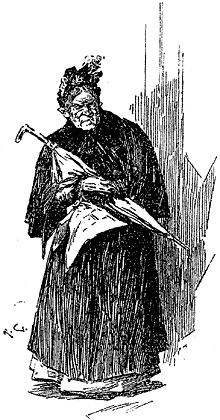
\includegraphics{images/study10-stud-09.png}\end{center}

\noindent \begin{center}\noun{A very old and wrinkled woman hobbled
into the apartment.}\end{center}
\end{figure}
At my summons, instead of the man of violence whom we expected, a
very old and wrinkled woman hobbled into the apartment. She appeared
to be dazzled by the sudden blaze of light, and after dropping a curtsey,
she stood blinking at us with her bleared eyes and fumbling in her
pocket with nervous, shaky fingers. I glanced at my companion, and
his face had assumed such a disconsolate expression that it was all
I could do to keep my countenance.

The old crone drew out an evening paper, and pointed at our advertisement.
{}``It's this as has brought me, good gentlemen,'' she said, dropping
another curtsey; {}``a gold wedding ring in the Brixton Road. It
belongs to my girl Sally, as was married only this time twelvemonth,
which her husband is steward aboard a Union boat, and what he'd say
if he come 'ome and found her without her ring is more than I can
think, he being short enough at the best o' times, but more especially
when he has the drink. If it please you, she went to the circus last
night along with\mdsh{---}''

{}``Is that her ring?''\ I asked.

{}``The Lord be thanked!''\ cried the old woman; {}``Sally will
be a glad woman this night. That's the ring.''

{}``And what may your address be?''\ I inquired, taking up a pencil.

{}``13, Duncan Street, Houndsditch. A weary way from here.''

{}``The Brixton Road does not lie between any circus and Houndsditch,''
said Sherlock Holmes sharply.

The old woman faced round and looked keenly at him from her little
red-rimmed eyes. {}``The gentleman asked me for \textit{my} address,''
she said. {}``Sally lives in lodgings at 3, Mayfield Place, Peckham.''

{}``And your name is\mdsh{---}?''

{}``My name is Sawyer\mdsh{---}her's is Dennis, which Tom Dennis
married her\mdsh{---}and a smart, clean lad, too, as long as he's
at sea, and no steward in the company more thought of; but when on
shore, what with the women and what with liquor shops\mdsh{---}''

{}``Here is your ring, Mrs.\ Sawyer,'' I interrupted, in obedience
to a sign from my companion; {}``it clearly belongs to your daughter,
and I am glad to be able to restore it to the rightful owner.''

With many mumbled blessings and protestations of gratitude the old
crone packed it away in her pocket, and shuffled off down the stairs.
Sherlock Holmes sprang to his feet the moment that she was gone and
rushed into his room. He returned in a few seconds enveloped in an
ulster and a cravat. {}``I'll follow her,'' he said, hurriedly;
{}``she must be an accomplice, and will lead me to him. Wait up for
me.'' The hall door had hardly slammed behind our visitor before
Holmes had descended the stair. Looking through the window I could
see her walking feebly along the other side, while her pursuer dogged
her some little distance behind. {}``Either his whole theory is incorrect,''
I thought to myself, {}``or else he will be led now to the heart
of the mystery.'' There was no need for him to ask me to wait up
for him, for I felt that sleep was impossible until I heard the result
of his adventure.

It was close upon nine when he set out. I had no idea how long he
might be, but I sat stolidly puffing at my pipe and skipping over
the pages of Henri Murger's {}``Vie de Boh�me.'' Ten o'clock passed,
and I heard the footsteps of the maid as they pattered off to bed.
Eleven, and the more stately tread of the landlady passed my door,
bound for the same destination. It was close upon twelve before I
heard the sharp sound of his latch-key. The instant he entered I saw
by his face that he had not been successful. Amusement and chagrin
seemed to be struggling for the mastery, until the former suddenly
carried the day, and he burst into a hearty laugh.

{}``I wouldn't have the Scotland Yarders know it for the world,''
he cried, dropping into his chair; {}``I have chaffed them so much
that they would never have let me hear the end of it. I can afford
to laugh, because I know that I will be even with them in the long
run.''

{}``What is it then?'' I asked.

{}``Oh, I don't mind telling a story against myself. That creature
had gone a little way when she began to limp and show every sign of
being foot-sore. Presently she came to a halt, and hailed a four-wheeler
which was passing. I managed to be close to her so as to hear the
address, but I need not have been so anxious, for she sang it out
loud enough to be heard at the other side of the street, `Drive to
13, Duncan Street, Houndsditch,' she cried. This begins to look genuine,
I thought, and having seen her safely inside, I perched myself behind.
That's an art which every detective should be an expert at. Well,
away we rattled, and never drew rein until we reached the street in
question. I hopped off before we came to the door, and strolled down
the street in an easy, lounging way. I saw the cab pull up. The driver
jumped down, and I saw him open the door and stand expectantly. Nothing
came out though. When I reached him he was groping about frantically
in the empty cab, and giving vent to the finest assorted collection
of oaths that ever I listened to. There was no sign or trace of his
passenger, and I fear it will be some time before he gets his fare.
On inquiring at Number 13 we found that the house belonged to a respectable
paperhanger, named Keswick, and that no one of the name either of
Sawyer or Dennis had ever been heard of there.''

{}``You don't mean to say,'' I cried, in amazement, {}``that that
tottering, feeble old woman was able to get out of the cab while it
was in motion, without either you or the driver seeing her?''

{}``Old woman be damned!'' said Sherlock Holmes, sharply. {}``We
were the old women to be so taken in. It must have been a young man,
and an active one, too, besides being an incomparable actor. The get-up
was inimitable. He saw that he was followed, no doubt, and used this
means of giving me the slip. It shows that the man we are after is
not as lonely as I imagined he was, but has friends who are ready
to risk something for him. Now, Doctor, you are looking done-up. Take
my advice and turn in.''

I was certainly feeling very weary, so I obeyed his injunction. I
left Holmes seated in front of the smouldering fire, and long into
the watches of the night I heard the low, melancholy wailings of his
violin, and knew that he was still pondering over the strange problem
which he had set himself to unravel.


\chapter*{\raggedright CHAPTER VI. TOBIAS GREGSON SHOWS WHAT HE CAN DO.}

\addcontentsline{toc}{chapter}{CHAPTER VI. TOBIAS GREGSON SHOWS\\
WHAT HE CAN DO.}

\markboth{A STUDY IN SCARLET}{CHAPTER VI}

The papers next day were full of the {}``Brixton Mystery,'' as they
termed it. Each had a long account of the affair, and some had leaders
upon it in addition. There was some information in them which was
new to me. I still retain in my scrap-book numerous clippings and
extracts bearing upon the case. Here is a condensation of a few of
them:\mdsh{---}

The \textit{Daily Telegraph} remarked that in the history of crime
there had seldom been a tragedy which presented stranger features.
The German name of the victim, the absence of all other motive, and
the sinister inscription on the wall, all pointed to its perpetration
by political refugees and revolutionists. The Socialists had many
branches in America, and the deceased had, no doubt, infringed their
unwritten laws, and been tracked down by them. After alluding airily
to the Vehmgericht, aqua tofana, Carbonari, the Marchioness de Brinvilliers,
the Darwinian theory, the principles of Malthus, and the Ratcliff
Highway murders, the article concluded by admonishing the Government
and advocating a closer watch over foreigners in England.

The \textit{Standard} commented upon the fact that lawless outrages
of the sort usually occurred under a Liberal Administration. They
arose from the unsettling of the minds of the masses, and the consequent
weakening of all authority. The deceased was an American gentleman
who had been residing for some weeks in the Metropolis. He had stayed
at the boarding-house of Madame Charpentier, in Torquay Terrace, Camberwell.
He was accompanied in his travels by his private secretary, Mr.\ Joseph
Stangerson. The two bade adieu to their landlady upon Tuesday, the
4th inst., and departed to Euston Station with the avowed intention
of catching the Liverpool express. They were afterwards seen together
upon the platform. Nothing more is known of them until Mr.\ Drebber's
body was, as recorded, discovered in an empty house in the Brixton
Road, many miles from Euston. How he came there, or how he met his
fate, are questions which are still involved in mystery. Nothing is
known of the whereabouts of Stangerson. We are glad to learn that
Mr.\ Lestrade and Mr.\ Gregson, of Scotland Yard, are both engaged
upon the case, and it is confidently anticipated that these well-known
officers will speedily throw light upon the matter.

The \textit{Daily News} observed that there was no doubt as to the
crime being a political one. The despotism and hatred of Liberalism
which animated the Continental Governments had had the effect of driving
to our shores a number of men who might have made excellent citizens
were they not soured by the recollection of all that they had undergone.
Among these men there was a stringent code of honour, any infringement
of which was punished by death. Every effort should be made to find
the secretary, Stangerson, and to ascertain some particulars of the
habits of the deceased. A great step had been gained by the discovery
of the address of the house at which he had boarded\mdsh{---}a result
which was entirely due to the acuteness and energy of Mr.\ Gregson
of Scotland Yard.

Sherlock Holmes and I read these notices over together at breakfast,
and they appeared to afford him considerable amusement.

{}``I told you that, whatever happened, Lestrade and Gregson would
be sure to score.''

{}``That depends on how it turns out.''

{}``Oh, bless you, it doesn't matter in the least. If the man is
caught, it will be \textit{on account} of their exertions; if he escapes,
it will be \textit{in spite} of their exertions. It's heads I win
and tails you lose. Whatever they do, they will have followers.\ 
`Un sot trouve toujours un plus sot qui l'admire.'''

{}``What on earth is this?'' I cried, for at this moment there came
the pattering of many steps in the hall and on the stairs, accompanied
by audible expressions of disgust upon the part of our landlady.

{}``It's the Baker Street division of the detective police force,''
said my companion, gravely; and as he spoke there rushed into the
room half a dozen of the dirtiest and most ragged street Arabs that
ever I clapped eyes on.

%
\begin{figure}[htbp]
\noindent \begin{center}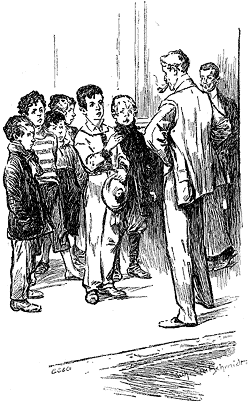
\includegraphics{images/study10-stud-10.png}\end{center}

\noindent \begin{center}\noun{{}``Have you found it, Wiggins?''}\end{center}
\end{figure}
{}``'Tention!'' cried Holmes, in a sharp tone, and the six dirty
little scoundrels stood in a line like so many disreputable statuettes.
{}``In future you shall send up Wiggins alone to report, and the
rest of you must wait in the street. Have you found it, Wiggins?''

{}``No, sir, we hain't,'' said one of the youths.

{}``I hardly expected you would. You must keep on until you do. Here
are your wages.'' He handed each of them a shilling. {}``Now, off
you go, and come back with a better report next time.''

He waved his hand, and they scampered away downstairs like so many
rats, and we heard their shrill voices next moment in the street.

{}``There's more work to be got out of one of those little beggars
than out of a dozen of the force,'' Holmes remarked. {}``The mere
sight of an official-looking person seals men's lips. These youngsters,
however, go everywhere and hear everything. They are as sharp as needles,
too; all they want is organisation.''

{}``Is it on this Brixton case that you are employing them?'' I
asked.

{}``Yes; there is a point which I wish to ascertain. It is merely
a matter of time. Hullo! we are going to hear some news now with a
vengeance! Here is Gregson coming down the road with beatitude written
upon every feature of his face. Bound for us, I know. Yes, he is stopping.
There he is!''

There was a violent peal at the bell, and in a few seconds the fair-haired
detective came up the stairs, three steps at a time, and burst into
our sitting-room.

{}``My dear fellow,'' he cried, wringing Holmes' unresponsive hand,
{}``congratulate me! I have made the whole thing as clear as day.''

A shade of anxiety seemed to me to cross my companion's expressive
face.

{}``Do you mean that you are on the right track?'' he asked.

{}``The right track! Why, sir, we have the man under lock and key.''

{}``And his name is?''

{}``Arthur Charpentier, sub-lieutenant in Her Majesty's navy,''
cried Gregson, pompously, rubbing his fat hands and inflating his
chest.

Sherlock Holmes gave a sigh of relief, and relaxed into a smile.

{}``Take a seat, and try one of these cigars,'' he said. {}``We
are anxious to know how you managed it. Will you have some whiskey
and water?''

{}``I don't mind if I do,'' the detective answered. {}``The tremendous
exertions which I have gone through during the last day or two have
worn me out. Not so much bodily exertion, you understand, as the strain
upon the mind. You will appreciate that, Mr.\ Sherlock Holmes, for
we are both brain-workers.''

{}``You do me too much honour,'' said Holmes, gravely. {}``Let
us hear how you arrived at this most gratifying result.''

The detective seated himself in the arm-chair, and puffed complacently
at his cigar. Then suddenly he slapped his thigh in a paroxysm of
amusement.

{}``The fun of it is,'' he cried, {}``that that fool Lestrade,
who thinks himself so smart, has gone off upon the wrong track altogether.
He is after the secretary Stangerson, who had no more to do with the
crime than the babe unborn. I have no doubt that he has caught him
by this time.''

The idea tickled Gregson so much that he laughed until he choked.

{}``And how did you get your clue?''

{}``Ah, I'll tell you all about it. Of course, Doctor Watson, this
is strictly between ourselves. The first difficulty which we had to
contend with was the finding of this American's antecedents. Some
people would have waited until their advertisements were answered,
or until parties came forward and volunteered information. That is
not Tobias Gregson's way of going to work. You remember the hat beside
the dead man?''

{}``Yes,'' said Holmes; {}``by John Underwood and Sons, 129, Camberwell
Road.''

Gregson looked quite crest-fallen.

{}``I had no idea that you noticed that,'' he said. {}``Have you
been there?''

{}``No.''

{}``Ha!''\ cried Gregson, in a relieved voice; {}``you should
never neglect a chance, however small it may seem.''

{}``To a great mind, nothing is little,'' remarked Holmes, sententiously.

{}``Well, I went to Underwood, and asked him if he had sold a hat
of that size and description. He looked over his books, and came on
it at once. He had sent the hat to a Mr.\ Drebber, residing at Charpentier's
Boarding Establishment, Torquay Terrace. Thus I got at his address.''

{}``Smart\mdsh{---}very smart!''\ murmured Sherlock Holmes.

{}``I next called upon Madame Charpentier,'' continued the detective.
{}``I found her very pale and distressed. Her daughter was in the
room, too\mdsh{---}an uncommonly fine girl she is, too; she was looking
red about the eyes and her lips trembled as I spoke to her. That didn't
escape my notice. I began to smell a rat. You know the feeling, Mr.\ Sherlock
Holmes, when you come upon the right scent\mdsh{---}a kind of thrill
in your nerves.\  `Have you heard of the mysterious death of your
late boarder Mr.\ Enoch J.\ Drebber, of Cleveland?' I asked.

{}``The mother nodded. She didn't seem able to get out a word. The
daughter burst into tears. I felt more than ever that these people
knew something of the matter.

{}```At what o'clock did Mr.\ Drebber leave your house for the train?'
I asked.

{}```At eight o'clock,' she said, gulping in her throat to keep down
her agitation.\  `His secretary, Mr.\ Stangerson, said that there
were two trains\mdsh{---}one at 9.15 and one at 11. He was to catch
the first.'

{}```And was that the last which you saw of him?'

{}``A terrible change came over the woman's face as I asked the question.
Her features turned perfectly livid. It was some seconds before she
could get out the single word `Yes'\mdsh{---}and when it did come
it was in a husky unnatural tone.

{}``There was silence for a moment, and then the daughter spoke in
a calm clear voice.

{}```No good can ever come of falsehood, mother,' she said. `Let
us be frank with this gentleman. We \textit{did} see Mr.\ Drebber
again.'

{}```God forgive you!' cried Madame Charpentier, throwing up her
hands and sinking back in her chair.\  `You have murdered your brother.'

{}```Arthur would rather that we spoke the truth,' the girl answered
firmly.

{}```You had best tell me all about it now,' I said. `Half-confidences
are worse than none. Besides, you do not know how much we know of
it.'

{}```On your head be it, Alice!'\ cried her mother; and then, turning
to me, `I will tell you all, sir. Do not imagine that my agitation
on behalf of my son arises from any fear lest he should have had a
hand in this terrible affair. He is utterly innocent of it. My dread
is, however, that in your eyes and in the eyes of others he may appear
to be compromised. That however is surely impossible. His high character,
his profession, his antecedents would all forbid it.'

{}```Your best way is to make a clean breast of the facts,' I answered.\ 
`Depend upon it, if your son is innocent he will be none the worse.'

{}```Perhaps, Alice, you had better leave us together,' she said,
and her daughter withdrew.\  `Now, sir,' she continued, `I had no
intention of telling you all this, but since my poor daughter has
disclosed it I have no alternative. Having once decided to speak,
I will tell you all without omitting any particular.'

{}```It is your wisest course,' said I.

{}```Mr.\ Drebber has been with us nearly three weeks. He and his
secretary, Mr.\ Stangerson, had been travelling on the Continent.
I noticed a {}``Copenhagen'' label upon each of their trunks, showing
that that had been their last stopping place. Stangerson was a quiet
reserved man, but his employer, I am sorry to say, was far otherwise.
He was coarse in his habits and brutish in his ways. The very night
of his arrival he became very much the worse for drink, and, indeed,
after twelve o'clock in the day he could hardly ever be said to be
sober. His manners towards the maid-servants were disgustingly free
and familiar. Worst of all, he speedily assumed the same attitude
towards my daughter, Alice, and spoke to her more than once in a way
which, fortunately, she is too innocent to understand. On one occasion
he actually seized her in his arms and embraced her\mdsh{---}an outrage
which caused his own secretary to reproach him for his unmanly conduct.'

{}```But why did you stand all this,' I asked.\  `I suppose that
you can get rid of your boarders when you wish.'

{}``Mrs.\ Charpentier blushed at my pertinent question.\  `Would
to God that I had given him notice on the very day that he came,'
she said.\  `But it was a sore temptation. They were paying a pound
a day each\mdsh{---}fourteen pounds a week, and this is the slack
season. I am a widow, and my boy in the Navy has cost me much. I grudged
to lose the money. I acted for the best. This last was too much, however,
and I gave him notice to leave on account of it. That was the reason
of his going.'

{}```Well?'

{}```My heart grew light when I saw him drive away. My son is on
leave just now, but I did not tell him anything of all this, for his
temper is violent, and he is passionately fond of his sister. When
I closed the door behind them a load seemed to be lifted from my mind.
Alas, in less than an hour there was a ring at the bell, and I learned
that Mr.\ Drebber had returned. He was much excited, and evidently
the worse for drink. He forced his way into the room, where I was
sitting with my daughter, and made some incoherent remark about having
missed his train. He then turned to Alice, and before my very face,
proposed to her that she should fly with him. {}``You are of age,''
he said, {}``and there is no law to stop you. I have money enough
and to spare. Never mind the old girl here, but come along with me
now straight away. You shall live like a princess.'' Poor Alice was
so frightened that she shrunk away from him, but he caught her by
the wrist and endeavoured to draw her towards the door. I screamed,
and at that moment my son Arthur came into the room. What happened
then I do not know. I heard oaths and the confused sounds of a scuffle.
I was too terrified to raise my head. When I did look up I saw Arthur
standing in the doorway laughing, with a stick in his hand. {}``I
don't think that fine fellow will trouble us again,'' he said. {}``I
will just go after him and see what he does with himself.'' With
those words he took his hat and started off down the street. The next
morning we heard of Mr.\ Drebber's mysterious death.'

{}``This statement came from Mrs.\ Charpentier's lips with many
gasps and pauses. At times she spoke so low that I could hardly catch
the words. I made shorthand notes of all that she said, however, so
that there should be no possibility of a mistake.''

{}``It's quite exciting,'' said Sherlock Holmes, with a yawn. {}``What
happened next?''

{}``When Mrs.\ Charpentier paused,'' the detective continued, {}``I
saw that the whole case hung upon one point. Fixing her with my eye
in a way which I always found effective with women, I asked her at
what hour her son returned.

{}```I do not know,' she answered.

{}```Not know?'

{}```No; he has a latch-key, and he let himself in.'

{}```After you went to bed?'

{}```Yes.'

{}```When did you go to bed?'

{}```About eleven.'

{}```So your son was gone at least two hours?'

{}```Yes.'

{}```Possibly four or five?'

{}```Yes.'

{}```What was he doing during that time?'

{}```I do not know,' she answered, turning white to her very lips.

{}``Of course after that there was nothing more to be done. I found
out where Lieutenant Charpentier was, took two officers with me, and
arrested him. When I touched him on the shoulder and warned him to
come quietly with us, he answered us as bold as brass, `I suppose
you are arresting me for being concerned in the death of that scoundrel
Drebber,' he said. We had said nothing to him about it, so that his
alluding to it had a most suspicious aspect.''

{}``Very,'' said Holmes.

{}``He still carried the heavy stick which the mother described him
as having with him when he followed Drebber. It was a stout oak cudgel.''

{}``What is your theory, then?''

{}``Well, my theory is that he followed Drebber as far as the Brixton
Road. When there, a fresh altercation arose between them, in the course
of which Drebber received a blow from the stick, in the pit of the
stomach, perhaps, which killed him without leaving any mark. The night
was so wet that no one was about, so Charpentier dragged the body
of his victim into the empty house. As to the candle, and the blood,
and the writing on the wall, and the ring, they may all be so many
tricks to throw the police on to the wrong scent.''

{}``Well done!'' said Holmes in an encouraging voice. {}``Really,
Gregson, you are getting along. We shall make something of you yet.''

{}``I flatter myself that I have managed it rather neatly,'' the
detective answered proudly. {}``The young man volunteered a statement,
in which he said that after following Drebber some time, the latter
perceived him, and took a cab in order to get away from him. On his
way home he met an old shipmate, and took a long walk with him. On
being asked where this old shipmate lived, he was unable to give any
satisfactory reply. I think the whole case fits together uncommonly
well. What amuses me is to think of Lestrade, who had started off
upon the wrong scent. I am afraid he won't make much of it. Why, by
Jove, here's the very man himself!''

It was indeed Lestrade, who had ascended the stairs while we were
talking, and who now entered the room. The assurance and jauntiness
which generally marked his demeanour and dress were, however, wanting.
His face was disturbed and troubled, while his clothes were disarranged
and untidy. %
\begin{figure}[htbp]
\noindent \begin{center}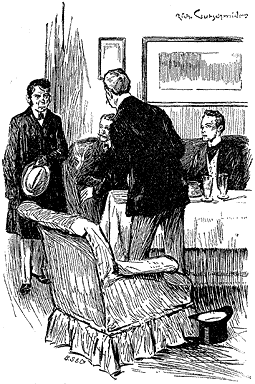
\includegraphics{images/study10-stud-11.png}\end{center}

\noindent \begin{center}\noun{Lestrade stood in the centre of the
room, fumbling nervously with his hat and uncertain what to do.}\end{center}
\end{figure}
He had evidently come with the intention of consulting with Sherlock
Holmes, for on perceiving his colleague he appeared to be embarrassed
and put out. He stood in the centre of the room, fumbling nervously
with his hat and uncertain what to do. {}``This is a most extraordinary
case,'' he said at last\mdsh{---}{}``a most incomprehensible affair.''

{}``Ah, you find it so, Mr.\ Lestrade!'' cried Gregson, triumphantly.
{}``I thought you would come to that conclusion. Have you managed
to find the Secretary, Mr.\ Joseph Stangerson?''

{}``The Secretary, Mr.\ Joseph Stangerson,'' said Lestrade gravely,
{}``was murdered at Halliday's Private Hotel about six o'clock this
morning.''


\chapter*{\raggedright CHAPTER VII. LIGHT IN THE DARKNESS.}

\addcontentsline{toc}{chapter}{CHAPTER VII. LIGHT IN THE DARKNESS.}

\markboth{A STUDY IN SCARLET}{CHAPTER VII}

The intelligence with which Lestrade greeted us was so momentous and
so unexpected, that we were all three fairly dumfoundered. Gregson
sprang out of his chair and upset the remainder of his whiskey and
water. I stared in silence at Sherlock Holmes, whose lips were compressed
and his brows drawn down over his eyes.

{}``Stangerson too!'' he muttered. {}``The plot thickens.''

{}``It was quite thick enough before,'' grumbled Lestrade, taking
a chair. {}``I seem to have dropped into a sort of council of war.''

{}``Are you\mdsh{---}are you sure of this piece of intelligence?''
stammered Gregson.

{}``I have just come from his room,'' said Lestrade. {}``I was
the first to discover what had occurred.''

{}``We have been hearing Gregson's view of the matter,'' Holmes
observed. {}``Would you mind letting us know what you have seen and
done?''

{}``I have no objection,'' Lestrade answered, seating himself. {}``I
freely confess that I was of the opinion that Stangerson was concerned
in the death of Drebber. This fresh development has shown me that
I was completely mistaken. Full of the one idea, I set myself to find
out what had become of the Secretary. They had been seen together
at Euston Station about half-past eight on the evening of the third.
At two in the morning Drebber had been found in the Brixton Road.
The question which confronted me was to find out how Stangerson had
been employed between 8.30 and the time of the crime, and what had
become of him afterwards. I telegraphed to Liverpool, giving a description
of the man, and warning them to keep a watch upon the American boats.
I then set to work calling upon all the hotels and lodging-houses
in the vicinity of Euston. You see, I argued that if Drebber and his
companion had become separated, the natural course for the latter
would be to put up somewhere in the vicinity for the night, and then
to hang about the station again next morning.''

{}``They would be likely to agree on some meeting-place beforehand,''
remarked Holmes.

{}``So it proved. I spent the whole of yesterday evening in making
enquiries entirely without avail. This morning I began very early,
and at eight o'clock I reached Halliday's Private Hotel, in Little
George Street. On my enquiry as to whether a Mr.\ Stangerson was
living there, they at once answered me in the affirmative.

{}```No doubt you are the gentleman whom he was expecting,' they
said.\  `He has been waiting for a gentleman for two days.'

{}```Where is he now?'\ I asked.

{}```He is upstairs in bed. He wished to be called at nine.'

{}```I will go up and see him at once,' I said.

{}``It seemed to me that my sudden appearance might shake his nerves
and lead him to say something unguarded. The Boots volunteered to
show me the room: it was on the second floor, and there was a small
corridor leading up to it. The Boots pointed out the door to me, and
was about to go downstairs again when I saw something that made me
feel sickish, in spite of my twenty years' experience. From under
the door there curled a little red ribbon of blood, which had meandered
across the passage and formed a little pool along the skirting at
the other side. I gave a cry, which brought the Boots back. He nearly
fainted when he saw it. The door was locked on the inside, but we
put our shoulders to it, and knocked it in. The window of the room
was open, and beside the window, all huddled up, lay the body of a
man in his nightdress. He was quite dead, and had been for some time,
for his limbs were rigid and cold. When we turned him over, the Boots
recognized him at once as being the same gentleman who had engaged
the room under the name of Joseph Stangerson. The cause of death was
a deep stab in the left side, which must have penetrated the heart.
And now comes the strangest part of the affair. What do you suppose
was above the murdered man?''

I felt a creeping of the flesh, and a presentiment of coming horror,
even before Sherlock Holmes answered.

{}``The word RACHE, written in letters of blood,'' he said.

{}``That was it,'' said Lestrade, in an awe-struck voice; and we
were all silent for a while.

There was something so methodical and so incomprehensible about the
deeds of this unknown assassin, that it imparted a fresh ghastliness
to his crimes. My nerves, which were steady enough on the field of
battle tingled as I thought of it.

{}``The man was seen,'' continued Lestrade. {}``A milk boy, passing
on his way to the dairy, happened to walk down the lane which leads
from the mews at the back of the hotel. He noticed that a ladder,
which usually lay there, was raised against one of the windows of
the second floor, which was wide open. After passing, he looked back
and saw a man descend the ladder. He came down so quietly and openly
that the boy imagined him to be some carpenter or joiner at work in
the hotel. He took no particular notice of him, beyond thinking in
his own mind that it was early for him to be at work. He has an impression
that the man was tall, had a reddish face, and was dressed in a long,
brownish coat. He must have stayed in the room some little time after
the murder, for we found blood-stained water in the basin, where he
had washed his hands, and marks on the sheets where he had deliberately
wiped his knife.''

I glanced at Holmes on hearing the description of the murderer, which
tallied so exactly with his own. There was, however, no trace of exultation
or satisfaction upon his face.

{}``Did you find nothing in the room which could furnish a clue to
the murderer?''\ he asked.

{}``Nothing. Stangerson had Drebber's purse in his pocket, but it
seems that this was usual, as he did all the paying. There was eighty
odd pounds in it, but nothing had been taken. Whatever the motives
of these extraordinary crimes, robbery is certainly not one of them.
There were no papers or memoranda in the murdered man's pocket, except
a single telegram, dated from Cleveland about a month ago, and containing
the words, `J. H.\ is in Europe.' There was no name appended to this
message.''

{}``And there was nothing else?''\ Holmes asked.

{}``Nothing of any importance. The man's novel, with which he had
read himself to sleep was lying upon the bed, and his pipe was on
a chair beside him. There was a glass of water on the table, and on
the window-sill a small chip ointment box containing a couple of pills.''

Sherlock Holmes sprang from his chair with an exclamation of delight.

{}``The last link,'' he cried, exultantly. {}``My case is complete.''

The two detectives stared at him in amazement.

{}``I have now in my hands,'' my companion said, confidently, {}``all
the threads which have formed such a tangle. There are, of course,
details to be filled in, but I am as certain of all the main facts,
from the time that Drebber parted from Stangerson at the station,
up to the discovery of the body of the latter, as if I had seen them
with my own eyes. I will give you a proof of my knowledge. Could you
lay your hand upon those pills?''

{}``I have them,'' said Lestrade, producing a small white box; {}``I
took them and the purse and the telegram, intending to have them put
in a place of safety at the Police Station. It was the merest chance
my taking these pills, for I am bound to say that I do not attach
any importance to them.''

{}``Give them here,'' said Holmes. {}``Now, Doctor,'' turning
to me, {}``are those ordinary pills?''

They certainly were not. They were of a pearly grey colour, small,
round, and almost transparent against the light. {}``From their lightness
and transparency, I should imagine that they are soluble in water,''
I remarked.

{}``Precisely so,'' answered Holmes. {}``Now would you mind going
down and fetching that poor little devil of a terrier which has been
bad so long, and which the landlady wanted you to put out of its pain
yesterday.''

I went downstairs and carried the dog upstair in my arms. It's laboured
breathing and glazing eye showed that it was not far from its end.
Indeed, its snow-white muzzle proclaimed that it had already exceeded
the usual term of canine existence. I placed it upon a cushion on
the rug.

{}``I will now cut one of these pills in two,'' said Holmes, and
drawing his penknife he suited the action to the word. {}``One half
we return into the box for future purposes. The other half I will
place in this wine glass, in which is a teaspoonful of water. You
perceive that our friend, the Doctor, is right, and that it readily
dissolves.''

{}``This may be very interesting,'' said Lestrade, in the injured
tone of one who suspects that he is being laughed at, {}``I cannot
see, however, what it has to do with the death of Mr.\ Joseph Stangerson.''

{}``Patience, my friend, patience! You will find in time that it
has everything to do with it. I shall now add a little milk to make
the mixture palatable, and on presenting it to the dog we find that
he laps it up readily enough.''

As he spoke he turned the contents of the wine glass into a saucer
and placed it in front of the terrier, who speedily licked it dry.
Sherlock Holmes' earnest demeanour had so far convinced us that we
all sat in silence, watching the animal intently, and expecting some
startling effect. None such appeared, however. %
\begin{figure}[htbp]
\noindent \begin{center}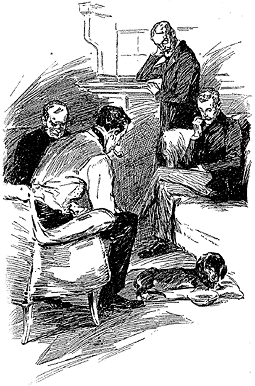
\includegraphics{images/study10-stud-12.png}\end{center}

\noindent \begin{center}\noun{The dog continued to lie stretched
upon the cushion.}\end{center}
\end{figure}
The dog continued to lie stretched upon the cushion, breathing in
a laboured way, but apparently neither the better nor the worse for
its draught.

Holmes had taken out his watch, and as minute followed minute without
result, an expression of the utmost chagrin and disappointment appeared
upon his features. He gnawed his lip, drummed his fingers upon the
table, and showed every other symptom of acute impatience. So great
was his emotion, that I felt sincerely sorry for him, while the two
detectives smiled derisively, by no means displeased at this check
which he had met.

{}``It can't be a coincidence,'' he cried, at last springing from
his chair and pacing wildly up and down the room; {}``it is impossible
that it should be a mere coincidence. The very pills which I suspected
in the case of Drebber are actually found after the death of Stangerson.
And yet they are inert. What can it mean? Surely my whole chain of
reasoning cannot have been false. It is impossible! And yet this wretched
dog is none the worse. Ah, I have it! I have it!'' With a perfect
shriek of delight he rushed to the box, cut the other pill in two,
dissolved it, added milk, and presented it to the terrier. The unfortunate
creature's tongue seemed hardly to have been moistened in it before
it gave a convulsive shiver in every limb, and lay as rigid and lifeless
as if it had been struck by lightning.

Sherlock Holmes drew a long breath, and wiped the perspiration from
his forehead. {}``I should have more faith,'' he said; {}``I ought
to know by this time that when a fact appears to be opposed to a long
train of deductions, it invariably proves to be capable of bearing
some other interpretation. Of the two pills in that box one was of
the most deadly poison, and the other was entirely harmless. I ought
to have known that before ever I saw the box at all.''

This last statement appeared to me to be so startling, that I could
hardly believe that he was in his sober senses. There was the dead
dog, however, to prove that his conjecture had been correct. It seemed
to me that the mists in my own mind were gradually clearing away,
and I began to have a dim, vague perception of the truth.

{}``All this seems strange to you,'' continued Holmes, {}``because
you failed at the beginning of the inquiry to grasp the importance
of the single real clue which was presented to you. I had the good
fortune to seize upon that, and everything which has occurred since
then has served to confirm my original supposition, and, indeed, was
the logical sequence of it. Hence things which have perplexed you
and made the case more obscure, have served to enlighten me and to
strengthen my conclusions. It is a mistake to confound strangeness
with mystery. The most commonplace crime is often the most mysterious
because it presents no new or special features from which deductions
may be drawn. This murder would have been infinitely more difficult
to unravel had the body of the victim been simply found lying in the
roadway without any of those \textit{outr�} and sensational accompaniments
which have rendered it remarkable. These strange details, far from
making the case more difficult, have really had the effect of making
it less so.''

Mr.\ Gregson, who had listened to this address with considerable
impatience, could contain himself no longer. {}``Look here, Mr.\ Sherlock
Holmes,'' he said, {}``we are all ready to acknowledge that you
are a smart man, and that you have your own methods of working. We
want something more than mere theory and preaching now, though. It
is a case of taking the man. I have made my case out, and it seems
I was wrong. Young Charpentier could not have been engaged in this
second affair. Lestrade went after his man, Stangerson, and it appears
that he was wrong too. You have thrown out hints here, and hints there,
and seem to know more than we do, but the time has come when we feel
that we have a right to ask you straight how much you do know of the
business. Can you name the man who did it?''

{}``I cannot help feeling that Gregson is right, sir,'' remarked
Lestrade. {}``We have both tried, and we have both failed. You have
remarked more than once since I have been in the room that you had
all the evidence which you require. Surely you will not withhold it
any longer.''

{}``Any delay in arresting the assassin,'' I observed, {}``might
give him time to perpetrate some fresh atrocity.''

Thus pressed by us all, Holmes showed signs of irresolution. He continued
to walk up and down the room with his head sunk on his chest and his
brows drawn down, as was his habit when lost in thought.

{}``There will be no more murders,'' he said at last, stopping abruptly
and facing us. {}``You can put that consideration out of the question.
You have asked me if I know the name of the assassin. I do. The mere
knowing of his name is a small thing, however, compared with the power
of laying our hands upon him. This I expect very shortly to do. I
have good hopes of managing it through my own arrangements; but it
is a thing which needs delicate handling, for we have a shrewd and
desperate man to deal with, who is supported, as I have had occasion
to prove, by another who is as clever as himself. As long as this
man has no idea that anyone can have a clue there is some chance of
securing him; but if he had the slightest suspicion, he would change
his name, and vanish in an instant among the four million inhabitants
of this great city. Without meaning to hurt either of your feelings,
I am bound to say that I consider these men to be more than a match
for the official force, and that is why I have not asked your assistance.
If I fail I shall, of course, incur all the blame due to this omission;
but that I am prepared for. At present I am ready to promise that
the instant that I can communicate with you without endangering my
own combinations, I shall do so.''

Gregson and Lestrade seemed to be far from satisfied by this assurance,
or by the depreciating allusion to the detective police. The former
had flushed up to the roots of his flaxen hair, while the other's
beady eyes glistened with curiosity and resentment. Neither of them
had time to speak, however, before there was a tap at the door, and
the spokesman of the street Arabs, young Wiggins, introduced his insignificant
and unsavoury person.

{}``Please, sir,'' he said, touching his forelock, {}``I have the
cab downstairs.''

{}``Good boy,'' said Holmes, blandly. {}``Why don't you introduce
this pattern at Scotland Yard?''\ he continued, taking a pair of
steel handcuffs from a drawer. {}``See how beautifully the spring
works. They fasten in an instant.''

{}``The old pattern is good enough,'' remarked Lestrade, {}``if
we can only find the man to put them on.''

{}``Very good, very good,'' said Holmes, smiling. {}``The cabman
may as well help me with my boxes. Just ask him to step up, Wiggins.''

I was surprised to find my companion speaking as though he were about
to set out on a journey, since he had not said anything to me about
it. There was a small portmanteau in the room, and this he pulled
out and began to strap. He was busily engaged at it when the cabman
entered the room.

{}``Just give me a help with this buckle, cabman,'' he said, kneeling
over his task, and never turning his head.

The fellow came forward with a somewhat sullen, defiant air, and put
down his hands to assist. At that instant there was a sharp click,
the jangling of metal, and Sherlock Holmes sprang to his feet again.

{}``Gentlemen,'' he cried, with flashing eyes, {}``let me introduce
you to Mr.\ Jefferson Hope, the murderer of Enoch Drebber and of
Joseph Stangerson.''

The whole thing occurred in a moment\mdsh{---}so quickly that I had
no time to realize it. I have a vivid recollection of that instant,
of Holmes' triumphant expression and the ring of his voice, of the
cabman's dazed, savage face, as he glared at the glittering handcuffs,
which had appeared as if by magic upon his wrists. For a second or
two we might have been a group of statues. Then, with an inarticulate
roar of fury, the prisoner wrenched himself free from Holmes's grasp,
and hurled himself through the window. Woodwork and glass gave way
before him; but before he got quite through, Gregson, Lestrade, and
Holmes sprang upon him like so many staghounds. %
\begin{figure}[htbp]
\noindent \begin{center}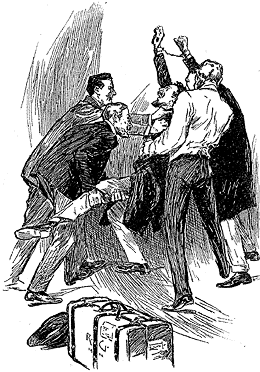
\includegraphics{images/study10-stud-13.png}\end{center}

\noindent \begin{center}\noun{So powerful and so fierce was he,
that the four of us were shaken off again and again.}\end{center}
\end{figure}
He was dragged back into the room, and then commenced a terrific conflict.
So powerful and so fierce was he, that the four of us were shaken
off again and again. He appeared to have the convulsive strength of
a man in an epileptic fit. His face and hands were terribly mangled
by his passage through the glass, but loss of blood had no effect
in diminishing his resistance. It was not until Lestrade succeeded
in getting his hand inside his neckcloth and half-strangling him that
we made him realize that his struggles were of no avail; and even
then we felt no security until we had pinioned his feet as well as
his hands. That done, we rose to our feet breathless and panting.

{}``We have his cab,'' said Sherlock Holmes. {}``It will serve
to take him to Scotland Yard. And now, gentlemen,'' he continued,
with a pleasant smile, {}``we have reached the end of our little
mystery. You are very welcome to put any questions that you like to
me now, and there is no danger that I will refuse to answer them.''


\part*{PART II.\textit{}\protect \\
\textit{\normalsize The Country of the Saints.}}



\addcontentsline{toc}{part}{PART II}

\markboth{A STUDY IN SCARLET}{PART II}


\chapter*{\raggedright CHAPTER I. ON THE GREAT ALKALI PLAIN.}



\addcontentsline{toc}{chapter}{CHAPTER I. ON THE GREAT ALKALI\\
PLAIN.}

\markboth{A STUDY IN SCARLET}{CHAPTER I}

In the central portion of the great North American Continent there
lies an arid and repulsive desert, which for many a long year served
as a barrier against the advance of civilisation. From the Sierra
Nevada to Nebraska, and from the Yellowstone River in the north to
the Colorado upon the south, is a region of desolation and silence.
Nor is Nature always in one mood throughout this grim district. It
comprises snow-capped and lofty mountains, and dark and gloomy valleys.
There are swift-flowing rivers which dash through jagged ca�ons; and
there are enormous plains, which in winter are white with snow, and
in summer are grey with the saline alkali dust. They all preserve,
however, the common characteristics of barrenness, inhospitality,
and misery.

There are no inhabitants of this land of despair. A band of Pawnees
or of Blackfeet may occasionally traverse it in order to reach other
hunting-grounds, but the hardiest of the braves are glad to lose sight
of those awesome plains, and to find themselves once more upon their
prairies. The coyote skulks among the scrub, the buzzard flaps heavily
through the air, and the clumsy grizzly bear lumbers through the dark
ravines, and picks up such sustenance as it can amongst the rocks.
These are the sole dwellers in the wilderness.

In the whole world there can be no more dreary view than that from
the northern slope of the Sierra Blanco. As far as the eye can reach
stretches the great flat plain-land, all dusted over with patches
of alkali, and intersected by clumps of the dwarfish chaparral bushes.
On the extreme verge of the horizon lie a long chain of mountain peaks,
with their rugged summits flecked with snow. In this great stretch
of country there is no sign of life, nor of anything appertaining
to life. There is no bird in the steel-blue heaven, no movement upon
the dull, grey earth\mdsh{---}above all, there is absolute silence.
Listen as one may, there is no shadow of a sound in all that mighty
wilderness; nothing but silence\mdsh{---}complete and heart-subduing
silence.

It has been said there is nothing appertaining to life upon the broad
plain. That is hardly true. Looking down from the Sierra Blanco, one
sees a pathway traced out across the desert, which winds away and
is lost in the extreme distance. It is rutted with wheels and trodden
down by the feet of many adventurers. Here and there there are scattered
white objects which glisten in the sun, and stand out against the
dull deposit of alkali. Approach, and examine them! They are bones:
some large and coarse, others smaller and more delicate. The former
have belonged to oxen, and the latter to men. For fifteen hundred
miles one may trace this ghastly caravan route by these scattered
remains of those who had fallen by the wayside.

Looking down on this very scene, there stood upon the fourth of May,
eighteen hundred and forty-seven, a solitary traveller. His appearance
was such that he might have been the very genius or demon of the region.
An observer would have found it difficult to say whether he was nearer
to forty or to sixty. His face was lean and haggard, and the brown
parchment-like skin was drawn tightly over the projecting bones; his
long, brown hair and beard were all flecked and dashed with white;
his eyes were sunken in his head, and burned with an unnatural lustre;
while the hand which grasped his rifle was hardly more fleshy than
that of a skeleton. As he stood, he leaned upon his weapon for support,
and yet his tall figure and the massive framework of his bones suggested
a wiry and vigorous constitution. His gaunt face, however, and his
clothes, which hung so baggily over his shrivelled limbs, proclaimed
what it was that gave him that senile and decrepit appearance. The
man was dying\mdsh{---}dying from hunger and from thirst.

He had toiled painfully down the ravine, and on to this little elevation,
in the vain hope of seeing some signs of water. Now the great salt
plain stretched before his eyes, and the distant belt of savage mountains,
without a sign anywhere of plant or tree, which might indicate the
presence of moisture. In all that broad landscape there was no gleam
of hope. North, and east, and west he looked with wild questioning
eyes, and then he realised that his wanderings had come to an end,
and that there, on that barren crag, he was about to die. {}``Why
not here, as well as in a feather bed, twenty years hence,'' he muttered,
as he seated himself in the shelter of a boulder.

Before sitting down, he had deposited upon the ground his useless
rifle, and also a large bundle tied up in a grey shawl, which he had
carried slung over his right shoulder. It appeared to be somewhat
too heavy for his strength, for in lowering it, it came down on the
ground with some little violence. Instantly there broke from the grey
parcel a little moaning cry, and from it there protruded a small,
scared face, with very bright brown eyes, and two little speckled,
dimpled fists.

{}``You've hurt me!'' said a childish voice reproachfully.

{}``Have I though,'' the man answered penitently, {}``I didn't
go for to do it.'' As he spoke he unwrapped the grey shawl and extricated
a pretty little girl of about five years of age, whose dainty shoes
and smart pink frock with its little linen apron all bespoke a mother's
care. The child was pale and wan, but her healthy arms and legs showed
that she had suffered less than her companion.

{}``How is it now?''\ he answered anxiously, for she was still
rubbing the towsy golden curls which covered the back of her head.

{}``Kiss it and make it well,'' she said, with perfect gravity,
shoving the injured part up to him. {}``That's what mother used to
do. Where's mother?''

{}``Mother's gone. I guess you'll see her before long.''

{}``Gone, eh!''\ said the little girl. {}``Funny, she didn't say
good-bye; she 'most always did if she was just goin' over to Auntie's
for tea, and now she's been away three days. Say, it's awful dry,
ain't it? Ain't there no water, nor nothing to eat?''

{}``No, there ain't nothing, dearie. You'll just need to be patient
awhile, and then you'll be all right. Put your head up agin me like
that, and then you'll feel bullier. It ain't easy to talk when your
lips is like leather, but I guess I'd best let you know how the cards
lie. What's that you've got?''

{}``Pretty things!\ fine things!''\ cried the little girl enthusiastically,
holding up two glittering fragments of mica. {}``When we goes back
to home I'll give them to brother Bob.''

{}``You'll see prettier things than them soon,'' said the man confidently.
{}``You just wait a bit. I was going to tell you though\mdsh{---}you
remember when we left the river?''

{}``Oh, yes.''

{}``Well, we reckoned we'd strike another river soon, d'ye see. But
there was somethin' wrong; compasses, or map, or somethin', and it
didn't turn up. Water ran out. Just except a little drop for the likes
of you and\mdsh{---}and\mbox{---}''

{}``And you couldn't wash yourself,'' interrupted his companion
gravely, staring up at his grimy visage.

{}``No, nor drink. And Mr.\ Bender, he was the fust to go, and then
Indian Pete, and then Mrs.\ McGregor, and then Johnny Hones, and
then, dearie, your mother.''

{}``Then mother's a deader too,'' cried the little girl dropping
her face in her pinafore and sobbing bitterly.

{}``Yes, they all went except you and me. Then I thought there was
some chance of water in this direction, so I heaved you over my shoulder
and we tramped it together. It don't seem as though we've improved
matters. There's an almighty small chance for us now!''

{}``Do you mean that we are going to die too?'' asked the child,
checking her sobs, and raising her tear-stained face.

{}``I guess that's about the size of it.''

{}``Why didn't you say so before?'' she said, laughing gleefully.
{}``You gave me such a fright. Why, of course, now as long as we
die we'll be with mother again.''

{}``Yes, you will, dearie.''

{}``And you too. I'll tell her how awful good you've been. I'll bet
she meets us at the door of Heaven with a big pitcher of water, and
a lot of buckwheat cakes, hot, and toasted on both sides, like Bob
and me was fond of. How long will it be first?''

{}``I don't know\mdsh{---}not very long.'' The man's eyes were
fixed upon the northern horizon. In the blue vault of the heaven there
had appeared three little specks which increased in size every moment,
so rapidly did they approach. They speedily resolved themselves into
three large brown birds, which circled over the heads of the two wanderers,
and then settled upon some rocks which overlooked them. They were
buzzards, the vultures of the west, whose coming is the forerunner
of death.

{}``Cocks and hens,'' cried the little girl gleefully, pointing
at their ill-omened forms, and clapping her hands to make them rise.
{}``Say, did God make this country?''

{}``In course He did,'' said her companion, rather startled by this
unexpected question.

{}``He made the country down in Illinois, and He made the Missouri,''
the little girl continued. {}``I guess somebody else made the country
in these parts. It's not nearly so well done. They forgot the water
and the trees.''

{}``What would ye think of offering up prayer?'' the man asked diffidently.

{}``It ain't night yet,'' she answered.

{}``It don't matter. It ain't quite regular, but He won't mind that,
you bet. You say over them ones that you used to say every night in
the waggon when we was on the Plains.''

{}``Why don't you say some yourself?''\ the child asked, with wondering
eyes.

{}``I disremember them,'' he answered. {}``I hain't said none since
I was half the height o' that gun. I guess it's never too late. You
say them out, and I'll stand by and come in on the choruses.''

%
\begin{figure}[htbp]
\noindent \begin{center}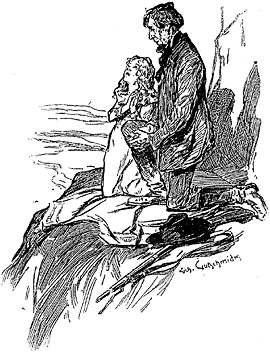
\includegraphics{images/study10-stud-14.png}\end{center}

\noindent \begin{center}\noun{{}``You've got to put your hands
up like this. It makes you feel kind o' good.''}\end{center}
\end{figure}
{}``Then you'll need to kneel down, and me too,'' she said, laying
the shawl out for that purpose. {}``You've got to put your hands
up like this. It makes you feel kind o' good.''

It was a strange sight had there been anything but the buzzards to
see it. Side by side on the narrow shawl knelt the two wanderers,
the little prattling child and the reckless, hardened adventurer.
Her chubby face, and his haggard, angular visage were both turned
up to the cloudless heaven in heartfelt entreaty to that dread being
with whom they were face to face, while the two voices\mdsh{---}the
one thin and clear, the other deep and harsh\mdsh{---}united in the
entreaty for mercy and forgiveness. The prayer finished, they resumed
their seat in the shadow of the boulder until the child fell asleep,
nestling upon the broad breast of her protector. He watched over her
slumber for some time, but Nature proved to be too strong for him.
For three days and three nights he had allowed himself neither rest
nor repose. Slowly the eyelids drooped over the tired eyes, and the
head sunk lower and lower upon the breast, until the man's grizzled
beard was mixed with the gold tresses of his companion, and both slept
the same deep and dreamless slumber.

Had the wanderer remained awake for another half hour a strange sight
would have met his eyes. Far away on the extreme verge of the alkali
plain there rose up a little spray of dust, very slight at first,
and hardly to be distinguished from the mists of the distance, but
gradually growing higher and broader until it formed a solid, well-defined
cloud. This cloud continued to increase in size until it became evident
that it could only be raised by a great multitude of moving creatures.
In more fertile spots the observer would have come to the conclusion
that one of those great herds of bisons which graze upon the prairie
land was approaching him. This was obviously impossible in these arid
wilds. As the whirl of dust drew nearer to the solitary bluff upon
which the two castaways were reposing, the canvas-covered tilts of
waggons and the figures of armed horsemen began to show up through
the haze, and the apparition revealed itself as being a great caravan
upon its journey for the West. But what a caravan! When the head of
it had reached the base of the mountains, the rear was not yet visible
on the horizon. Right across the enormous plain stretched the straggling
array, waggons and carts, men on horseback, and men on foot. Innumerable
women who staggered along under burdens, and children who toddled
beside the waggons or peeped out from under the white coverings. This
was evidently no ordinary party of immigrants, but rather some nomad
people who had been compelled from stress of circumstances to seek
themselves a new country. There rose through the clear air a confused
clattering and rumbling from this great mass of humanity, with the
creaking of wheels and the neighing of horses. Loud as it was, it
was not sufficient to rouse the two tired wayfarers above them.

At the head of the column there rode a score or more of grave ironfaced
men, clad in sombre homespun garments and armed with rifles. On reaching
the base of the bluff they halted, and held a short council among
themselves.

{}``The wells are to the right, my brothers,'' said one, a hard-lipped,
clean-shaven man with grizzly hair.

{}``To the right of the Sierra Blanco\mdsh{---}so we shall reach
the Rio Grande,'' said another.

{}``Fear not for water,'' cried a third. {}``He who could draw
it from the rocks will not now abandon His own chosen people.''

{}``Amen!\ Amen!''\ responded the whole party.

They were about to resume their journey when one of the youngest and
keenest-eyed uttered an exclamation and pointed up at the rugged crag
above them. From its summit there fluttered a little wisp of pink,
showing up hard and bright against the grey rocks behind. At the sight
there was a general reining up of horses and unslinging of guns, while
fresh horsemen came galloping up to reinforce the vanguard. The word
`Redskins' was on every lip.

{}``There can't be any number of Injuns here,'' said the elderly
man who appeared to be in command. {}``We have passed the Pawnees,
and there are no other tribes until we cross the great mountains.''

{}``Shall I go forward and see, Brother Stangerson,'' asked one
of the band.

{}``And I,'' {}``and I,'' cried a dozen voices.

{}``Leave your horses below and we will await you here,'' the Elder
answered. In a moment the young fellows had dismounted, fastened their
horses, and were ascending the precipitous slope which led up to the
object which had excited their curiosity. They advanced rapidly and
noiselessly, with the confidence and dexterity of practised scouts.
The watchers from the plain below could see them flit from rock to
rock until their figures stood out against the skyline. The young
man who had first given the alarm was leading them. Suddenly his followers
saw him throw up his hands, as though overcome with astonishment,
and on joining him they were affected in the same way by the sight
which met their eyes.

On the little plateau which crowned the barren hill there stood a
single giant boulder, and against this boulder there lay a tall man,
long-bearded and hard-featured, but of an excessive thinness. His
placid face and regular breathing showed that he was fast asleep.
Beside him lay a little child, with her round white arms encircling
his brown sinewy neck, and her golden haired head resting upon the
breast of his velveteen tunic. Her rosy lips were parted, showing
the regular line of snow-white teeth within, and a playful smile played
over her infantile features. Her plump little white legs terminating
in white socks and neat shoes with shining buckles, offered a strange
contrast to the long shrivelled members of her companion. On the ledge
of rock above this strange couple there stood three solemn buzzards,
who, at the sight of the new comers uttered raucous screams of disappointment
and flapped sullenly away.

The cries of the foul birds awoke the two sleepers who stared about
them in bewilderment. The man staggered to his feet and looked down
upon the plain which had been so desolate when sleep had overtaken
him, and which was now traversed by this enormous body of men and
of beasts. His face assumed an expression of incredulity as he gazed,
and he passed his boney hand over his eyes. {}``This is what they
call delirium, I guess,'' he muttered. The child stood beside him,
holding on to the skirt of his coat, and said nothing but looked all
round her with the wondering questioning gaze of childhood.

%
\begin{figure}[htbp]
\noindent \begin{center}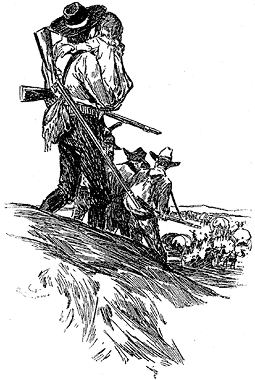
\includegraphics{images/study10-stud-15.png}\end{center}

\noindent \begin{center}\noun{One of them seized the little girl,
and hoisted her upon his shoulder.}\end{center}
\end{figure}
The rescuing party were speedily able to convince the two castaways
that their appearance was no delusion. One of them seized the little
girl, and hoisted her upon his shoulder, while two others supported
her gaunt companion, and assisted him towards the waggons.

{}``My name is John Ferrier,'' the wanderer explained; {}``me and
that little un are all that's left o' twenty-one people. The rest
is all dead o' thirst and hunger away down in the south.''

{}``Is she your child?'' asked someone.

{}``I guess she is now,'' the other cried, defiantly; {}``she's
mine 'cause I saved her. No man will take her from me. She's Lucy
Ferrier from this day on. Who are you, though?'' he continued, glancing
with curiosity at his stalwart, sunburned rescuers; {}``there seems
to be a powerful lot of ye.''

{}``Nigh upon ten thousand,'' said one of the young men; {}``we
are the persecuted children of God\mdsh{---}the chosen of the Angel
Merona.''

{}``I never heard tell on him,'' said the wanderer. {}``He appears
to have chosen a fair crowd of ye.''

{}``Do not jest at that which is sacred,'' said the other sternly.
{}``We are of those who believe in those sacred writings, drawn in
Egyptian letters on plates of beaten gold, which were handed unto
the holy Joseph Smith at Palmyra. We have come from Nauvoo, in the
State of Illinois, where we had founded our temple. We have come to
seek a refuge from the violent man and from the godless, even though
it be the heart of the desert.''

The name of Nauvoo evidently recalled recollections to John Ferrier.
{}``I see,'' he said, {}``you are the Mormons.''

{}``We are the Mormons,'' answered his companions with one voice.

{}``And where are you going?''

{}``We do not know. The hand of God is leading us under the person
of our Prophet. You must come before him. He shall say what is to
be done with you.''

They had reached the base of the hill by this time, and were surrounded
by crowds of the pilgrims\mdsh{---}pale-faced meek-looking women,
strong laughing children, and anxious earnest-eyed men. Many were
the cries of astonishment and of commiseration which arose from them
when they perceived the youth of one of the strangers and the destitution
of the other. Their escort did not halt, however, but pushed on, followed
by a great crowd of Mormons, until they reached a waggon, which was
conspicuous for its great size and for the gaudiness and smartness
of its appearance. Six horses were yoked to it, whereas the others
were furnished with two, or, at most, four apiece. Beside the driver
there sat a man who could not have been more than thirty years of
age, but whose massive head and resolute expression marked him as
a leader. He was reading a brown-backed volume, but as the crowd approached
he laid it aside, and listened attentively to an account of the episode.
Then he turned to the two castaways.

{}``If we take you with us,'' he said, in solemn words, {}``it
can only be as believers in our own creed. We shall have no wolves
in our fold. Better far that your bones should bleach in this wilderness
than that you should prove to be that little speck of decay which
in time corrupts the whole fruit. Will you come with us on these terms?''

{}``Guess I'll come with you on any terms,'' said Ferrier, with
such emphasis that the grave Elders could not restrain a smile. The
leader alone retained his stern, impressive expression.

{}``Take him, Brother Stangerson,'' he said, {}``give him food
and drink, and the child likewise. Let it be your task also to teach
him our holy creed. We have delayed long enough. Forward! On, on to
Zion!''

{}``On, on to Zion!''\ cried the crowd of Mormons, and the words
rippled down the long caravan, passing from mouth to mouth until they
died away in a dull murmur in the far distance. With a cracking of
whips and a creaking of wheels the great waggons got into motion,
and soon the whole caravan was winding along once more. The Elder
to whose care the two waifs had been committed, led them to his waggon,
where a meal was already awaiting them.

{}``You shall remain here,'' he said. {}``In a few days you will
have recovered from your fatigues. In the meantime, remember that
now and for ever you are of our religion. Brigham Young has said it,
and he has spoken with the voice of Joseph Smith, which is the voice
of God.''


\chapter*{\raggedright CHAPTER II. THE FLOWER OF UTAH.}

\addcontentsline{toc}{chapter}{CHAPTER II. THE FLOWER OF UTAH.}

\markboth{A STUDY IN SCARLET}{CHAPTER II}

This is not the place to commemorate the trials and privations endured
by the immigrant Mormons before they came to their final haven. From
the shores of the Mississippi to the western slopes of the Rocky Mountains
they had struggled on with a constancy almost unparalleled in history.
The savage man, and the savage beast, hunger, thirst, fatigue, and
disease\mdsh{---}every impediment which Nature could place in the
way, had all been overcome with Anglo-Saxon tenacity. Yet the long
journey and the accumulated terrors had shaken the hearts of the stoutest
among them. There was not one who did not sink upon his knees in heartfelt
prayer when they saw the broad valley of Utah bathed in the sunlight
beneath them, and learned from the lips of their leader that this
was the promised land, and that these virgin acres were to be theirs
for evermore.

Young speedily proved himself to be a skilful administrator as well
as a resolute chief. Maps were drawn and charts prepared, in which
the future city was sketched out. All around farms were apportioned
and allotted in proportion to the standing of each individual. The
tradesman was put to his trade and the artisan to his calling. In
the town streets and squares sprang up, as if by magic. In the country
there was draining and hedging, planting and clearing, until the next
summer saw the whole country golden with the wheat crop. Everything
prospered in the strange settlement. Above all, the great temple which
they had erected in the centre of the city grew ever taller and larger.
From the first blush of dawn until the closing of the twilight, the
clatter of the hammer and the rasp of the saw was never absent from
the monument which the immigrants erected to Him who had led them
safe through many dangers.

The two castaways, John Ferrier and the little girl who had shared
his fortunes and had been adopted as his daughter, accompanied the
Mormons to the end of their great pilgrimage. Little Lucy Ferrier
was borne along pleasantly enough in Elder Stangerson's waggon, a
retreat which she shared with the Mormon's three wives and with his
son, a headstrong forward boy of twelve. Having rallied, with the
elasticity of childhood, from the shock caused by her mother's death,
she soon became a pet with the women, and reconciled herself to this
new life in her moving canvas-covered home. In the meantime Ferrier
having recovered from his privations, distinguished himself as a useful
guide and an indefatigable hunter. So rapidly did he gain the esteem
of his new companions, that when they reached the end of their wanderings,
it was unanimously agreed that he should be provided with as large
and as fertile a tract of land as any of the settlers, with the exception
of Young himself, and of Stangerson, Kemball, Johnston, and Drebber,
who were the four principal Elders.

On the farm thus acquired John Ferrier built himself a substantial
log-house, which received so many additions in succeeding years that
it grew into a roomy villa. He was a man of a practical turn of mind,
keen in his dealings and skilful with his hands. His iron constitution
enabled him to work morning and evening at improving and tilling his
lands. Hence it came about that his farm and all that belonged to
him prospered exceedingly. In three years he was better off than his
neighbours, in six he was well-to-do, in nine he was rich, and in
twelve there were not half a dozen men in the whole of Salt Lake City
who could compare with him. From the great inland sea to the distant
Wahsatch Mountains there was no name better known than that of John
Ferrier.

There was one way and only one in which he offended the susceptibilities
of his co-religionists. No argument or persuasion could ever induce
him to set up a female establishment after the manner of his companions.
He never gave reasons for this persistent refusal, but contented himself
by resolutely and inflexibly adhering to his determination. There
were some who accused him of lukewarmness in his adopted religion,
and others who put it down to greed of wealth and reluctance to incur
expense. Others, again, spoke of some early love affair, and of a
fair-haired girl who had pined away on the shores of the Atlantic.
Whatever the reason, Ferrier remained strictly celibate. In every
other respect he conformed to the religion of the young settlement,
and gained the name of being an orthodox and straight-walking man.

Lucy Ferrier grew up within the log-house, and assisted her adopted
father in all his undertakings. The keen air of the mountains and
the balsamic odour of the pine trees took the place of nurse and mother
to the young girl. As year succeeded to year she grew taller and stronger,
her cheek more rudy, and her step more elastic. Many a wayfarer upon
the high road which ran by Ferrier's farm felt long-forgotten thoughts
revive in their mind as they watched her lithe girlish figure tripping
through the wheatfields, or met her mounted upon her father's mustang,
and managing it with all the ease and grace of a true child of the
West. So the bud blossomed into a flower, and the year which saw her
father the richest of the farmers left her as fair a specimen of American
girlhood as could be found in the whole Pacific slope.

It was not the father, however, who first discovered that the child
had developed into the woman. It seldom is in such cases. That mysterious
change is too subtle and too gradual to be measured by dates. Least
of all does the maiden herself know it until the tone of a voice or
the touch of a hand sets her heart thrilling within her, and she learns,
with a mixture of pride and of fear, that a new and a larger nature
has awoken within her. There are few who cannot recall that day and
remember the one little incident which heralded the dawn of a new
life. In the case of Lucy Ferrier the occasion was serious enough
in itself, apart from its future influence on her destiny and that
of many besides.

It was a warm June morning, and the Latter Day Saints were as busy
as the bees whose hive they have chosen for their emblem. In the fields
and in the streets rose the same hum of human industry. Down the dusty
high roads defiled long streams of heavily-laden mules, all heading
to the west, for the gold fever had broken out in California, and
the Overland Route lay through the City of the Elect. There, too,
were droves of sheep and bullocks coming in from the outlying pasture
lands, and trains of tired immigrants, men and horses equally weary
of their interminable journey. Through all this motley assemblage,
threading her way with the skill of an accomplished rider, there galloped
Lucy Ferrier, her fair face flushed with the exercise and her long
chestnut hair floating out behind her. She had a commission from her
father in the City, and was dashing in as she had done many a time
before, with all the fearlessness of youth, thinking only of her task
and how it was to be performed. The travel-stained adventurers gazed
after her in astonishment, and even the unemotional Indians, journeying
in with their pelties, relaxed their accustomed stoicism as they marvelled
at the beauty of the pale-faced maiden.

She had reached the outskirts of the city when she found the road
blocked by a great drove of cattle, driven by a half-dozen wild-looking
herdsmen from the plains. In her impatience she endeavoured to pass
this obstacle by pushing her horse into what appeared to be a gap.
Scarcely had she got fairly into it, however, before the beasts closed
in behind her, and she found herself completely imbedded in the moving
stream of fierce-eyed, long-horned bullocks. Accustomed as she was
to deal with cattle, she was not alarmed at her situation, but took
advantage of every opportunity to urge her horse on in the hopes of
pushing her way through the cavalcade. Unfortunately the horns of
one of the creatures, either by accident or design, came in violent
contact with the flank of the mustang, and excited it to madness.
In an instant it reared up upon its hind legs with a snort of rage,
and pranced and tossed in a way that would have unseated any but a
most skilful rider. The situation was full of peril. Every plunge
of the excited horse brought it against the horns again, and goaded
it to fresh madness. It was all that the girl could do to keep herself
in the saddle, yet a slip would mean a terrible death under the hoofs
of the unwieldy and terrified animals. Unaccustomed to sudden emergencies,
her head began to swim, and her grip upon the bridle to relax. Choked
by the rising cloud of dust and by the steam from the struggling creatures,
she might have abandoned her efforts in despair, but for a kindly
voice at her elbow which assured her of assistance. %
\begin{figure}[htbp]
\noindent \begin{center}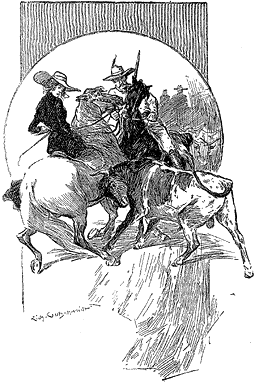
\includegraphics{images/study10-stud-16.png}\end{center}

\noindent \begin{center}\noun{A sinewy brown hand caught the frightened
horse by the curb.}\end{center}
\end{figure}
At the same moment a sinewy brown hand caught the frightened horse
by the curb, and forcing a way through the drove, soon brought her
to the outskirts.

{}``You're not hurt, I hope, miss,'' said her preserver, respectfully.

She looked up at his dark, fierce face, and laughed saucily. {}``I'm
awful frightened,'' she said, naively; {}``whoever would have thought
that Poncho would have been so scared by a lot of cows?''

{}``Thank God you kept your seat,'' the other said earnestly. He
was a tall, savage-looking young fellow, mounted on a powerful roan
horse, and clad in the rough dress of a hunter, with a long rifle
slung over his shoulders. {}``I guess you are the daughter of John
Ferrier,'' he remarked, {}``I saw you ride down from his house.
When you see him, ask him if he remembers the Jefferson Hopes of St.\ Louis.
If he's the same Ferrier, my father and he were pretty thick.''

{}``Hadn't you better come and ask yourself?''\ she asked, demurely.

The young fellow seemed pleased at the suggestion, and his dark eyes
sparkled with pleasure. {}``I'll do so,'' he said, {}``we've been
in the mountains for two months, and are not over and above in visiting
condition. He must take us as he finds us.''

{}``He has a good deal to thank you for, and so have I,'' she answered,
{}``he's awful fond of me. If those cows had jumped on me he'd have
never got over it.''

{}``Neither would I,'' said her companion.

{}``You! Well, I don't see that it would make much matter to you,
anyhow. You ain't even a friend of ours.''

The young hunter's dark face grew so gloomy over this remark that
Lucy Ferrier laughed aloud.

{}``There, I didn't mean that,'' she said; {}``of course, you are
a friend now. You must come and see us. Now I must push along, or
father won't trust me with his business any more. Good-bye!''

{}``Good-bye,'' he answered, raising his broad sombrero, and bending
over her little hand. She wheeled her mustang round, gave it a cut
with her riding-whip, and darted away down the broad road in a rolling
cloud of dust.

Young Jefferson Hope rode on with his companions, gloomy and taciturn.
He and they had been among the Nevada Mountains prospecting for silver,
and were returning to Salt Lake City in the hope of raising capital
enough to work some lodes which they had discovered. He had been as
keen as any of them upon the business until this sudden incident had
drawn his thoughts into another channel. The sight of the fair young
girl, as frank and wholesome as the Sierra breezes, had stirred his
volcanic, untamed heart to its very depths. When she had vanished
from his sight, he realized that a crisis had come in his life, and
that neither silver speculations nor any other questions could ever
be of such importance to him as this new and all-absorbing one. The
love which had sprung up in his heart was not the sudden, changeable
fancy of a boy, but rather the wild, fierce passion of a man of strong
will and imperious temper. He had been accustomed to succeed in all
that he undertook. He swore in his heart that he would not fail in
this if human effort and human perseverance could render him successful.

He called on John Ferrier that night, and many times again, until
his face was a familiar one at the farm-house. John, cooped up in
the valley, and absorbed in his work, had had little chance of learning
the news of the outside world during the last twelve years. All this
Jefferson Hope was able to tell him, and in a style which interested
Lucy as well as her father. He had been a pioneer in California, and
could narrate many a strange tale of fortunes made and fortunes lost
in those wild, halcyon days. He had been a scout too, and a trapper,
a silver explorer, and a ranchman. Wherever stirring adventures were
to be had, Jefferson Hope had been there in search of them. He soon
became a favourite with the old farmer, who spoke eloquently of his
virtues. On such occasions, Lucy was silent, but her blushing cheek
and her bright, happy eyes, showed only too clearly that her young
heart was no longer her own. Her honest father may not have observed
these symptoms, but they were assuredly not thrown away upon the man
who had won her affections.

It was a summer evening when he came galloping down the road and pulled
up at the gate. She was at the doorway, and came down to meet him.
He threw the bridle over the fence and strode up the pathway.

{}``I am off, Lucy,'' he said, taking her two hands in his, and
gazing tenderly down into her face; {}``I won't ask you to come with
me now, but will you be ready to come when I am here again?''

{}``And when will that be?'' she asked, blushing and laughing.

{}``A couple of months at the outside. I will come and claim you
then, my darling. There's no one who can stand between us.''

{}``And how about father?'' she asked.

{}``He has given his consent, provided we get these mines working
all right. I have no fear on that head.''

{}``Oh, well; of course, if you and father have arranged it all,
there's no more to be said,'' she whispered, with her cheek against
his broad breast.

%
\begin{figure}[htbp]
\noindent \begin{center}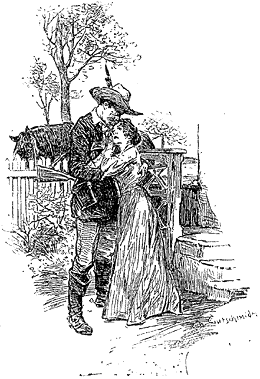
\includegraphics{images/study10-stud-17.png}\end{center}

\noindent \begin{center}\noun{{}``The longer I stay, the harder
it will be to go.''}\end{center}
\end{figure}
{}``Thank God!''\ he said, hoarsely, stooping and kissing her.
{}``It is settled, then. The longer I stay, the harder it will be
to go. They are waiting for me at the ca�on. Good-bye, my own darling\mdsh{---}good-bye.
In two months you shall see me.''

He tore himself from her as he spoke, and, flinging himself upon his
horse, galloped furiously away, never even looking round, as though
afraid that his resolution might fail him if he took one glance at
what he was leaving. She stood at the gate, gazing after him until
he vanished from her sight. Then she walked back into the house, the
happiest girl in all Utah.


\chapter*{\raggedright CHAPTER III. JOHN FERRIER TALKS WITH THE PROPHET.}

\addcontentsline{toc}{chapter}{CHAPTER III. JOHN FERRIER TALKS\\
WITH THE PROPHET.}

\markboth{A STUDY IN SCARLET}{CHAPTER III}

Three weeks had passed since Jefferson Hope and his comrades had departed
from Salt Lake City. John Ferrier's heart was sore within him when
he thought of the young man's return, and of the impending loss of
his adopted child. Yet her bright and happy face reconciled him to
the arrangement more than any argument could have done. He had always
determined, deep down in his resolute heart, that nothing would ever
induce him to allow his daughter to wed a Mormon. Such a marriage
he regarded as no marriage at all, but as a shame and a disgrace.
Whatever he might think of the Mormon doctrines, upon that one point
he was inflexible. He had to seal his mouth on the subject, however,
for to express an unorthodox opinion was a dangerous matter in those
days in the Land of the Saints.

Yes, a dangerous matter\mdsh{---}so dangerous that even the most
saintly dared only whisper their religious opinions with bated breath,
lest something which fell from their lips might be misconstrued, and
bring down a swift retribution upon them. The victims of persecution
had now turned persecutors on their own account, and persecutors of
the most terrible description. Not the Inquisition of Seville, nor
the German Vehmgericht, nor the Secret Societies of Italy, were ever
able to put a more formidable machinery in motion than that which
cast a cloud over the State of Utah.

Its invisibility, and the mystery which was attached to it, made this
organization doubly terrible. It appeared to be omniscient and omnipotent,
and yet was neither seen nor heard. The man who held out against the
Church vanished away, and none knew whither he had gone or what had
befallen him. His wife and his children awaited him at home, but no
father ever returned to tell them how he had fared at the hands of
his secret judges. A rash word or a hasty act was followed by annihilation,
and yet none knew what the nature might be of this terrible power
which was suspended over them. No wonder that men went about in fear
and trembling, and that even in the heart of the wilderness they dared
not whisper the doubts which oppressed them.

At first this vague and terrible power was exercised only upon the
recalcitrants who, having embraced the Mormon faith, wished afterwards
to pervert or to abandon it. Soon, however, it took a wider range.
The supply of adult women was running short, and polygamy without
a female population on which to draw was a barren doctrine indeed.
Strange rumours began to be bandied about\mdsh{---}rumours of murdered
immigrants and rifled camps in regions where Indians had never been
seen. Fresh women appeared in the harems of the Elders\mdsh{---}women
who pined and wept, and bore upon their faces the traces of an unextinguishable
horror. Belated wanderers upon the mountains spoke of gangs of armed
men, masked, stealthy, and noiseless, who flitted by them in the darkness.
These tales and rumours took substance and shape, and were corroborated
and re-corroborated, until they resolved themselves into a definite
name. To this day, in the lonely ranches of the West, the name of
the Danite Band, or the Avenging Angels, is a sinister and an ill-omened
one.

Fuller knowledge of the organization which produced such terrible
results served to increase rather than to lessen the horror which
it inspired in the minds of men. None knew who belonged to this ruthless
society. The names of the participators in the deeds of blood and
violence done under the name of religion were kept profoundly secret.
The very friend to whom you communicated your misgivings as to the
Prophet and his mission, might be one of those who would come forth
at night with fire and sword to exact a terrible reparation. Hence
every man feared his neighbour, and none spoke of the things which
were nearest his heart.

One fine morning, John Ferrier was about to set out to his wheatfields,
when he heard the click of the latch, and, looking through the window,
saw a stout, sandy-haired, middle-aged man coming up the pathway.
His heart leapt to his mouth, for this was none other than the great
Brigham Young himself. Full of trepidation\mdsh{---}for he knew that
such a visit boded him little good\mdsh{---}Ferrier ran to the door
to greet the Mormon chief. The latter, however, received his salutations
coldly, and followed him with a stern face into the sitting-room.

{}``Brother Ferrier,'' he said, taking a seat, and eyeing the farmer
keenly from under his light-coloured eyelashes, {}``the true believers
have been good friends to you. We picked you up when you were starving
in the desert, we shared our food with you, led you safe to the Chosen
Valley, gave you a goodly share of land, and allowed you to wax rich
under our protection. Is not this so?''

{}``It is so,'' answered John Ferrier.

{}``In return for all this we asked but one condition: that was,
that you should embrace the true faith, and conform in every way to
its usages. This you promised to do, and this, if common report says
truly, you have neglected.''

{}``And how have I neglected it?'' asked Ferrier, throwing out his
hands in expostulation. {}``Have I not given to the common fund?
Have I not attended at the Temple? Have I not\mbox{---}?''

{}``Where are your wives?'' asked Young, looking round him. {}``Call
them in, that I may greet them.''

{}``It is true that I have not married,'' Ferrier answered. {}``But
women were few, and there were many who had better claims than I.\ 
I was not a lonely man: I had my daughter to attend to my wants.''

{}``It is of that daughter that I would speak to you,'' said the
leader of the Mormons. {}``She has grown to be the flower of Utah,
and has found favour in the eyes of many who are high in the land.''

John Ferrier groaned internally.

{}``There are stories of her which I would fain disbelieve\mdsh{---}stories
that she is sealed to some Gentile. This must be the gossip of idle
tongues. What is the thirteenth rule in the code of the sainted Joseph
Smith? `Let every maiden of the true faith marry one of the elect;
for if she wed a Gentile, she commits a grievous sin.' This being
so, it is impossible that you, who profess the holy creed, should
suffer your daughter to violate it.''

John Ferrier made no answer, but he played nervously with his riding-whip.

{}``Upon this one point your whole faith shall be tested\mdsh{---}so
it has been decided in the Sacred Council of Four. The girl is young,
and we would not have her wed grey hairs, neither would we deprive
her of all choice. We Elders have many heifers,%
\footnote{Heber C. Kemball, in one of his sermons, alludes to his hundred wives
under this endearing epithet.%
} but our children must also be provided. Stangerson has a son, and
Drebber has a son, and either of them would gladly welcome your daughter
to their house. Let her choose between them. They are young and rich,
and of the true faith. What say you to that?''

Ferrier remained silent for some little time with his brows knitted.

{}``You will give us time,'' he said at last. {}``My daughter is
very young\mdsh{---}she is scarce of an age to marry.''

{}``She shall have a month to choose,'' said Young, rising from
his seat. {}``At the end of that time she shall give her answer.''

%
\begin{figure}[htbp]
\noindent \begin{center}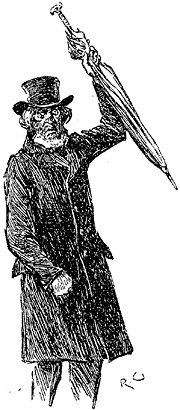
\includegraphics[%
  height=5in]{images/study10-stud-18.png}\end{center}

\noindent \begin{center}\noun{{}``It were better for you, John
Ferrier,'' he thundered, {}``that you and she were now lying blanched
skeletons upon the Sierra Blanco, than that you should put your weak
wills against the orders of the Holy Four!''}\end{center}
\end{figure}
He was passing through the door, when he turned, with flushed face
and flashing eyes. {}``It were better for you, John Ferrier,'' he
thundered, {}``that you and she were now lying blanched skeletons
upon the Sierra Blanco, than that you should put your weak wills against
the orders of the Holy Four!''

With a threatening gesture of his hand, he turned from the door, and
Ferrier heard his heavy step scrunching along the shingly path.

He was still sitting with his elbows upon his knees, considering how
he should broach the matter to his daughter when a soft hand was laid
upon his, and looking up, he saw her standing beside him. One glance
at her pale, frightened face showed him that she had heard what had
passed.

{}``I could not help it,'' she said, in answer to his look. {}``His
voice rang through the house. Oh, father, father, what shall we do?''

{}``Don't you scare yourself,'' he answered, drawing her to him,
and passing his broad, rough hand caressingly over her chestnut hair.
{}``We'll fix it up somehow or another. You don't find your fancy
kind o' lessening for this chap, do you?''

A sob and a squeeze of his hand was her only answer.

{}``No; of course not. I shouldn't care to hear you say you did.
He's a likely lad, and he's a Christian, which is more than these
folk here, in spite o' all their praying and preaching. There's a
party starting for Nevada to-morrow, and I'll manage to send him a
message letting him know the hole we are in. If I know anything o'
that young man, he'll be back here with a speed that would whip electro-telegraphs.''

Lucy laughed through her tears at her father's description.

{}``When he comes, he will advise us for the best. But it is for
you that I am frightened, dear. One hears\mdsh{---}one hears such
dreadful stories about those who oppose the Prophet: something terrible
always happens to them.''

{}``But we haven't opposed him yet,'' her father answered. {}``It
will be time to look out for squalls when we do. We have a clear month
before us; at the end of that, I guess we had best shin out of Utah.''

{}``Leave Utah!''

{}``That's about the size of it.''

{}``But the farm?''

{}``We will raise as much as we can in money, and let the rest go.
To tell the truth, Lucy, it isn't the first time I have thought of
doing it. I don't care about knuckling under to any man, as these
folk do to their darned prophet. I'm a free-born American, and it's
all new to me. Guess I'm too old to learn. If he comes browsing about
this farm, he might chance to run up against a charge of buckshot
travelling in the opposite direction.''

{}``But they won't let us leave,'' his daughter objected.

{}``Wait till Jefferson comes, and we'll soon manage that. In the
meantime, don't you fret yourself, my dearie, and don't get your eyes
swelled up, else he'll be walking into me when he sees you. There's
nothing to be afeared about, and there's no danger at all.''

John Ferrier uttered these consoling remarks in a very confident tone,
but she could not help observing that he paid unusual care to the
fastening of the doors that night, and that he carefully cleaned and
loaded the rusty old shotgun which hung upon the wall of his bedroom.


\chapter*{\raggedright CHAPTER IV. A FLIGHT FOR LIFE.}

\addcontentsline{toc}{chapter}{CHAPTER IV. A FLIGHT FOR LIFE.}

\markboth{A STUDY IN SCARLET}{CHAPTER IV}

On the morning which followed his interview with the Mormon Prophet,
John Ferrier went in to Salt Lake City, and having found his acquaintance,
who was bound for the Nevada Mountains, he entrusted him with his
message to Jefferson Hope. In it he told the young man of the imminent
danger which threatened them, and how necessary it was that he should
return. Having done thus he felt easier in his mind, and returned
home with a lighter heart.

As he approached his farm, he was surprised to see a horse hitched
to each of the posts of the gate. Still more surprised was he on entering
to find two young men in possession of his sitting-room. One, with
a long pale face, was leaning back in the rocking-chair, with his
feet cocked up upon the stove. The other, a bull-necked youth with
coarse bloated features, was standing in front of the window with
his hands in his pocket, whistling a popular hymn. Both of them nodded
to Ferrier as he entered, and the one in the rocking-chair commenced
the conversation.

{}``Maybe you don't know us,'' he said. {}``This here is the son
of Elder Drebber, and I'm Joseph Stangerson, who travelled with you
in the desert when the Lord stretched out His hand and gathered you
into the true fold.''

{}``As He will all the nations in His own good time,'' said the
other in a nasal voice; {}``He grindeth slowly but exceeding small.''

John Ferrier bowed coldly. He had guessed who his visitors were.

{}``We have come,'' continued Stangerson, {}``at the advice of
our fathers to solicit the hand of your daughter for whichever of
us may seem good to you and to her. As I have but four wives and Brother
Drebber here has seven, it appears to me that my claim is the stronger
one.''

{}``Nay, nay, Brother Stangerson,'' cried the other; {}``the question
is not how many wives we have, but how many we can keep. My father
has now given over his mills to me, and I am the richer man.''

{}``But my prospects are better,'' said the other, warmly. {}``When
the Lord removes my father, I shall have his tanning yard and his
leather factory. Then I am your elder, and am higher in the Church.''

{}``It will be for the maiden to decide,'' rejoined young Drebber,
smirking at his own reflection in the glass. {}``We will leave it
all to her decision.''

During this dialogue, John Ferrier had stood fuming in the doorway,
hardly able to keep his riding-whip from the backs of his two visitors.

{}``Look here,'' he said at last, striding up to them, {}``when
my daughter summons you, you can come, but until then I don't want
to see your faces again.''

The two young Mormons stared at him in amazement. In their eyes this
competition between them for the maiden's hand was the highest of
honours both to her and her father.

{}``There are two ways out of the room,'' cried Ferrier; {}``there
is the door, and there is the window. Which do you care to use?''

His brown face looked so savage, and his gaunt hands so threatening,
that his visitors sprang to their feet and beat a hurried retreat.
The old farmer followed them to the door.

{}``Let me know when you have settled which it is to be,'' he said,
sardonically.

{}``You shall smart for this!''\ Stangerson cried, white with rage.
{}``You have defied the Prophet and the Council of Four. You shall
rue it to the end of your days.''

{}``The hand of the Lord shall be heavy upon you,'' cried young
Drebber; {}``He will arise and smite you!''

{}``Then I'll start the smiting,'' exclaimed Ferrier furiously,
and would have rushed upstairs for his gun had not Lucy seized him
by the arm and restrained him. Before he could escape from her, the
clatter of horses' hoofs told him that they were beyond his reach.

{}``The young canting rascals!'' he exclaimed, wiping the perspiration
from his forehead; {}``I would sooner see you in your grave, my girl,
than the wife of either of them.''

{}``And so should I, father,'' she answered, with spirit; {}``but
Jefferson will soon be here.''

{}``Yes. It will not be long before he comes. The sooner the better,
for we do not know what their next move may be.''

It was, indeed, high time that someone capable of giving advice and
help should come to the aid of the sturdy old farmer and his adopted
daughter. In the whole history of the settlement there had never been
such a case of rank disobedience to the authority of the Elders. If
minor errors were punished so sternly, what would be the fate of this
arch rebel. Ferrier knew that his wealth and position would be of
no avail to him. Others as well known and as rich as himself had been
spirited away before now, and their goods given over to the Church.
He was a brave man, but he trembled at the vague, shadowy terrors
which hung over him. Any known danger he could face with a firm lip,
but this suspense was unnerving. He concealed his fears from his daughter,
however, and affected to make light of the whole matter, though she,
with the keen eye of love, saw plainly that he was ill at ease.

He expected that he would receive some message or remonstrance from
Young as to his conduct, and he was not mistaken, though it came in
an unlooked-for manner. Upon rising next morning he found, to his
surprise, a small square of paper pinned on to the coverlet of his
bed just over his chest. On it was printed, in bold straggling letters:\mdsh{---}

\begin{center} \begin{quote} \sc

``Twenty-nine days are given you for amendment, and then---''

\end{quote} \end{center}

The dash was more fear-inspiring than any threat could have been.
How this warning came into his room puzzled John Ferrier sorely, for
his servants slept in an outhouse, and the doors and windows had all
been secured. He crumpled the paper up and said nothing to his daughter,
but the incident struck a chill into his heart. The twenty-nine days
were evidently the balance of the month which Young had promised.
What strength or courage could avail against an enemy armed with such
mysterious powers? The hand which fastened that pin might have struck
him to the heart, and he could never have known who had slain him.

Still more shaken was he next morning. They had sat down to their
breakfast when Lucy with a cry of surprise pointed upwards. In the
centre of the ceiling was scrawled, with a burned stick apparently,
the number 28. To his daughter it was unintelligible, and he did not
enlighten her. That night he sat up with his gun and kept watch and
ward. He saw and he heard nothing, and yet in the morning a great
27 had been painted upon the outside of his door.

Thus day followed day; and as sure as morning came he found that his
unseen enemies had kept their register, and had marked up in some
conspicuous position how many days were still left to him out of the
month of grace. Sometimes the fatal numbers appeared upon the walls,
sometimes upon the floors, occasionally they were on small placards
stuck upon the garden gate or the railings. With all his vigilance
John Ferrier could not discover whence these daily warnings proceeded.
A horror which was almost superstitious came upon him at the sight
of them. He became haggard and restless, and his eyes had the troubled
look of some hunted creature. He had but one hope in life now, and
that was for the arrival of the young hunter from Nevada.

Twenty had changed to fifteen and fifteen to ten, but there was no
news of the absentee. One by one the numbers dwindled down, and still
there came no sign of him. Whenever a horseman clattered down the
road, or a driver shouted at his team, the old farmer hurried to the
gate thinking that help had arrived at last. At last, when he saw
five give way to four and that again to three, he lost heart, and
abandoned all hope of escape. Single-handed, and with his limited
knowledge of the mountains which surrounded the settlement, he knew
that he was powerless. The more-frequented roads were strictly watched
and guarded, and none could pass along them without an order from
the Council. Turn which way he would, there appeared to be no avoiding
the blow which hung over him. Yet the old man never wavered in his
resolution to part with life itself before he consented to what he
regarded as his daughter's dishonour.

He was sitting alone one evening pondering deeply over his troubles,
and searching vainly for some way out of them. That morning had shown
the figure 2 upon the wall of his house, and the next day would be
the last of the allotted time. What was to happen then? All manner
of vague and terrible fancies filled his imagination. And his daughter\mdsh{---}what
was to become of her after he was gone? Was there no escape from the
invisible network which was drawn all round them. He sank his head
upon the table and sobbed at the thought of his own impotence.

What was that? In the silence he heard a gentle scratching sound\mdsh{---}low,
but very distinct in the quiet of the night. It came from the door
of the house. Ferrier crept into the hall and listened intently. There
was a pause for a few moments, and then the low insidious sound was
repeated. Someone was evidently tapping very gently upon one of the
panels of the door. Was it some midnight assassin who had come to
carry out the murderous orders of the secret tribunal? Or was it some
agent who was marking up that the last day of grace had arrived. John
Ferrier felt that instant death would be better than the suspense
which shook his nerves and chilled his heart. Springing forward he
drew the bolt and threw the door open.

Outside all was calm and quiet. The night was fine, and the stars
were twinkling brightly overhead. The little front garden lay before
the farmer's eyes bounded by the fence and gate, but neither there
nor on the road was any human being to be seen. %
\begin{figure}[htbp]
\noindent \begin{center}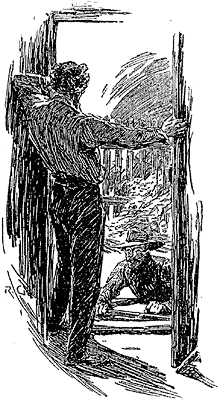
\includegraphics{images/study10-stud-19.png}\end{center}

\noindent \begin{center}\noun{He saw to his astonishment a man lying
flat upon his face upon the ground.}\end{center}
\end{figure}
With a sigh of relief, Ferrier looked to right and to left, until
happening to glance straight down at his own feet he saw to his astonishment
a man lying flat upon his face upon the ground, with arms and legs
all asprawl.

So unnerved was he at the sight that he leaned up against the wall
with his hand to his throat to stifle his inclination to call out.
His first thought was that the prostrate figure was that of some wounded
or dying man, but as he watched it he saw it writhe along the ground
and into the hall with the rapidity and noiselessness of a serpent.
Once within the house the man sprang to his feet, closed the door,
and revealed to the astonished farmer the fierce face and resolute
expression of Jefferson Hope.

{}``Good God!''\ gasped John Ferrier. {}``How you scared me! Whatever
made you come in like that.''

{}``Give me food,'' the other said, hoarsely. {}``I have had no
time for bite or sup for eight-and-forty hours.'' He flung himself
upon the cold meat and bread which were still lying upon the table
from his host's supper, and devoured it voraciously. {}``Does Lucy
bear up well?''\ he asked, when he had satisfied his hunger.

{}``Yes. She does not know the danger,'' her father answered.

{}``That is well. The house is watched on every side. That is why
I crawled my way up to it. They may be darned sharp, but they're not
quite sharp enough to catch a Washoe hunter.''

John Ferrier felt a different man now that he realized that he had
a devoted ally. He seized the young man's leathery hand and wrung
it cordially. {}``You're a man to be proud of,'' he said. {}``There
are not many who would come to share our danger and our troubles.''

{}``You've hit it there, pard,'' the young hunter answered. {}``I
have a respect for you, but if you were alone in this business I'd
think twice before I put my head into such a hornet's nest. It's Lucy
that brings me here, and before harm comes on her I guess there will
be one less o' the Hope family in Utah.''

{}``What are we to do?''

{}``To-morrow is your last day, and unless you act to-night you are
lost. I have a mule and two horses waiting in the Eagle Ravine. How
much money have you?''

{}``Two thousand dollars in gold, and five in notes.''

{}``That will do. I have as much more to add to it. We must push
for Carson City through the mountains. You had best wake Lucy. It
is as well that the servants do not sleep in the house.''

While Ferrier was absent, preparing his daughter for the approaching
journey, Jefferson Hope packed all the eatables that he could find
into a small parcel, and filled a stoneware jar with water, for he
knew by experience that the mountain wells were few and far between.
He had hardly completed his arrangements before the farmer returned
with his daughter all dressed and ready for a start. The greeting
between the lovers was warm, but brief, for minutes were precious,
and there was much to be done.

{}``We must make our start at once,'' said Jefferson Hope, speaking
in a low but resolute voice, like one who realizes the greatness of
the peril, but has steeled his heart to meet it. {}``The front and
back entrances are watched, but with caution we may get away through
the side window and across the fields. Once on the road we are only
two miles from the Ravine where the horses are waiting. By daybreak
we should be half-way through the mountains.''

{}``What if we are stopped,'' asked Ferrier.

Hope slapped the revolver butt which protruded from the front of his
tunic. {}``If they are too many for us we shall take two or three
of them with us,'' he said with a sinister smile.

The lights inside the house had all been extinguished, and from the
darkened window Ferrier peered over the fields which had been his
own, and which he was now about to abandon for ever. He had long nerved
himself to the sacrifice, however, and the thought of the honour and
happiness of his daughter outweighed any regret at his ruined fortunes.
All looked so peaceful and happy, the rustling trees and the broad
silent stretch of grain-land, that it was difficult to realize that
the spirit of murder lurked through it all. Yet the white face and
set expression of the young hunter showed that in his approach to
the house he had seen enough to satisfy him upon that head.

Ferrier carried the bag of gold and notes, Jefferson Hope had the
scanty provisions and water, while Lucy had a small bundle containing
a few of her more valued possessions. Opening the window very slowly
and carefully, they waited until a dark cloud had somewhat obscured
the night, and then one by one passed through into the little garden.
With bated breath and crouching figures they stumbled across it, and
gained the shelter of the hedge, which they skirted until they came
to the gap which opened into the cornfields. They had just reached
this point when the young man seized his two companions and dragged
them down into the shadow, where they lay silent and trembling.

It was as well that his prairie training had given Jefferson Hope
the ears of a lynx. He and his friends had hardly crouched down before
the melancholy hooting of a mountain owl was heard within a few yards
of them, which was immediately answered by another hoot at a small
distance. At the same moment a vague shadowy figure emerged from the
gap for which they had been making, and uttered the plaintive signal
cry again, on which a second man appeared out of the obscurity.

{}``To-morrow at midnight,'' said the first who appeared to be in
authority. {}``When the Whip-poor-Will calls three times.''

{}``It is well,'' returned the other. {}``Shall I tell Brother
Drebber?''

%
\begin{figure}[htbp]
\noindent \begin{center}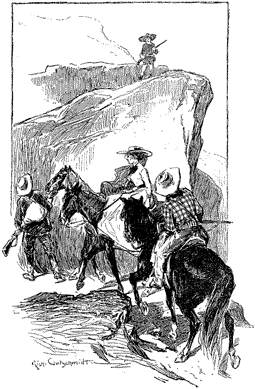
\includegraphics{images/study10-stud-20.png}\end{center}

\noindent \begin{center}\noun{{}``Nine to seven!''\ cried the
sentinel.}\end{center}
\end{figure}
{}``Pass it on to him, and from him to the others. Nine to seven!''

{}``Seven to five!'' repeated the other, and the two figures flitted
away in different directions. Their concluding words had evidently
been some form of sign and countersign. The instant that their footsteps
had died away in the distance, Jefferson Hope sprang to his feet,
and helping his companions through the gap, led the way across the
fields at the top of his speed, supporting and half-carrying the girl
when her strength appeared to fail her.

{}``Hurry on! hurry on!'' he gasped from time to time. {}``We are
through the line of sentinels. Everything depends on speed. Hurry
on!''

Once on the high road they made rapid progress. Only once did they
meet anyone, and then they managed to slip into a field, and so avoid
recognition. Before reaching the town the hunter branched away into
a rugged and narrow footpath which led to the mountains. Two dark
jagged peaks loomed above them through the darkness, and the defile
which led between them was the Eagle Canon in which the horses were
awaiting them. With unerring instinct Jefferson Hope picked his way
among the great boulders and along the bed of a dried-up watercourse,
until he came to the retired corner, screened with rocks, where the
faithful animals had been picketed. The girl was placed upon the mule,
and old Ferrier upon one of the horses, with his money-bag, while
Jefferson Hope led the other along the precipitous and dangerous path.

It was a bewildering route for anyone who was not accustomed to face
Nature in her wildest moods. On the one side a great crag towered
up a thousand feet or more, black, stern, and menacing, with long
basaltic columns upon its rugged surface like the ribs of some petrified
monster. On the other hand a wild chaos of boulders and debris made
all advance impossible. Between the two ran the irregular track, so
narrow in places that they had to travel in Indian file, and so rough
that only practised riders could have traversed it at all. Yet in
spite of all dangers and difficulties, the hearts of the fugitives
were light within them, for every step increased the distance between
them and the terrible despotism from which they were flying.

They soon had a proof, however, that they were still within the jurisdiction
of the Saints. They had reached the very wildest and most desolate
portion of the pass when the girl gave a startled cry, and pointed
upwards. On a rock which overlooked the track, showing out dark and
plain against the sky, there stood a solitary sentinel. He saw them
as soon as they perceived him, and his military challenge of {}``Who
goes there?''\ rang through the silent ravine.

{}``Travellers for Nevada,'' said Jefferson Hope, with his hand
upon the rifle which hung by his saddle.

They could see the lonely watcher fingering his gun, and peering down
at them as if dissatisfied at their reply.

{}``By whose permission?'' he asked.

{}``The Holy Four,'' answered Ferrier. His Mormon experiences had
taught him that that was the highest authority to which he could refer.

{}``Nine from seven,'' cried the sentinel.

{}``Seven from five,'' returned Jefferson Hope promptly, remembering
the countersign which he had heard in the garden.

{}``Pass, and the Lord go with you,'' said the voice from above.
Beyond his post the path broadened out, and the horses were able to
break into a trot. Looking back, they could see the solitary watcher
leaning upon his gun, and knew that they had passed the outlying post
of the chosen people, and that freedom lay before them.


\chapter*{\raggedright CHAPTER V. THE AVENGING ANGELS.}

\addcontentsline{toc}{chapter}{CHAPTER V. THE AVENGING ANGELS.}

\markboth{A STUDY IN SCARLET}{CHAPTER V}

All night their course lay through intricate defiles and over irregular
and rock-strewn paths. More than once they lost their way, but Hope's
intimate knowledge of the mountains enabled them to regain the track
once more. When morning broke, a scene of marvellous though savage
beauty lay before them. In every direction the great snow-capped peaks
hemmed them in, peeping over each other's shoulders to the far horizon.
So steep were the rocky banks on either side of them, that the larch
and the pine seemed to be suspended over their heads, and to need
only a gust of wind to come hurtling down upon them. Nor was the fear
entirely an illusion, for the barren valley was thickly strewn with
trees and boulders which had fallen in a similar manner. Even as they
passed, a great rock came thundering down with a hoarse rattle which
woke the echoes in the silent gorges, and startled the weary horses
into a gallop.

As the sun rose slowly above the eastern horizon, the caps of the
great mountains lit up one after the other, like lamps at a festival,
until they were all ruddy and glowing. The magnificent spectacle cheered
the hearts of the three fugitives and gave them fresh energy. At a
wild torrent which swept out of a ravine they called a halt and watered
their horses, while they partook of a hasty breakfast. Lucy and her
father would fain have rested longer, but Jefferson Hope was inexorable.
{}``They will be upon our track by this time,'' he said. {}``Everything
depends upon our speed. Once safe in Carson we may rest for the remainder
of our lives.''

During the whole of that day they struggled on through the defiles,
and by evening they calculated that they were more than thirty miles
from their enemies. At night-time they chose the base of a beetling
crag, where the rocks offered some protection from the chill wind,
and there huddled together for warmth, they enjoyed a few hours' sleep.
Before daybreak, however, they were up and on their way once more.
They had seen no signs of any pursuers, and Jefferson Hope began to
think that they were fairly out of the reach of the terrible organization
whose enmity they had incurred. He little knew how far that iron grasp
could reach, or how soon it was to close upon them and crush them.

About the middle of the second day of their flight their scanty store
of provisions began to run out. This gave the hunter little uneasiness,
however, for there was game to be had among the mountains, and he
had frequently before had to depend upon his rifle for the needs of
life. Choosing a sheltered nook, he piled together a few dried branches
and made a blazing fire, at which his companions might warm themselves,
for they were now nearly five thousand feet above the sea level, and
the air was bitter and keen. Having tethered the horses, and bade
Lucy adieu, he threw his gun over his shoulder, and set out in search
of whatever chance might throw in his way. Looking back he saw the
old man and the young girl crouching over the blazing fire, while
the three animals stood motionless in the back-ground. Then the intervening
rocks hid them from his view.

He walked for a couple of miles through one ravine after another without
success, though from the marks upon the bark of the trees, and other
indications, he judged that there were numerous bears in the vicinity.
At last, after two or three hours' fruitless search, he was thinking
of turning back in despair, when casting his eyes upwards he saw a
sight which sent a thrill of pleasure through his heart. On the edge
of a jutting pinnacle, three or four hundred feet above him, there
stood a creature somewhat resembling a sheep in appearance, but armed
with a pair of gigantic horns. The big-horn\mdsh{---}for so it is
called\mdsh{---}was acting, probably, as a guardian over a flock
which were invisible to the hunter; but fortunately it was heading
in the opposite direction, and had not perceived him. Lying on his
face, he rested his rifle upon a rock, and took a long and steady
aim before drawing the trigger. The animal sprang into the air, tottered
for a moment upon the edge of the precipice, and then came crashing
down into the valley beneath.

The creature was too unwieldy to lift, so the hunter contented himself
with cutting away one haunch and part of the flank. With this trophy
over his shoulder, he hastened to retrace his steps, for the evening
was already drawing in. He had hardly started, however, before he
realized the difficulty which faced him. In his eagerness he had wandered
far past the ravines which were known to him, and it was no easy matter
to pick out the path which he had taken. The valley in which he found
himself divided and sub-divided into many gorges, which were so like
each other that it was impossible to distinguish one from the other.
He followed one for a mile or more until he came to a mountain torrent
which he was sure that he had never seen before. Convinced that he
had taken the wrong turn, he tried another, but with the same result.
Night was coming on rapidly, and it was almost dark before he at last
found himself in a defile which was familiar to him. Even then it
was no easy matter to keep to the right track, for the moon had not
yet risen, and the high cliffs on either side made the obscurity more
profound. Weighed down with his burden, and weary from his exertions,
he stumbled along, keeping up his heart by the reflection that every
step brought him nearer to Lucy, and that he carried with him enough
to ensure them food for the remainder of their journey.

He had now come to the mouth of the very defile in which he had left
them. Even in the darkness he could recognize the outline of the cliffs
which bounded it. They must, he reflected, be awaiting him anxiously,
for he had been absent nearly five hours. In the gladness of his heart
he put his hands to his mouth and made the glen re-echo to a loud
halloo as a signal that he was coming. He paused and listened for
an answer. None came save his own cry, which clattered up the dreary
silent ravines, and was borne back to his ears in countless repetitions.
Again he shouted, even louder than before, and again no whisper came
back from the friends whom he had left such a short time ago. A vague,
nameless dread came over him, and he hurried onwards frantically,
dropping the precious food in his agitation.

When he turned the corner, he came full in sight of the spot where
the fire had been lit. There was still a glowing pile of wood ashes
there, but it had evidently not been tended since his departure. The
same dead silence still reigned all round. With his fears all changed
to convictions, he hurried on. There was no living creature near the
remains of the fire: animals, man, maiden, all were gone. It was only
too clear that some sudden and terrible disaster had occurred during
his absence\mdsh{---}a disaster which had embraced them all, and
yet had left no traces behind it.

Bewildered and stunned by this blow, Jefferson Hope felt his head
spin round, and had to lean upon his rifle to save himself from falling.
He was essentially a man of action, however, and speedily recovered
from his temporary impotence. Seizing a half-consumed piece of wood
from the smouldering fire, he blew it into a flame, and proceeded
with its help to examine the little camp. The ground was all stamped
down by the feet of horses, showing that a large party of mounted
men had overtaken the fugitives, and the direction of their tracks
proved that they had afterwards turned back to Salt Lake City. Had
they carried back both of his companions with them? Jefferson Hope
had almost persuaded himself that they must have done so, when his
eye fell upon an object which made every nerve of his body tingle
within him. A little way on one side of the camp was a low-lying heap
of reddish soil, which had assuredly not been there before. There
was no mistaking it for anything but a newly-dug grave. As the young
hunter approached it, he perceived that a stick had been planted on
it, with a sheet of paper stuck in the cleft fork of it. %
\begin{figure}[htbp]
\noindent \begin{center}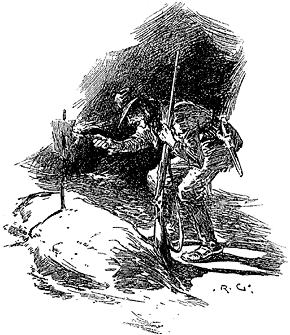
\includegraphics[%
  width=1.0\columnwidth]{images/study10-stud-21.png}\end{center}

\noindent \begin{center}\noun{{}``John Ferrier, formerly of Salt
Lake City. Died August 4th, 1860.''}\end{center}
\end{figure}
The inscription upon the paper was brief, but to the point:

\begin{center} \sc

JOHN FERRIER, \\*

\small FORMERLY OF SALT LAKE CITY, \\*

Died August 4th, 1860.

\end{center}

The sturdy old man, whom he had left so short a time before, was gone,
then, and this was all his epitaph. Jefferson Hope looked wildly round
to see if there was a second grave, but there was no sign of one.
Lucy had been carried back by their terrible pursuers to fulfil her
original destiny, by becoming one of the harem of the Elder's son.
As the young fellow realized the certainty of her fate, and his own
powerlessness to prevent it, he wished that he, too, was lying with
the old farmer in his last silent resting-place.

Again, however, his active spirit shook off the lethargy which springs
from despair. If there was nothing else left to him, he could at least
devote his life to revenge. With indomitable patience and perseverance,
Jefferson Hope possessed also a power of sustained vindictiveness,
which he may have learned from the Indians amongst whom he had lived.
As he stood by the desolate fire, he felt that the only one thing
which could assuage his grief would be thorough and complete retribution,
brought by his own hand upon his enemies. His strong will and untiring
energy should, he determined, be devoted to that one end. With a grim,
white face, he retraced his steps to where he had dropped the food,
and having stirred up the smouldering fire, he cooked enough to last
him for a few days. This he made up into a bundle, and, tired as he
was, he set himself to walk back through the mountains upon the track
of the avenging angels.

For five days he toiled footsore and weary through the defiles which
he had already traversed on horseback. At night he flung himself down
among the rocks, and snatched a few hours of sleep; but before daybreak
he was always well on his way. On the sixth day, he reached the Eagle
Ca�on, from which they had commenced their ill-fated flight. Thence
he could look down upon the home of the saints. Worn and exhausted,
he leaned upon his rifle and shook his gaunt hand fiercely at the
silent widespread city beneath him. As he looked at it, he observed
that there were flags in some of the principal streets, and other
signs of festivity. He was still speculating as to what this might
mean when he heard the clatter of horse's hoofs, and saw a mounted
man riding towards him. As he approached, he recognized him as a Mormon
named Cowper, to whom he had rendered services at different times.
He therefore accosted him when he got up to him, with the object of
finding out what Lucy Ferrier's fate had been.

{}``I am Jefferson Hope,'' he said. {}``You remember me.''

The Mormon looked at him with undisguised astonishment\mdsh{---}indeed,
it was difficult to recognize in this tattered, unkempt wanderer,
with ghastly white face and fierce, wild eyes, the spruce young hunter
of former days. Having, however, at last, satisfied himself as to
his identity, the man's surprise changed to consternation.

{}``You are mad to come here,'' he cried. {}``It is as much as
my own life is worth to be seen talking with you. There is a warrant
against you from the Holy Four for assisting the Ferriers away.''

{}``I don't fear them, or their warrant,'' Hope said, earnestly.
{}``You must know something of this matter, Cowper. I conjure you
by everything you hold dear to answer a few questions. We have always
been friends. For God's sake, don't refuse to answer me.''

{}``What is it?''\ the Mormon asked uneasily. {}``Be quick. The
very rocks have ears and the trees eyes.''

{}``What has become of Lucy Ferrier?''

{}``She was married yesterday to young Drebber. Hold up, man, hold
up, you have no life left in you.''

{}``Don't mind me,'' said Hope faintly. He was white to the very
lips, and had sunk down on the stone against which he had been leaning.
{}``Married, you say?''

{}``Married yesterday\mdsh{---}that's what those flags are for on
the Endowment House. There was some words between young Drebber and
young Stangerson as to which was to have her. They'd both been in
the party that followed them, and Stangerson had shot her father,
which seemed to give him the best claim; but when they argued it out
in council, Drebber's party was the stronger, so the Prophet gave
her over to him. No one won't have her very long though, for I saw
death in her face yesterday. She is more like a ghost than a woman.
Are you off, then?''

{}``Yes, I am off,'' said Jefferson Hope, who had risen from his
seat. His face might have been chiselled out of marble, so hard and
set was its expression, while its eyes glowed with a baleful light.

{}``Where are you going?''

{}``Never mind,'' he answered; and, slinging his weapon over his
shoulder, strode off down the gorge and so away into the heart of
the mountains to the haunts of the wild beasts. Amongst them all there
was none so fierce and so dangerous as himself.

The prediction of the Mormon was only too well fulfilled. Whether
it was the terrible death of her father or the effects of the hateful
marriage into which she had been forced, poor Lucy never held up her
head again, but pined away and died within a month. Her sottish husband,
who had married her principally for the sake of John Ferrier's property,
did not affect any great grief at his bereavement; but his other wives
mourned over her, and sat up with her the night before the burial,
as is the Mormon custom. They were grouped round the bier in the early
hours of the morning, when, to their inexpressible fear and astonishment,
the door was flung open, and a savage-looking, weather-beaten man
in tattered garments strode into the room. Without a glance or a word
to the cowering women, he walked up to the white silent figure which
had once contained the pure soul of Lucy Ferrier. Stooping over her,
he pressed his lips reverently to her cold forehead, and then, snatching
up her hand, he took the wedding-ring from her finger. {}``She shall
not be buried in that,'' he cried with a fierce snarl, and before
an alarm could be raised sprang down the stairs and was gone. So strange
and so brief was the episode, that the watchers might have found it
hard to believe it themselves or persuade other people of it, had
it not been for the undeniable fact that the circlet of gold which
marked her as having been a bride had disappeared.

For some months Jefferson Hope lingered among the mountains, leading
a strange wild life, and nursing in his heart the fierce desire for
vengeance which possessed him. Tales were told in the City of the
weird figure which was seen prowling about the suburbs, and which
haunted the lonely mountain gorges. Once a bullet whistled through
Stangerson's window and flattened itself upon the wall within a foot
of him. On another occasion, as Drebber passed under a cliff a great
boulder crashed down on him, and he only escaped a terrible death
by throwing himself upon his face. The two young Mormons were not
long in discovering the reason of these attempts upon their lives,
and led repeated expeditions into the mountains in the hope of capturing
or killing their enemy, but always without success. Then they adopted
the precaution of never going out alone or after nightfall, and of
having their houses guarded. After a time they were able to relax
these measures, for nothing was either heard or seen of their opponent,
and they hoped that time had cooled his vindictiveness.

Far from doing so, it had, if anything, augmented it. The hunter's
mind was of a hard, unyielding nature, and the predominant idea of
revenge had taken such complete possession of it that there was no
room for any other emotion. He was, however, above all things practical.
He soon realized that even his iron constitution could not stand the
incessant strain which he was putting upon it. Exposure and want of
wholesome food were wearing him out. If he died like a dog among the
mountains, what was to become of his revenge then? And yet such a
death was sure to overtake him if he persisted. He felt that that
was to play his enemy's game, so he reluctantly returned to the old
Nevada mines, there to recruit his health and to amass money enough
to allow him to pursue his object without privation.

His intention had been to be absent a year at the most, but a combination
of unforeseen circumstances prevented his leaving the mines for nearly
five. At the end of that time, however, his memory of his wrongs and
his craving for revenge were quite as keen as on that memorable night
when he had stood by John Ferrier's grave. Disguised, and under an
assumed name, he returned to Salt Lake City, careless what became
of his own life, as long as he obtained what he knew to be justice.
There he found evil tidings awaiting him. There had been a schism
among the Chosen People a few months before, some of the younger members
of the Church having rebelled against the authority of the Elders,
and the result had been the secession of a certain number of the malcontents,
who had left Utah and become Gentiles. Among these had been Drebber
and Stangerson; and no one knew whither they had gone. Rumour reported
that Drebber had managed to convert a large part of his property into
money, and that he had departed a wealthy man, while his companion,
Stangerson, was comparatively poor. There was no clue at all, however,
as to their whereabouts.

Many a man, however vindictive, would have abandoned all thought of
revenge in the face of such a difficulty, but Jefferson Hope never
faltered for a moment. With the small competence he possessed, eked
out by such employment as he could pick up, he travelled from town
to town through the United States in quest of his enemies. Year passed
into year, his black hair turned grizzled, but still he wandered on,
a human bloodhound, with his mind wholly set upon the one object upon
which he had devoted his life. At last his perseverance was rewarded.
It was but a glance of a face in a window, but that one glance told
him that Cleveland in Ohio possessed the men whom he was in pursuit
of. He returned to his miserable lodgings with his plan of vengeance
all arranged. It chanced, however, that Drebber, looking from his
window, had recognized the vagrant in the street, and had read murder
in his eyes. He hurried before a justice of the peace, accompanied
by Stangerson, who had become his private secretary, and represented
to him that they were in danger of their lives from the jealousy and
hatred of an old rival. That evening Jefferson Hope was taken into
custody, and not being able to find sureties, was detained for some
weeks. When at last he was liberated, it was only to find that Drebber's
house was deserted, and that he and his secretary had departed for
Europe.

Again the avenger had been foiled, and again his concentrated hatred
urged him to continue the pursuit. Funds were wanting, however, and
for some time he had to return to work, saving every dollar for his
approaching journey. At last, having collected enough to keep life
in him, he departed for Europe, and tracked his enemies from city
to city, working his way in any menial capacity, but never overtaking
the fugitives. When he reached St.\ Petersburg they had departed
for Paris; and when he followed them there he learned that they had
just set off for Copenhagen. At the Danish capital he was again a
few days late, for they had journeyed on to London, where he at last
succeeded in running them to earth. As to what occurred there, we
cannot do better than quote the old hunter's own account, as duly
recorded in Dr.\ Watson's Journal, to which we are already under
such obligations.


\chapter*{\raggedright CHAPTER VI. A CONTINUATION OF THE REMINISCENCES OF
JOHN WATSON, M.D.}

\addcontentsline{toc}{chapter}{CHAPTER VI. A CONTINUATION OF THE
\\
REMINISCENCES OF JOHN\\
WATSON, M.D.}

\markboth{A STUDY IN SCARLET}{CHAPTER VI}

Our prisoner's furious resistance did not apparently indicate any
ferocity in his disposition towards ourselves, for on finding himself
powerless, he smiled in an affable manner, and expressed his hopes
that he had not hurt any of us in the scuffle. {}``I guess you're
going to take me to the police-station,'' he remarked to Sherlock
Holmes. {}``My cab's at the door. If you'll loose my legs I'll walk
down to it. I'm not so light to lift as I used to be.''

Gregson and Lestrade exchanged glances as if they thought this proposition
rather a bold one; but Holmes at once took the prisoner at his word,
and loosened the towel which we had bound round his ankles. He rose
and stretched his legs, as though to assure himself that they were
free once more. I remember that I thought to myself, as I eyed him,
that I had seldom seen a more powerfully built man; and his dark sunburned
face bore an expression of determination and energy which was as formidable
as his personal strength.

{}``If there's a vacant place for a chief of the police, I reckon
you are the man for it,'' he said, gazing with undisguised admiration
at my fellow-lodger. {}``The way you kept on my trail was a caution.''

{}``You had better come with me,'' said Holmes to the two detectives.

{}``I can drive you,'' said Lestrade.

{}``Good!\ and Gregson can come inside with me. You too, Doctor,
you have taken an interest in the case and may as well stick to us.''

I assented gladly, and we all descended together. Our prisoner made
no attempt at escape, but stepped calmly into the cab which had been
his, and we followed him. Lestrade mounted the box, whipped up the
horse, and brought us in a very short time to our destination. We
were ushered into a small chamber where a police Inspector noted down
our prisoner's name and the names of the men with whose murder he
had been charged. The official was a white-faced unemotional man,
who went through his duties in a dull mechanical way. {}``The prisoner
will be put before the magistrates in the course of the week,'' he
said; {}``in the mean time, Mr. Jefferson Hope, have you anything
that you wish to say? I must warn you that your words will be taken
down, and may be used against you.''

%
\begin{figure}[htbp]
\noindent \begin{center}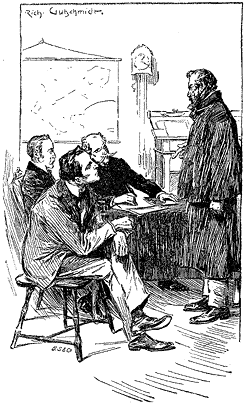
\includegraphics{images/study10-stud-22.png}\end{center}

\noindent \begin{center}\noun{{}``I've got a good deal to say,''
our prisoner said slowly.}\end{center}
\end{figure}
{}``I've got a good deal to say,'' our prisoner said slowly. {}``I
want to tell you gentlemen all about it.''

{}``Hadn't you better reserve that for your trial?'' asked the Inspector.

{}``I may never be tried,'' he answered. {}``You needn't look startled.
It isn't suicide I am thinking of. Are you a Doctor?'' He turned
his fierce dark eyes upon me as he asked this last question.

{}``Yes; I am,'' I answered.

{}``Then put your hand here,'' he said, with a smile, motioning
with his manacled wrists towards his chest.

I did so; and became at once conscious of an extraordinary throbbing
and commotion which was going on inside. The walls of his chest seemed
to thrill and quiver as a frail building would do inside when some
powerful engine was at work. In the silence of the room I could hear
a dull humming and buzzing noise which proceeded from the same source.

{}``Why,'' I cried, {}``you have an aortic aneurism!''

{}``That's what they call it,'' he said, placidly. {}``I went to
a Doctor last week about it, and he told me that it is bound to burst
before many days passed. It has been getting worse for years. I got
it from over-exposure and under-feeding among the Salt Lake Mountains.
I've done my work now, and I don't care how soon I go, but I should
like to leave some account of the business behind me. I don't want
to be remembered as a common cut-throat.''

The Inspector and the two detectives had a hurried discussion as to
the advisability of allowing him to tell his story.

{}``Do you consider, Doctor, that there is immediate danger?'' the
former asked.

{}``Most certainly there is,'' I answered.

{}``In that case it is clearly our duty, in the interests of justice,
to take his statement,'' said the Inspector. {}``You are at liberty,
sir, to give your account, which I again warn you will be taken down.''

{}``I'll sit down, with your leave,'' the prisoner said, suiting
the action to the word. {}``This aneurism of mine makes me easily
tired, and the tussle we had half an hour ago has not mended matters.
I'm on the brink of the grave, and I am not likely to lie to you.
Every word I say is the absolute truth, and how you use it is a matter
of no consequence to me.''

With these words, Jefferson Hope leaned back in his chair and began
the following remarkable statement. He spoke in a calm and methodical
manner, as though the events which he narrated were commonplace enough.
I can vouch for the accuracy of the subjoined account, for I have
had access to Lestrade's note-book, in which the prisoner's words
were taken down exactly as they were uttered.

{}``It don't much matter to you why I hated these men,'' he said;
{}``it's enough that they were guilty of the death of two human beings\mdsh{---}a
father and a daughter\mdsh{---}and that they had, therefore, forfeited
their own lives. After the lapse of time that has passed since their
crime, it was impossible for me to secure a conviction against them
in any court. I knew of their guilt though, and I determined that
I should be judge, jury, and executioner all rolled into one. You'd
have done the same, if you have any manhood in you, if you had been
in my place.

{}``That girl that I spoke of was to have married me twenty years
ago. She was forced into marrying that same Drebber, and broke her
heart over it. I took the marriage ring from her dead finger, and
I vowed that his dying eyes should rest upon that very ring, and that
his last thoughts should be of the crime for which he was punished.
I have carried it about with me, and have followed him and his accomplice
over two continents until I caught them. They thought to tire me out,
but they could not do it. If I die to-morrow, as is likely enough,
I die knowing that my work in this world is done, and well done. They
have perished, and by my hand. There is nothing left for me to hope
for, or to desire.

{}``They were rich and I was poor, so that it was no easy matter
for me to follow them. When I got to London my pocket was about empty,
and I found that I must turn my hand to something for my living. Driving
and riding are as natural to me as walking, so I applied at a cabowner's
office, and soon got employment. I was to bring a certain sum a week
to the owner, and whatever was over that I might keep for myself.
There was seldom much over, but I managed to scrape along somehow.
The hardest job was to learn my way about, for I reckon that of all
the mazes that ever were contrived, this city is the most confusing.
I had a map beside me though, and when once I had spotted the principal
hotels and stations, I got on pretty well.

{}``It was some time before I found out where my two gentlemen were
living; but I inquired and inquired until at last I dropped across
them. They were at a boarding-house at Camberwell, over on the other
side of the river. When once I found them out I knew that I had them
at my mercy. I had grown my beard, and there was no chance of their
recognizing me. I would dog them and follow them until I saw my opportunity.
I was determined that they should not escape me again.

{}``They were very near doing it for all that. Go where they would
about London, I was always at their heels. Sometimes I followed them
on my cab, and sometimes on foot, but the former was the best, for
then they could not get away from me. It was only early in the morning
or late at night that I could earn anything, so that I began to get
behind hand with my employer. I did not mind that, however, as long
as I could lay my hand upon the men I wanted.

{}``They were very cunning, though. They must have thought that there
was some chance of their being followed, for they would never go out
alone, and never after nightfall. During two weeks I drove behind
them every day, and never once saw them separate. Drebber himself
was drunk half the time, but Stangerson was not to be caught napping.
I watched them late and early, but never saw the ghost of a chance;
but I was not discouraged, for something told me that the hour had
almost come. My only fear was that this thing in my chest might burst
a little too soon and leave my work undone.

{}``At last, one evening I was driving up and down Torquay Terrace,
as the street was called in which they boarded, when I saw a cab drive
up to their door. Presently some luggage was brought out, and after
a time Drebber and Stangerson followed it, and drove off. I whipped
up my horse and kept within sight of them, feeling very ill at ease,
for I feared that they were going to shift their quarters. At Euston
Station they got out, and I left a boy to hold my horse, and followed
them on to the platform. I heard them ask for the Liverpool train,
and the guard answer that one had just gone and there would not be
another for some hours. Stangerson seemed to be put out at that, but
Drebber was rather pleased than otherwise. I got so close to them
in the bustle that I could hear every word that passed between them.
Drebber said that he had a little business of his own to do, and that
if the other would wait for him he would soon rejoin him. His companion
remonstrated with him, and reminded him that they had resolved to
stick together. Drebber answered that the matter was a delicate one,
and that he must go alone. I could not catch what Stangerson said
to that, but the other burst out swearing, and reminded him that he
was nothing more than his paid servant, and that he must not presume
to dictate to him. On that the Secretary gave it up as a bad job,
and simply bargained with him that if he missed the last train he
should rejoin him at Halliday's Private Hotel; to which Drebber answered
that he would be back on the platform before eleven, and made his
way out of the station.

{}``The moment for which I had waited so long had at last come. I
had my enemies within my power. Together they could protect each other,
but singly they were at my mercy. I did not act, however, with undue
precipitation. My plans were already formed. There is no satisfaction
in vengeance unless the offender has time to realize who it is that
strikes him, and why retribution has come upon him. I had my plans
arranged by which I should have the opportunity of making the man
who had wronged me understand that his old sin had found him out.
It chanced that some days before a gentleman who had been engaged
in looking over some houses in the Brixton Road had dropped the key
of one of them in my carriage. It was claimed that same evening, and
returned; but in the interval I had taken a moulding of it, and had
a duplicate constructed. By means of this I had access to at least
one spot in this great city where I could rely upon being free from
interruption. How to get Drebber to that house was the difficult problem
which I had now to solve.

{}``He walked down the road and went into one or two liquor shops,
staying for nearly half-an-hour in the last of them. When he came
out he staggered in his walk, and was evidently pretty well on. There
was a hansom just in front of me, and he hailed it. I followed it
so close that the nose of my horse was within a yard of his driver
the whole way. We rattled across Waterloo Bridge and through miles
of streets, until, to my astonishment, we found ourselves back in
the Terrace in which he had boarded. I could not imagine what his
intention was in returning there; but I went on and pulled up my cab
a hundred yards or so from the house. He entered it, and his hansom
drove away. Give me a glass of water, if you please. My mouth gets
dry with the talking.''

I handed him the glass, and he drank it down.

{}``That's better,'' he said. {}``Well, I waited for a quarter
of an hour, or more, when suddenly there came a noise like people
struggling inside the house. Next moment the door was flung open and
two men appeared, one of whom was Drebber, and the other was a young
chap whom I had never seen before. This fellow had Drebber by the
collar, and when they came to the head of the steps he gave him a
shove and a kick which sent him half across the road.\  `You hound,'
he cried, shaking his stick at him; `I'll teach you to insult an honest
girl!' He was so hot that I think he would have thrashed Drebber with
his cudgel, only that the cur staggered away down the road as fast
as his legs would carry him. He ran as far as the corner, and then,
seeing my cab, he hailed me and jumped in.\  `Drive me to Halliday's
Private Hotel,' said he.

{}``When I had him fairly inside my cab, my heart jumped so with
joy that I feared lest at this last moment my aneurism might go wrong.
I drove along slowly, weighing in my own mind what it was best to
do. I might take him right out into the country, and there in some
deserted lane have my last interview with him. I had almost decided
upon this, when he solved the problem for me. The craze for drink
had seized him again, and he ordered me to pull up outside a gin palace.
He went in, leaving word that I should wait for him. There he remained
until closing time, and when he came out he was so far gone that I
knew the game was in my own hands.

{}``Don't imagine that I intended to kill him in cold blood. It would
only have been rigid justice if I had done so, but I could not bring
myself to do it. I had long determined that he should have a show
for his life if he chose to take advantage of it. Among the many billets
which I have filled in America during my wandering life, I was once
janitor and sweeper out of the laboratory at York College. One day
the professor was lecturing on poisons, and he showed his students
some alkaloid, as he called it, which he had extracted from some South
American arrow poison, and which was so powerful that the least grain
meant instant death. I spotted the bottle in which this preparation
was kept, and when they were all gone, I helped myself to a little
of it. I was a fairly good dispenser, so I worked this alkaloid into
small, soluble pills, and each pill I put in a box with a similar
pill made without the poison. I determined at the time that when I
had my chance, my gentlemen should each have a draw out of one of
these boxes, while I ate the pill that remained. It would be quite
as deadly, and a good deal less noisy than firing across a handkerchief.
From that day I had always my pill boxes about with me, and the time
had now come when I was to use them.

{}``It was nearer one than twelve, and a wild, bleak night, blowing
hard and raining in torrents. Dismal as it was outside, I was glad
within\mdsh{---}so glad that I could have shouted out from pure exultation.
If any of you gentlemen have ever pined for a thing, and longed for
it during twenty long years, and then suddenly found it within your
reach, you would understand my feelings. I lit a cigar, and puffed
at it to steady my nerves, but my hands were trembling, and my temples
throbbing with excitement. As I drove, I could see old John Ferrier
and sweet Lucy looking at me out of the darkness and smiling at me,
just as plain as I see you all in this room. All the way they were
ahead of me, one on each side of the horse until I pulled up at the
house in the Brixton Road.

{}``There was not a soul to be seen, nor a sound to be heard, except
the dripping of the rain. When I looked in at the window, I found
Drebber all huddled together in a drunken sleep. I shook him by the
arm, `It's time to get out,' I said.

{}```All right, cabby,' said he.

{}``I suppose he thought we had come to the hotel that he had mentioned,
for he got out without another word, and followed me down the garden.
I had to walk beside him to keep him steady, for he was still a little
top-heavy. When we came to the door, I opened it, and led him into
the front room. I give you my word that all the way, the father and
the daughter were walking in front of us.

{}```It's infernally dark,' said he, stamping about.

{}```We'll soon have a light,' I said, striking a match and putting
it to a wax candle which I had brought with me. `Now, Enoch Drebber,'
I continued, turning to him, and holding the light to my own face,
`who am I?'

%
\begin{figure}[htbp]
\noindent \begin{center}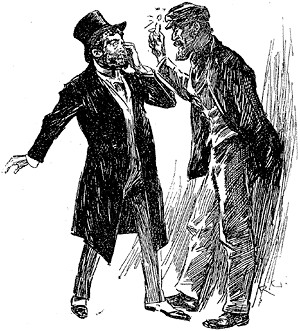
\includegraphics[%
  width=1.0\columnwidth]{images/study10-stud-23.png}\end{center}

\noindent \begin{center}\noun{{}``He gazed at me with bleared,
drunken eyes for a moment, and then I saw a horror spring up in them,
and convulse his whole features, which showed me that he knew me.''}\end{center}
\end{figure}
{}``He gazed at me with bleared, drunken eyes for a moment, and then
I saw a horror spring up in them, and convulse his whole features,
which showed me that he knew me. He staggered back with a livid face,
and I saw the perspiration break out upon his brow, while his teeth
chattered in his head. At the sight, I leaned my back against the
door and laughed loud and long. I had always known that vengeance
would be sweet, but I had never hoped for the contentment of soul
which now possessed me.

{}```You dog!' I said; `I have hunted you from Salt Lake City to
St.\ Petersburg, and you have always escaped me. Now, at last your
wanderings have come to an end, for either you or I shall never see
to-morrow's sun rise.' He shrunk still further away as I spoke, and
I could see on his face that he thought I was mad. So I was for the
time. The pulses in my temples beat like sledge-hammers, and I believe
I would have had a fit of some sort if the blood had not gushed from
my nose and relieved me.

{}```What do you think of Lucy Ferrier now?'\ I cried, locking the
door, and shaking the key in his face.\  `Punishment has been slow
in coming, but it has overtaken you at last.' I saw his coward lips
tremble as I spoke. He would have begged for his life, but he knew
well that it was useless.

{}```Would you murder me?' he stammered.

{}```There is no murder,' I answered.\  `Who talks of murdering
a mad dog? What mercy had you upon my poor darling, when you dragged
her from her slaughtered father, and bore her away to your accursed
and shameless harem.'

{}```It was not I who killed her father,' he cried.

{}```But it was you who broke her innocent heart,' I shrieked, thrusting
the box before him.\  `Let the high God judge between us. Choose
and eat. There is death in one and life in the other. I shall take
what you leave. Let us see if there is justice upon the earth, or
if we are ruled by chance.'

{}``He cowered away with wild cries and prayers for mercy, but I
drew my knife and held it to his throat until he had obeyed me. Then
I swallowed the other, and we stood facing one another in silence
for a minute or more, waiting to see which was to live and which was
to die. Shall I ever forget the look which came over his face when
the first warning pangs told him that the poison was in his system?
I laughed as I saw it, and held Lucy's marriage ring in front of his
eyes. It was but for a moment, for the action of the alkaloid is rapid.
A spasm of pain contorted his features; he threw his hands out in
front of him, staggered, and then, with a hoarse cry, fell heavily
upon the floor. I turned him over with my foot, and placed my hand
upon his heart. There was no movement. He was dead!

{}``The blood had been streaming from my nose, but I had taken no
notice of it. I don't know what it was that put it into my head to
write upon the wall with it. Perhaps it was some mischievous idea
of setting the police upon a wrong track, for I felt light-hearted
and cheerful. I remembered a German being found in New York with RACHE
written up above him, and it was argued at the time in the newspapers
that the secret societies must have done it. I guessed that what puzzled
the New Yorkers would puzzle the Londoners, so I dipped my finger
in my own blood and printed it on a convenient place on the wall.
Then I walked down to my cab and found that there was nobody about,
and that the night was still very wild. I had driven some distance
when I put my hand into the pocket in which I usually kept Lucy's
ring, and found that it was not there. I was thunderstruck at this,
for it was the only memento that I had of her. Thinking that I might
have dropped it when I stooped over Drebber's body, I drove back,
and leaving my cab in a side street, I went boldly up to the house\mdsh{---}for
I was ready to dare anything rather than lose the ring. When I arrived
there, I walked right into the arms of a police-officer who was coming
out, and only managed to disarm his suspicions by pretending to be
hopelessly drunk.

{}``That was how Enoch Drebber came to his end. All I had to do then
was to do as much for Stangerson, and so pay off John Ferrier's debt.
I knew that he was staying at Halliday's Private Hotel, and I hung
about all day, but he never came out. I fancy that he suspected something
when Drebber failed to put in an appearance. He was cunning, was Stangerson,
and always on his guard. If he thought he could keep me off by staying
indoors he was very much mistaken. I soon found out which was the
window of his bedroom, and early next morning I took advantage of
some ladders which were lying in the lane behind the hotel, and so
made my way into his room in the grey of the dawn. I woke him up and
told him that the hour had come when he was to answer for the life
he had taken so long before. I described Drebber's death to him, and
I gave him the same choice of the poisoned pills. Instead of grasping
at the chance of safety which that offered him, he sprang from his
bed and flew at my throat. In self-defence I stabbed him to the heart.
It would have been the same in any case, for Providence would never
have allowed his guilty hand to pick out anything but the poison.

{}``I have little more to say, and it's as well, for I am about done
up. I went on cabbing it for a day or so, intending to keep at it
until I could save enough to take me back to America. I was standing
in the yard when a ragged youngster asked if there was a cabby there
called Jefferson Hope, and said that his cab was wanted by a gentleman
at \noun{221b}, Baker Street. I went round, suspecting no harm,
and the next thing I knew, this young man here had the bracelets on
my wrists, and as neatly shackled as ever I saw in my life. That's
the whole of my story, gentlemen. You may consider me to be a murderer;
but I hold that I am just as much an officer of justice as you are.''

So thrilling had the man's narrative been, and his manner was so impressive
that we had sat silent and absorbed. Even the professional detectives,
\textit{blas�} as they were in every detail of crime, appeared to
be keenly interested in the man's story. When he finished we sat for
some minutes in a stillness which was only broken by the scratching
of Lestrade's pencil as he gave the finishing touches to his shorthand
account.

{}``There is only one point on which I should like a little more
information,'' Sherlock Holmes said at last. {}``Who was your accomplice
who came for the ring which I advertised?''

The prisoner winked at my friend jocosely. {}``I can tell my own
secrets,'' he said, {}``but I don't get other people into trouble.
I saw your advertisement, and I thought it might be a plant, or it
might be the ring which I wanted. My friend volunteered to go and
see. I think you'll own he did it smartly.''

{}``Not a doubt of that,'' said Holmes heartily.

{}``Now, gentlemen,'' the Inspector remarked gravely, {}``the forms
of the law must be complied with. On Thursday the prisoner will be
brought before the magistrates, and your attendance will be required.
Until then I will be responsible for him.'' He rang the bell as he
spoke, and Jefferson Hope was led off by a couple of warders, while
my friend and I made our way out of the Station and took a cab back
to Baker Street.


\chapter*{\raggedright CHAPTER VII. THE CONCLUSION.}

\addcontentsline{toc}{chapter}{CHAPTER VII. THE CONCLUSION.}

\markboth{A STUDY IN SCARLET}{CHAPTER VII}

We had all been warned to appear before the magistrates upon the Thursday;
but when the Thursday came there was no occasion for our testimony.
A higher Judge had taken the matter in hand, and Jefferson Hope had
been summoned before a tribunal where strict justice would be meted
out to him. On the very night after his capture the aneurism burst,
and he was found in the morning stretched upon the floor of the cell,
with a placid smile upon his face, as though he had been able in his
dying moments to look back upon a useful life, and on work well done.

{}``Gregson and Lestrade will be wild about his death,'' Holmes
remarked, as we chatted it over next evening. {}``Where will their
grand advertisement be now?''

{}``I don't see that they had very much to do with his capture,''
I answered.

{}``What you do in this world is a matter of no consequence,'' returned
my companion, bitterly. {}``The question is, what can you make people
believe that you have done. Never mind,'' he continued, more brightly,
after a pause. {}``I would not have missed the investigation for
anything. There has been no better case within my recollection. Simple
as it was, there were several most instructive points about it.''

{}``Simple!'' I ejaculated.

{}``Well, really, it can hardly be described as otherwise,'' said
Sherlock Holmes, smiling at my surprise. {}``The proof of its intrinsic
simplicity is, that without any help save a few very ordinary deductions
I was able to lay my hand upon the criminal within three days.''

{}``That is true,'' said I.

{}``I have already explained to you that what is out of the common
is usually a guide rather than a hindrance. In solving a problem of
this sort, the grand thing is to be able to reason backwards. That
is a very useful accomplishment, and a very easy one, but people do
not practise it much. In the every-day affairs of life it is more
useful to reason forwards, and so the other comes to be neglected.
There are fifty who can reason synthetically for one who can reason
analytically.''

{}``I confess,'' said I, {}``that I do not quite follow you.''

{}``I hardly expected that you would. Let me see if I can make it
clearer. Most people, if you describe a train of events to them, will
tell you what the result would be. They can put those events together
in their minds, and argue from them that something will come to pass.
There are few people, however, who, if you told them a result, would
be able to evolve from their own inner consciousness what the steps
were which led up to that result. This power is what I mean when I
talk of reasoning backwards, or analytically.''

{}``I understand,'' said I.

{}``Now this was a case in which you were given the result and had
to find everything else for yourself. Now let me endeavour to show
you the different steps in my reasoning. To begin at the beginning.
I approached the house, as you know, on foot, and with my mind entirely
free from all impressions. I naturally began by examining the roadway,
and there, as I have already explained to you, I saw clearly the marks
of a cab, which, I ascertained by inquiry, must have been there during
the night. I satisfied myself that it was a cab and not a private
carriage by the narrow gauge of the wheels. The ordinary London growler
is considerably less wide than a gentleman's brougham.

{}``This was the first point gained. I then walked slowly down the
garden path, which happened to be composed of a clay soil, peculiarly
suitable for taking impressions. No doubt it appeared to you to be
a mere trampled line of slush, but to my trained eyes every mark upon
its surface had a meaning. There is no branch of detective science
which is so important and so much neglected as the art of tracing
footsteps. Happily, I have always laid great stress upon it, and much
practice has made it second nature to me. I saw the heavy footmarks
of the constables, but I saw also the track of the two men who had
first passed through the garden. It was easy to tell that they had
been before the others, because in places their marks had been entirely
obliterated by the others coming upon the top of them. In this way
my second link was formed, which told me that the nocturnal visitors
were two in number, one remarkable for his height (as I calculated
from the length of his stride), and the other fashionably dressed,
to judge from the small and elegant impression left by his boots.

{}``On entering the house this last inference was confirmed. My well-booted
man lay before me. The tall one, then, had done the murder, if murder
there was. There was no wound upon the dead man's person, but the
agitated expression upon his face assured me that he had foreseen
his fate before it came upon him. Men who die from heart disease,
or any sudden natural cause, never by any chance exhibit agitation
upon their features. Having sniffed the dead man's lips I detected
a slightly sour smell, and I came to the conclusion that he had had
poison forced upon him. Again, I argued that it had been forced upon
him from the hatred and fear expressed upon his face. By the method
of exclusion, I had arrived at this result, for no other hypothesis
would meet the facts. Do not imagine that it was a very unheard of
idea. The forcible administration of poison is by no means a new thing
in criminal annals. The cases of Dolsky in Odessa, and of Leturier
in Montpellier, will occur at once to any toxicologist.

{}``And now came the great question as to the reason why. Robbery
had not been the object of the murder, for nothing was taken. Was
it politics, then, or was it a woman? That was the question which
confronted me. I was inclined from the first to the latter supposition.
Political assassins are only too glad to do their work and to fly.
This murder had, on the contrary, been done most deliberately, and
the perpetrator had left his tracks all over the room, showing that
he had been there all the time. It must have been a private wrong,
and not a political one, which called for such a methodical revenge.
When the inscription was discovered upon the wall I was more inclined
than ever to my opinion. The thing was too evidently a blind. When
the ring was found, however, it settled the question. Clearly the
murderer had used it to remind his victim of some dead or absent woman.
It was at this point that I asked Gregson whether he had enquired
in his telegram to Cleveland as to any particular point in Mr.\ Drebber's
former career. He answered, you remember, in the negative.

{}``I then proceeded to make a careful examination of the room, which
confirmed me in my opinion as to the murderer's height, and furnished
me with the additional details as to the Trichinopoly cigar and the
length of his nails. I had already come to the conclusion, since there
were no signs of a struggle, that the blood which covered the floor
had burst from the murderer's nose in his excitement. I could perceive
that the track of blood coincided with the track of his feet. It is
seldom that any man, unless he is very full-blooded, breaks out in
this way through emotion, so I hazarded the opinion that the criminal
was probably a robust and ruddy-faced man. Events proved that I had
judged correctly.

{}``Having left the house, I proceeded to do what Gregson had neglected.
I telegraphed to the head of the police at Cleveland, limiting my
enquiry to the circumstances connected with the marriage of Enoch
Drebber. The answer was conclusive. It told me that Drebber had already
applied for the protection of the law against an old rival in love,
named Jefferson Hope, and that this same Hope was at present in Europe.
I knew now that I held the clue to the mystery in my hand, and all
that remained was to secure the murderer.

{}``I had already determined in my own mind that the man who had
walked into the house with Drebber, was none other than the man who
had driven the cab. The marks in the road showed me that the horse
had wandered on in a way which would have been impossible had there
been anyone in charge of it. Where, then, could the driver be, unless
he were inside the house? Again, it is absurd to suppose that any
sane man would carry out a deliberate crime under the very eyes, as
it were, of a third person, who was sure to betray him. Lastly, supposing
one man wished to dog another through London, what better means could
he adopt than to turn cabdriver. All these considerations led me to
the irresistible conclusion that Jefferson Hope was to be found among
the jarveys of the Metropolis.

{}``If he had been one there was no reason to believe that he had
ceased to be. On the contrary, from his point of view, any sudden
chance would be likely to draw attention to himself. He would, probably,
for a time at least, continue to perform his duties. There was no
reason to suppose that he was going under an assumed name. Why should
he change his name in a country where no one knew his original one?
I therefore organized my Street Arab detective corps, and sent them
systematically to every cab proprietor in London until they ferreted
out the man that I wanted. How well they succeeded, and how quickly
I took advantage of it, are still fresh in your recollection. The
murder of Stangerson was an incident which was entirely unexpected,
but which could hardly in any case have been prevented. Through it,
as you know, I came into possession of the pills, the existence of
which I had already surmised. You see the whole thing is a chain of
logical sequences without a break or flaw.''

{}``It is wonderful!''\ I cried. {}``Your merits should be publicly
recognized. You should publish an account of the case. If you won't,
I will for you.''

{}``You may do what you like, Doctor,'' he answered. {}``See here!''\ he
continued, handing a paper over to me, {}``look at this!''

It was the \textit{Echo} for the day, and the paragraph to which he
pointed was devoted to the case in question.

{}``The public,'' it said, {}``have lost a sensational treat through
the sudden death of the man Hope, who was suspected of the murder
of Mr.\ Enoch Drebber and of Mr.\ Joseph Stangerson. The details
of the case will probably be never known now, though we are informed
upon good authority that the crime was the result of an old standing
and romantic feud, in which love and Mormonism bore a part. It seems
that both the victims belonged, in their younger days, to the Latter
Day Saints, and Hope, the deceased prisoner, hails also from Salt
Lake City. If the case has had no other effect, it, at least, brings
out in the most striking manner the efficiency of our detective police
force, and will serve as a lesson to all foreigners that they will
do wisely to settle their feuds at home, and not to carry them on
to British soil. It is an open secret that the credit of this smart
capture belongs entirely to the well-known Scotland Yard officials,
Messrs. Lestrade and Gregson. The man was apprehended, it appears,
in the rooms of a certain Mr.\ Sherlock Holmes, who has himself,
as an amateur, shown some talent in the detective line, and who, with
such instructors, may hope in time to attain to some degree of their
skill. It is expected that a testimonial of some sort will be presented
to the two officers as a fitting recognition of their services.''

%
\begin{figure}[htbp]
\noindent \begin{center}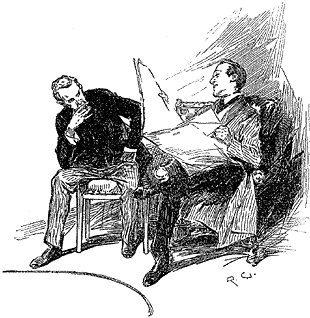
\includegraphics[%
  width=1.0\columnwidth]{images/study10-stud-24.png}\end{center}

\noindent \begin{center}\noun{{}``Didn't I tell you so when we
started?'' cried Sherlock Holmes with a laugh.}\end{center}
\end{figure}
{}``Didn't I tell you so when we started?'' cried Sherlock Holmes
with a laugh. {}``That's the result of all our Study in Scarlet:
to get them a testimonial!''

{}``Never mind,'' I answered, {}``I have all the facts in my journal,
and the public shall know them. In the meantime you must make yourself
contented by the consciousness of success, like the Roman miser\mdsh{---}

\begin{center} \footnotesize

\textit{```Populus me sibilat, at mihi plaudo} \\*

\textit{Ipse domi simul ac nummos contemplar in arca.'''}

\end{center}
\end{document}
